\documentclass[12pt,
bibtotoc,liststotoc,appendixprefix,
twoside=off,paper=a4,headings=small]{scrbook}
%
% Packages
% -----------------------------------
\usepackage[
  paper=a4paper,
  left=12.5mm,
  right=25mm,
  top=25mm,
  bottom=50mm,
  bindingoffset=10mm]{geometry}		% Seitenränder und Bindungskorrektur einstellen

\usepackage{amsmath,amssymb,amsfonts}
\usepackage{algorithmic}            
\usepackage{apacite} 				% Literatur-Referenzen: American Psycholog. Assoc.
\usepackage{natbib}	
\usepackage[style=iso]{datetime2}
\setcitestyle{round,aysep={}} 		% Indizierg. in runden Klammern, zw. Autor u. Jahr
%\usepackage[latin1]{inputenc} 		% Umlaute im Text
\usepackage[english]{babel}			% Rechtschreibg.
\usepackage[T1]{fontenc}
\usepackage{lmodern}				% Schriftfamilie
\usepackage{microtype}				% für die Mikrotypografie (besseres Schriftbild)
\usepackage{comment}
\usepackage{graphicx} 				% Grafiken einfügen (pdf,png - aber jpg vermeiden)
\graphicspath{{./Pictures/}}          % Pfad zu den Pictures

\usepackage{url}					% URL's formatieren (z.B. in Literatur) 
\usepackage{setspace} 				% Zeileneinstellung

\PassOptionsToPackage{hyphens}{url}
\usepackage[colorlinks,linkcolor=black,citecolor=black,urlcolor=blue]{hyperref} 				% für Hyperlinks in PDF-Dokumenten   

\usepackage{tabularx} 				% bessere Gestaltung von Tabellen
\usepackage{longtable} 		
\usepackage{multicol}				
\usepackage{multirow}
\usepackage{booktabs}
\usepackage{tabularx}
\setkomafont{disposition}{\bfseries}
\usepackage[active]{srcltx}
\usepackage{listings}				% Algorithmen

\usepackage{mdwlist}				% Listen

\newtheorem{mydef}{Merksatz}  		% Falls Beispiele, Merksätze m. fortl. Nr. gebr. werden
\newtheorem{bsp}{Beispiel}

%\usepackage{todonotes}				% zum Erstellen von ToDos im Editor

\usepackage{lscape}					% zum Rotieren von Seiten

\usepackage{amsmath,amssymb,amsfonts}				% zum Schreiben von mathematischen Formeln

\usepackage{xcolor}

\usepackage{parskip}

\usepackage[nopostdot,toc,acronym,nomain,nonumberlist]{glossaries}
\makeglossaries
\setacronymstyle{long-short}
\loadglsentries[acronym]{./Chapters/0_acro_list}
    
\usepackage{calc}

\usepackage{footnote}				% Fußnoten
\usepackage{tablefootnote}			% Fußnoten in Tabellen

%\clubpenalty = 10000
%\widowpenalty = 10000 \displaywidowpenalty = 10000

\hyphenation{voll-st\"andigen}		% Worttrennungen global definieren

\setcounter{tocdepth}{1}			% Ebenen, die im Inhaltsverzeichnis angezeigt werden
\usepackage{float}
% Document
% -----------------------------------
\begin{document}
\frontmatter 
    % Titelseite soll keine Kopf oder Fußzeile haben
\thispagestyle{empty}

% Alle Elemente sollen zentriert sein
\begin{center}

\vspace*{-10mm}

{\LARGE DEPARTMENT OF \\INFORMATION SYSTEMS\\[1mm]}
FREIE UNIVERSIT\"AT BERLIN\\

\vspace*{1cm}


\includegraphics[width=0.18\textwidth]{fu_logo}

\vspace*{1cm}

% Art der Arbeit
{\Large \textbf{Master Thesis}}\\ 
\vspace{1cm}
{\Large \textbf{Zero-Knowledge Proof Algorithms: A Systematic Literature Review and Application in the Aviation Industry}}\\ 


\begin{comment}
% Titel der Arbeit 
{\Large \textbf{Hier folgt der Titel}}\\ 
\vspace*{1mm}
{\Large \textbf{dieser kann auf bis zu drei}}\\ 
\vspace*{1mm}
{\Large \textbf{Zeilen verteilt werden wenn n\"otig}}\\
\end{comment}
\vspace{1.5cm}

% Name der Autorin
{\LARGE Elina Beletski}\\[15mm]

% Gutachter, Kontaktdaten und Abgabetermin
\parbox{120mm}
{
\begin{large}
\begin{tabbing}
Supervisor: \hspace{.7cm} \=Univ.-Prof. Dr. rer. pol. Natalia Kliewer\\[4mm]
Semester:\> Winter term 2022/23\\
Author:\> Elina Beletski\\ % alphabetische Reihenfolge (Nachname)
Student ID:\> 5504054\\
Address:\> N\"urnberger Str. 18, 10789 Berlin\\
Email:\> elina.beletski@fu-berlin.de\\
Phone:\>+4917620310530\\
Studies:\>M.Sc. Information Systems\\[8mm]
\textbf{Date:} \> \textbf{12 June 2023}\\
\end{tabbing}
\end{large}
}
\end{center}
\clearpage{\pagestyle{empty}\cleardoublepage}
 			% Titelblatt
    \newpage
    \clearpage{\pagestyle{empty}\cleardoublepage}
    \thispagestyle{empty}


\vspace*{1cm}

\begin{center}
    \textbf{Abstract}
\end{center}

\vspace*{1cm}

\noindent 
The following blindtext illustrates the length of the Abstract in english. Lorem ipsum dolor sit amet, consectetuer adipiscing elit. Aenean commodo ligula eget dolor. Aenean massa. Cum sociis natoque penatibus et magnis dis parturient montes, nascetur ridiculus mus. Donec quam felis, ultricies nec, pellentesque eu, pretium quis, sem. Nulla consequat massa quis enim. Donec pede justo, fringilla vel, aliquet nec, vulputate eget, arcu. In enim justo, rhoncus ut, imperdiet a, venenatis vitae, justo. Nullam dictum felis eu pede mollis pretium. Integer tincidunt. Cras dapibus. Vivamus elementum semper nisi. Aenean vulputate eleifend tellus. Aenean leo ligula, porttitor eu, consequat vitae, eleifend ac, enim. Aliquam lorem ante, dapibus in, viverra quis, feugiat a, tellus. Phasellus viverra nulla ut metus varius laoreet. Quisque rutrum. Aenean imperdiet. Etiam ultricies nisi vel augue. Curabitur ullamcorper ultricies nisi. Nam eget dui. Etiam rhoncus. Maecenas tempus, tellus eget condimentum rhoncus, sem quam semper libero, sit amet adipiscing sem neque sed ipsum. Nam quam nunc, blandit vel, luctus pulvinar, hendrerit id, lorem. Maecenas nec odio et ante tincidunt tempus. Donec vitae sapien ut libero venenatis faucibus. Nullam quis ante. Etiam sit amet orci eget eros faucibus tincidunt. Duis leo. Sed fringilla mauris sit amet nibh. Donec sodales sagittis magna. Sed consequat, leo eget bibendum sodales, augue velit cursus nunc, quis gravida magna mi a libero. Fusce vulputate eleifend sapien. Vestibulum purus quam, scelerisque ut, mollis sed, nonummy id, metus. Nullam accumsan lorem in dui. Cras ultricies mi eu turpis hendrerit fringilla. Vestibulum ante ipsum primis in faucibus orci luctus et ultrices posuere cubilia Curae; In ac dui quis mi consectetuer lacinia. Nam pretium turpis et arcu. Duis arcu tortor, suscipit eget, imperdiet nec, imperdiet iaculis, ipsum.

\begin{comment}
    1: -transparency and varifiability by design to solve challenges:
            - need for visibility and traceability of validation process for MRO spare parts and certificates in a trustless environment with high data confidentiality requirement (competitive information, personal information) -->zkDApp
    2: - fraud-preventive verification mechanisms by design to solve challenges:
            - lack of data structure because of paper-based documentation and no possibility to verify authenticity of MRO spare part documents 
    3: - expertise knowledge of zkps more closely related to aviation industry by systematic literature review and exemplary presentation of zk-SNARKs protocol steps 
\end{comment}
    \newpage
    \clearpage{\pagestyle{empty}\cleardoublepage}
    \onehalfspacing                  	% Zeilenabstand ab hier 1.5 zeilig
    \tableofcontents 					% Inhaltsverzeichnis
    \clearpage{\pagestyle{empty}\cleardoublepage} 
    
    \listoffigures 					 	% Abbildungsverzeichnis
    \clearpage{\pagestyle{empty}\cleardoublepage}
    
    \listoftables						% Tabellenverzeichnis rein
    \clearpage{\pagestyle{empty}\cleardoublepage}

    \printglossary[title={List of Abbreviations},type=acronym,style=long]
    \clearpage{\pagestyle{empty}\cleardoublepage}

% -----------------------------------
\mainmatter 							% die einzelnen Chapters
    \chapter{Introduction}
A modern civil aircraft consists of approximately three million parts, of which thousands of components must be maintained, repaired, and overhauled (MRO) throughout its life cycle. These MRO events have to be documented. If aircraft and accompanying components demonstrate safe technical conditions, aviation authorities declare them airworthy and allow them to operate. Considering there are 25,000 commercial aircraft in operation and approximately 20,000 suppliers in the industry, hundreds of millions of events must be documented and verified \citep{mroBCservices1}.
\section{Motivation}
The aviation industry is characterized by high competition and mistrust among the stakeholders \citep{Chatzi2019TDoC}, creating conflicting expectations when digitalizing and automating its processes. The aircraft part lifecycle starts with initial manufacturing documentation and continues with buying, selling, leasing, repair, overhaul, and disposal documentation. To this day, back-to-birth documentation of aircraft and components is still largely paper-based and lacks digital process automation \citep{efthymiou}. Transparency and traceability are compromised through disconnected, scattered MRO event documentation entries across various enterprise resource planning systems operated by the industry's participants \citep{mroBCservices1}. Aircraft components without verified back-to-birth documentation history have no value, i.e., more sustainable secondary parts trading is impossible. This overall situation has an immediate effect on the verification of aircraft parts documentation by aviation authorities: verifying for airworthiness and traceability in the event of an accident is a cumbersome, inquiry-based process, which leaves room for withholding of information and counterfeit parts \citep{planecrash}. 
The research project RAPADO drives digitalization in the aviation industry by creating an industry standard for seamless documentation and verification of aircraft spare parts. One of the research goals is to accumulate knowledge about blockchain technology and investigate its applicability to the MRO industry. Research is conducted by the Information Systems Department at Freie Universit{\"a}t Berlin in collaboration with project partner Opremic Solutions GmbH.

Current work on blockchain in the MRO industry focuses on empirical analyses of the benefits of the technology in general and the willingness to adopt \citep{efthymiou}. At the same time, further technical understanding and prototypical implementations must be performed. Project-related work resulted in further research into the application of blockchain technology to target the requirements of document storage and traceability, excluding the scope of state-of-the-art cryptography. Previously, a blockchain-based file storage system was proposed, prototypically developed as a decentralized application (DApp), storing aircraft part certificates in a distributed file storage system. Certificate data is traceable through a file hash, which is persisted on-chain. This preliminary work concludes with zero-knowledge proofs as the next step in project-related research \citep{ZedelJ}. Aircraft parts documentation history should always be verifiable and tamper-proof while preserving data confidentiality and protecting the identity and ownership of industry participants \citep{Wickboldt2019BlockchainFW}. The aspect of decentralized verification with the requirement of data privacy preservation still needs to be addressed.

Zero-knowledge proofs can facilitate such a verification process without revealing sensitive information. Due to the possibility of combining confidentiality and transparency, and scaling blockchain throughput, interest in zero-knowledge proofs increased. However, their potential application in the aviation industry needs further assessment. This master thesis focuses on verification and information confidentiality requirements for aircraft spare parts documentation. Suitable use cases and their implementation through zero-knowledge proofs are investigated. The research question is formulated as follows:

\begin{center}
\textit{How can zero-knowledge proofs be utilized to satisfy requirements and implement identified use cases for the aircraft spare parts documentation?}  
\end{center}

\section{Contribution Outline}
In this sub-chapter, the following aspects of contribution are outlined. The topic of zero-knowledge proofs is complex and needs to be discussed separately, as concluded in preliminary research. A systematic literature review, based on the methodology in \citet{vomBrockeJan2019TDgs} and \citet{Webster2002AnalyzingTP}, surveys current research results and accumulates expertise in the field. As a more practical result, a ZKP protocol, i.e., Groth16, is applied step by step to provide an overview based on a simple polynomial example. Specific details for understanding the protocol support the mathematical example, forming a reference document acting as the first artifact of the thesis.

Current research requirements in the project RAPADO are revisited to derive implementation requirements and select use cases. Taking up the use case of MRO data attestation and verification, the developed zero-knowledge decentralized application (zk-DApp) is a proposal to balance transparency and data confidentiality. The zk-DApp is evaluated based on performance aspects and feedback within the project.

For all existing software implementations within the project, high-level assumptions about a digital data structure for aircraft spare part documentation were necessary to continue with prototype development. The question of a practical, blockchain-compatible data structure was not yet addressed and reoccurred as a feedback point during discussions in the project. Motivated by the use case of authenticity checks of spare part certificates and as an evaluation result of the zk-DApp mentioned above, a ZKP and Merkle-tree-based data structure based on \citet{sedlemeirgrenenergy} is introduced. Concluding with the data structure proposal, a direction of future research is suggested, considering existing software artifacts and results.

\section{Structure}
This master thesis is structured as follows. Chapter 2 summarizes related work, separated into project-related work, zero-knowledge proof topic-related work, and related systems. Chapter 3 describes the execution of the systematic literature review methodology, the artifacts' implementation approach, and summarizes key findings. Chapter 4 presents the outcomes of the systematic literature review, structured from the perspective of historical and design-oriented classification of zero-knowledge proofs. Chapter 5 summarizes implementations and results. First, the requirements are summarized. Second, the three artifacts are described, each satisfying a requirement. The first artifact is the example calculation and step-wise computation of the Groth16 algorithm. The second artifact is the zk-DApp for MRO data attestation and verification. Subsequently, the zk-DApp is evaluated, resulting in the third artifact's design. The third artifact is the fraud-preventive zero-knowledge data structure for data authenticity and integrity verification. Chapter 6 concludes this master thesis by summarizing key findings, describing identified limitations, and providing a future outlook for research.


    \clearpage{\pagestyle{empty}\cleardoublepage}		% löscht Kopfzeilen und Seitennummerierung von der letzten Seite eines Chapters, sofern dort kein Text mehr steht
    \chapter{Related Work}
Zero-knowledge argument systems are algorithms resulting from specific designs of proof systems combined with cryptographic primitives and mathematical tools. This chapter summarizes content-related and project-related work, as well as related systems associated with this master's thesis. Related to the project RAPADO, current and previous research and implementation efforts at the department of information systems at Freie Universit{\"a}t Berlin are described. Related to the selective systematic literature review in chapter 5, main knowledge surveys are presented to be referred to for further information. The results of this master's thesis are a step-by-step example computation of the Groth16 protocol, a zero-knowledge DApp software artifact and a verification mechanism architecture conceptual artifact. The related systems utilized for artifact development are presented in this chapter.

\subsubsection{Project-related work}
Preliminary research at the Department of Information Systems focuses on the architecture of suitable blockchain-based platforms for aviation industry MRO documentation. \citet{WickboldtMeiseKliewer} proposes a framework to use a private blockchain-based architecture in HyperLedger Fabric, whereby node registration is managed through trusted Membership Service Providers (MSP). This first approach resulted from initial core requirements of data persistence, selective data access, data integrity, and transparency of back-to-birth documentation histories \citep{WickboldtClemens2018BzdD}. Subsequently, these core requirements were further specified through extensive information exchange with previously identified stakeholder groups of airline companies, MRO full-service providers, and MRO parts merchants \citep{ZedelJ}. Further research proposed a public blockchain-based platform with smart contracts and a decentralized file storage system \citep{ZedelJ}. MRO documentation is stored in the decentralized file storage system, which produces a unique file hash. It also identifies the document that is implemented as a non-fungible token (NFT) in a smart contract. Following the identified process, the validation status set by aviation authorities is captured. In a DApp software artifact, aviation authorities get full document access using threshold encryption. They receive their key shares from the smart contract and can decrypt them using their private key. By combining their key shares, the corresponding document can be decrypted, accessed, and used for verification. Hence, access management is not central because various nodes in the network have to combine their key shares. However, once access is granted, all data is exposed. Documents contain competitive information and must be treated confidentially. This led to further research on how to verify MRO documentation without fully exposing sensitive information. Zero-knowledge proofs were identified as promising technology to meet the requirement of data confidentiality during the verification of MRO documents on a public blockchain-based platform \citep{ZedelJ}. This master's thesis extends previous research by focusing on the topic of zero-knowledge proofs and applications for sensitive data verification.

\subsubsection{Content-related work}
In \citet{Thaler}, a in-depth survey is provided on the history of verifying computation and content classification of probabilistic proofs. Furthermore, more practical argument systems are described and their composition is studied, while provisioning the reader with a bird's eye view on the proof systems and cryptographic primitives needed to understand those. First, interactive, multi prover interactive, interactive oracle, probabilistically checkable proof systems and variants are described in more detail, introducing concrete examples proof systems from historical breakthrough in the beginning of research towards zero-knowledge argument systems. Second, relevant cryptographic primitives and mathematical tools are introduced, that enable non-interactivity, efficiency and zero-knowledge. Lastly, the reader is presented with a taxonomy of succinct non-interactive arguments of knowledge (SNARKs).

The current and compact work of \citet{chen2022review} surveys zk-SNARKs from a technical perspective. First, the historical development of zk-SNARKs is described. Second, the first state-of-the-art zk-SNARKs, the Pinocchio protocol is analyzed in great detail, and compared to its successor Groth16. Third, two main use cases of zk-SNARKs are highlighted, financial and rollup applications. Lastly, novel circuits are introduced, applied in the domain of private auctions and decentralized card games, and the implementation code is provisioned. A future research outlook is portrayed by introducing the current research status on zk-STARKs and recursive SNARKs.

A shorter survey on verifiable computation is provided by \citet{Ahmad}, whereby the chronological summary of theoretical and practical advances are at focus. Approaches are summarized according to their functionalities and analyzed according to their contributions. The authors provide comments on open challenges in verifying computation and give a future outlook for research efforts. 

Zk-SNARKs are the main focus in \citet{NitulescuGentleIntroSNARKs}. First, properties are defined and tools for designing zk-SNARKs are described. Second, SNARKs from probabilistically checkable proofs, quadratic arithmetic programs, linear interactive and polynomial interactive oracle proof systems and variants are introduced, whereby more practical use cases are highlighted. 

\subsubsection{Related systems}
Based on the smart contract for zkDocs created by \citep{zkdocs}, the zk-DApp for MRO data input verification is implemented and described. For this use case, additional operators and a new schema are added and changes to the frontend implemented. The description of the implementation is in 6.2. In contrast, the non-zero-knowledge DApp implementation developed during the RAPADO semester project uses encrypted and decrypted key shares via the secrets.js library, which are combined to view and validate a MRO certificate for a specific part. For the previously developed DApp, the focus is to create a first structure to upload MRO certificates. The validation implementation using only Shamir's secret sharing is vulnerable. The zk-DApp implementation focuses on the equilibrium of privacy and transparency requirements for performing attestation and verification of specific MRO data and digitization concepts. It is achieved through a thorough examination of the technicalities of zero-knowledge proofs and their application as per current research. The data points chosen for the prototype resulted from previous, not yet seized requirement analyses in the project and can be exchanged at any time in the future. 

The second prototypical artifact is a architecture proposal for MRO data digitization with the aim to preserve data confidentiality while offering requirement-sufficient transparency via zero-knowledge proofs and merkle trees. A similar first attempt is presented in SOURCE for trading green energy certificates. 
%on chain computations are expensive (see project semester), ZKPs are powerful off chain solutions for verification processes
%zkDocs smart contract and framework used for MVP
%- Sedlmeier, V{/"u}lter, Str{/"u}ker (2021): trading green energy certificates: same problem of verification vs privacy, Implementation architecture based on zk RollUps, very good reasoning about requirements (same as Rapado), maybe a good starting point to create an architecture as second artifact for rapado? architecture to verify information about certificates
    \clearpage{\pagestyle{empty}\cleardoublepage}
    \chapter{Methodology}
The research concept of the thesis is divided as follows: first, a systematic literature review (SLR) will be conducted according to \cite{HevnerAR2004DSiI, vomBrockeJan2019TDgs, Webster2002AnalyzingTP}. Second, Knowledge from the first part will be applied to the project RAPADO. The implementation part of this master's thesis follows an agile development approach. RAPADO use cases for zero-knowledge proof protocols are investigated, conceptualized, and evaluated, considering aspects found in previously examined literature and preliminary work at the department of information systems at Freie Universit{\"a}t Berlin. The application of acquired technical and theoretical knowledge is at focus, while the use cases implemented can be exchanged in the future during further project research. 

\section{Systematic Literature Review}
The initial and current status and results of project RAPADO are reflected on. From this analysis, potential use cases and design requirements for the application of zero-knowledge proofs are derived. Following the requirement to accumulate knowledge within the project in order to build expertise in blockchain-based development for the aviation industry, the literature survey focuses on the design of zero-knowledge proofs and theoretical foundations. Opportunities and challenges are displayed by considering practical examples. The second part of the research concept is the implementation of a zero-knowledge application for the use case of MRO data attestation and verification, whereby the demonstration of technical mechanisms is at focus.

This master's thesis is associated with preliminary work carried out within RAPADO at the department of information systems. Immediate previous research concludes with conceptual solutions and a decentralized application for aviation industry MRO documentation, centering storage and traceability \citep{ZedelJ}. Hereby, use cases of uploading, storing, and trading aircraft spare parts certificates were given and specific blockchain platform architectures were used. This research extends previous findings. However, it takes a new perspective by further investigating possible use cases for ZKP as methods of automating verification processes, preserving data confidentiality and suggesting suitable data formats. The results are expected to represent the broader research project, i.e., beyond previously used software.

The focus of the SLR are zero-knowledge proofs with the scope of classification, opportunities, challenges, evaluation methods, and examples in practice. The design of zero-knowledge proofs needs to be understood from a theoretical perspective. Application domains and use cases applicable to the research project are at focus, which excludes topics of cryptocurrencies and embedded systems. The objective of this survey is to provide an extensive overview on the design and implementation of zero knowledge proofs, as well as to bring out practical and critical implications within the domain of distributed ledger technology. The final search string is derived from a concept map (Figure \ref{fig:concept_map}) and the literature found is summarized through a concept matrix(FIGURE). 

\begin{figure}[hbt]
	\centering
		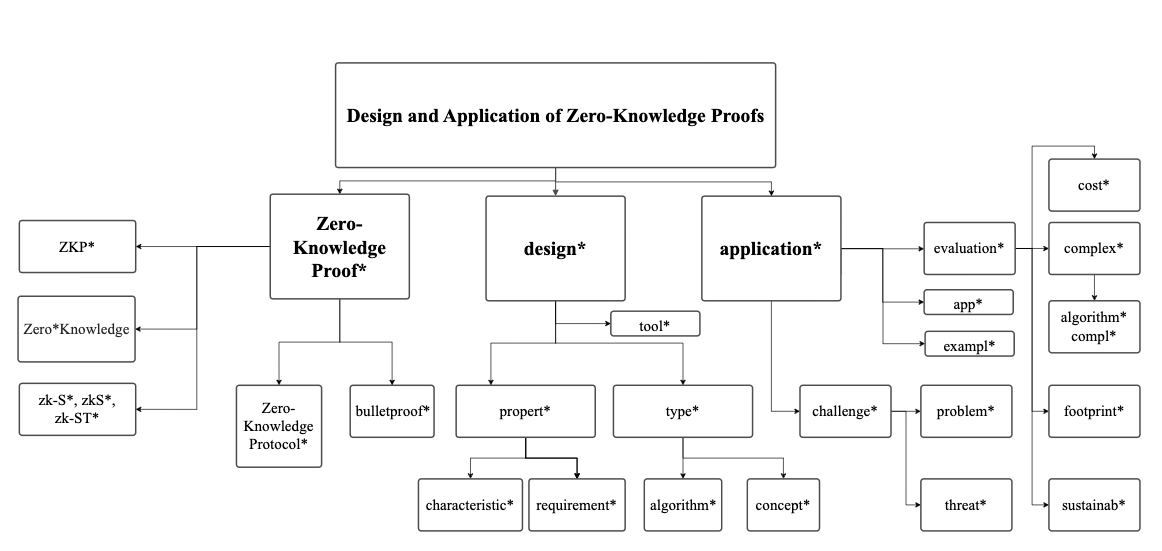
\includegraphics[width=0.99\textwidth]{Pictures/concept map.png}
	\caption{Search compression process}
	\label{fig:concept_map}
\end{figure}

The research question is assigned to topics of Computer Science, Mathematics, and Information Systems. For the search, the databases Web of Science (WoS), Association of Computing Machinery (ACM), zbMATH, arXiV, Association of Information Systems (AIS), and Institute of Electrical and Electronics Engineers (IEEE) were queried. Articles were searched in Title, Keywords, and Abstract, and if possible, with date restrictions back to 2018 (WoS) and 2006 (ACM). The following search string was used: (("ZKP*" OR "Zero-Knowledge*" OR "zero*knowledge*algorithm*" OR "zero*knowledge*protocol*" OR "zero*knowledge*proof*" OR "zkS*" OR "zk*SNA*" OR "zk*STA*" OR "zk*STO" OR "bulletproof*") AND ("application*" OR "example*" OR "app*") AND ("carbon*footprint*" OR "*complexity*" OR "evaluation*" OR "cost*" OR "sustainab*" OR "environment*") AND ("challenge*" OR "threat*" OR "problem*"). After deduplication, the search resulted in 580 hits, which were condensed according to the following approach. First, the result was filtered by English or German resources which have more than or equal to five citations with three times or higher past 180 days usage (560 hits). The next exclusion criteria were applied in Title and Keywords (396 hits), Abstract (319 hits), and Full-text (80 hits), of which backward/forward search added another 20 hits. 

\begin{figure}[hbt]
	\centering
		
\includegraphics[width=0.99\textwidth]{Pictures/bsp1.png}
	\caption{Concept Matrix}
	\label{fig:concept_matrix}
\end{figure}

Results of the survey can be summarized into the following topics. 
\begin{itemize}
    \item Algorithm design topics: Zero-knowledge proofs are designed by combining proof systems and cryptographic means to achieve specific characteristics. Proof systems are examined and defined, linking and presenting cryptographic tools within the scope of building zero-knowledge argument systems in the area of applicable blockchain-based solutions.
    \item Subsequent to the previous item, most widely used and performative zero-knowledge proofs are described in more detail, i.e., algorithms of specific zk-SNARKs, zk-STARKS, and Bulletproofs.
    \item Selective literature is summarized according to the following problem domains identified: Electronic Voting and Government, Electronic Auctions, Data Queries and Traceability, Electronic Healthcare, Cloud Security, and Scaling.
    \item Opportunities and challenges are summarized and aligned by evaluating and comparing the different algorithms qualitatively through literature review and quantitatively through complexity analysis.
\end{itemize}

\section{Implementation and Evaluation}
Results of this masters' thesis are three artifacts, each satisfying a requirement in project Rapado. The requirements are derived from previous work at the department of Information Systems at Freie Universit{\"a}t Berlin and workshops held within the project consortium. From these broader requirements, specific design requirements are extracted, which can be referred to during implementation. The development of artifacts is conducted in an agile and iterative manner, whereby the demonstration of the technical application of zero-knowledge proofs is at focus. The following table describes the three artifacts and their implementation approach (Table \ref{tab:summary_artifacts}). The project and design requirements are further described in the fourth and sixth chapter. 

The algorithms studied in chapter 5 are evaluated according to their complexity. Artifact 1 represents a reference document to understand zk-SNARKs functionalities. It is shown in the final state after recurring consultation between author and research department. Artifact 2 results from an agile implementation approach and is evaluated through first feedback collection from the project partner. Enhancements are implemented and summarized in chapter 6. Artifact 3 is evaluated by revisiting project and design requirements to assess current and future project needs. 

\setlength{\tabcolsep}{2ex}
\renewcommand{\arraystretch}{1.5}%
\begin{table}[htb]
	\centering
	    \caption{Results and Implementation Description}
		\begin{tabular}{|m{0.001\linewidth} | m{0.12\linewidth} | m{0.35\linewidth} | m{0.4\linewidth} |}
		\hline
		\textbf{}& \textbf{Artifact} & \textbf{Short Description} & \textbf{Implementation} \\ \hline
            1&Groth16 Example \newline Calculation & Step-wise computation of Groth16 protocol by taking a simple polynomial as example. The goal is to create a reference document to underline zk-SNARKs functionality, corresponding to the requirement of accumulating expertise on the topic within the project. & Developed during research phase on zk-SNARKs theory and functionality by taking a simple proof example and following the Groth16 protocol steps \citep{Groth2016OnTS}. \\  \hline
            2&zk-DApp MRO \newline Attestation & Zero-knowledge decentralized application to attest to MRO data of parts and create a trusted verified process. & Agile development with focus of demonstrating the functionality of plonk zk-SNARKs and practical implementation with circom and snarkjs. First feedback is collected and implemented. \\ \hline 
            3&Zero-Knowledge Data \newline Structure & Motivated by recurring comments during workshops and project consortium meetings, this is a first architecture prototype to enable further discussion of effective data formats and digitization of spare parts and corresponding documents. & Analyzing similar efforts in other alternative fields of research \citep{sedlemeirgrenenergy}, key insights are combined with results from the literature survey to implement first ideas and approaches to utilize zero-knowledge proofs to create effective data formats and standards for the future of aviation. \\  \hline 
	\end{tabular}
\label{tab:summary_artifacts}
\end{table}
\begin{comment}
-review of project requirements-->ableiten von design requirements
- with focus at technical functionalities, two use cases were picked out and developed in an agile manner, presenting very first prototypes for open discussion further in the project, main goal of knowledge accumulation is satisfied in chapter 5, designed and implemented artifacts satisfy two other main project requirements
- evaluation according to complexity analysis, fit to the project needs, limitations and future outlook
\end{comment}




\begin{comment}
SLR
Analysis of other resources
--> ends with requirements
(how good/bad the solution is)
-quantitative and qualitative evaluation, e.g. Laufzeit und Interviews 
- say what is not in scope
-DO NOT describe some agile method for the sake of having it! Just say it is a rather agile method etc.

I. Systematic literature review according to vom Brocke, Cooper and Webster: 
    1. Definition of Scope
        - classification, examples, challenges and evaluation methods of zero knowledge proof protocols 
        
    2. Conceptualization
        - work with concept map
        - derive at a search string
        
    3. Literature Search and Selection
        - look for review paper first to get good overview about the topic
        a) exclude paper that are too old and have too few citations and/or low impact factor (e.g. 5.5 is high)
        b) exclusion acc. to title and keywords
        c) exclusion acc. to abstract & structure of paper & RQ
        c) exclusion acc. to full text & availability of resource
        
    4. Synthesizing of Literature
        - cluster definitions, examples, drawbacks and evaluation methods (first suggestion can be found in the preliminary agenda)
        - write overview section about ZKP (Chapter 4)
- - - - - - -
How to know if a paper is useful for me?
1.title 2.keywords 3.abstract 4.structure of the paper 5.examples/use cases 6.research question/formal problem definition
- - - - - - -
% DSR muss nicht sein, kann auch SCRUM oder {"a}hnliches
II. Design Science Research
- DSR method acc. to Peffers and Hevner

\end{comment}
\begin{comment}
2) Ziel der Arbeit, scope of work
- not scope to practically integrate any of the concepts into existing DApp or any other existing system
- welche use cases gibt es f{"u}r ZKPs in RAPADO
- wie k{"o}nnte man diese Umsetzen

4) Ergebnisse skizzieren
- implementation can be a proof of concept, software artifact depends highly on complexity of the use case
\end{comment}
    \clearpage{\pagestyle{empty}\cleardoublepage}
    \chapter{Zero-Knowledge Proofs}
This chapter surveys selective literature about zero-knowledge proofs for practical design applications. The goal is to familiarize the reader with the content classification of zero-knowledge proofs in cryptography and to give an introduction and comparison of the central argument systems widely used today. 

Zero-knowledge proof systems belong to the domain of verifiable computation \citep{Simunic, Ahmad}. Verifiable computation (VC) uses cryptographic protocols and arguments to verify that a computation was performed correctly. The introduction of interactive proof systems (\acrshort{ip}s) by \citet{GoldwasserIPs} and \citet{BabaiIPs} shows that only correct proofs are valid and malicious proving strategies cannot be verified. Traditional proofs are static and are made for easy, step-wise computation verification, whereas \acrshort{ip}s require interaction between the prover and verifier. In computational complexity theory, interactive proof systems are abstract machines exchanging messages between the prover and verifier to convince the verifier that these strings belong to a language \(L\). Here, the formal language \(L\) defines a decision problem, but i.e., a computational problem with binary classification, yes and no. Examples of sets of strings in \(L\) can be that a specific Bitcoin transaction is valid, \(x = 7\) for a given \(f(x)\), or a particular object belonging to a specific Merkle tree. The untrusted prover has unlimited computational power, and the verifier is honest and computationally restricted. 

Advances in computational complexity theory during that time showed that \acrshort{ip}s are more efficient and belong to a broader class than the traditional NP, i.e., problems solvable in deterministic polynomial time by reading proof strings of polynomial length \citep{IOPsdisc}. In 1987, it has been shown that every language belonging to NP has zero-knowledge proof systems \citep{anymental10.1145/28395.28420}. Later, it has been proven that the class of \acrshort{ip}, i.e., problems solvable by interactive proof systems, lies in PSPACE, i.e., problems solvable in polynomial space \citep{Shamir10.1145/146585.146609} and that every language \(L\) in polynomial time has an interactive proof system \citep{Lund10.1145/146585.146605}. The complexity class of \acrshort{ip} describes prover and verifier interaction in a polynomial number of rounds. Other important advances in computational complexity theory are \acrshort{mip}=NEXP \citep{Laszlo} and the \acrshort{pcp} theorem \citep{PCPTheorem}. These works resulted in a set of proof and argument systems that will be introduced in this chapter. \citet{Thaler} gives an exhaustive overview of all systems and in-depth protocol descriptions. 

The following examined proof systems are secure against computationally unrestricted provers: Interactive Proofs (IPs), linear Probabilistically Checkable Proofs (\acrshort{pcp}s), and Interactive Oracle Proofs (\acrshort{iop}s). 

Combining the systems above with cryptographic tools to force specific behavior in the proof generation will create an argument system. Argument systems are considered zero-knowledge if the proof reveals nothing but its validity \citep{GoldwasserIPs}. Adding certain properties, e.g., non-interactivity, succinctness, and knowledge, will design a specific argument of knowledge, e.g., \acrshort{zksnark} (zero-knowledge succinct non-interactive argument of knowledge). Different \acrshort{zksnark}s and notions will be examined in more detail.

The following sub-chapters are structured according to the design-oriented approach described above:
\begin{itemize}
    \item IPs, and \acrshort{iop}s are defined. Through the combination of polynomial commitment schemes or cryptographic tools, argument systems can be designed. Non-interactivity is achieved through the Fiat-Shamir transformation.
    \item Properties and mathematical tools are introduced to describe different arguments of knowledge: \acrshort{zksnark}, \acrshort{fri}-STARK, and bulletproofs. Real-world applications of zero-knowledge proof systems are summarized.
    \item The different proof systems are evaluated according to computational complexity, communication, and security.
\end{itemize}

\section{From Proof Systems towards Argument Systems}

A mathematical proof in the context of computer science and cryptography is any object that convinces a verifier that a statement is correct. Mathematical proofs embody what is defined in the complexity class NP. A proof system is a structured scheme that decides whether a statement is correct or incorrect. Three properties are desirable for proof systems \citep{GoldwasserIPs}, which will be introduced shortly. Throughout this chapter, these properties are revisited more exhaustively.
\begin{itemize}
    \text{\parbox{420pt}{
    \item The procedure to create and verify proofs should be \textbf{efficient and fast}. 
    \item \textbf{Completeness}: True statements should have convincing proof of their validity.
    \item \textbf{Soundness}: If a statement is incorrect, there is no possibility of it having convincing proof.}}
\end{itemize}
Unlike argument systems, proof systems do not limit the malicious prover in its computational power (statistical soundness). Using cryptographic primitives and restricting the prover, e.g., probabilistic polynomial time proof, so that it cannot break the primitives, describes the design towards argument systems, which are computationally sound \citep{ArgSystems, MicaliArgSys}. Each proof system presented makes assumptions about the prover. However, only with cryptographic tools and zero knowledge can these proof systems be extended with additional properties to yield zero-knowledge argument systems of various kinds.

\subsection{Interactive Proofs}
In interactive proof systems, the prover with unlimited computational resources interacts with a computationally bound verifier to convince the verifier of the correctness of a statement. The verifier randomly challenges the prover, which is called coin tosses \citep{GoldwasserCoinTosses}. These challenges happen in rounds until sufficient tests are run, and the verifier is convinced. \citet{GoldwasserIPs} defined an interactive proof system that is private, i.e., that the verifier's challenges are not publicly accessible, whereas the interactive proof system of \citet{BabaiIPs} allows the coin tosses to be publicly accessible by the prover.
\begin{align*}
    \text{\parbox{450pt}{\textbf{Interactive Proof System.} \textit{\(L\) is a language over \(\{0,1\}^n\), with n representing the input size domain of n-bit strings. An interactive protocol is an interactive proof system if, after \(k\) rounds, the probabilistic verifier in polynomial time exchanged \(k\) messages with the computationally unrestricted prover and has to either accept or decline the correctness of the prover's proposition. IP is the complexity class of problems solvable by a k-round interactive proof system.}}}
\end{align*}
The transcript is the order in which messages are exchanged. The prover and verifier are functions \(P(x), V(x)\) with common input \(x\). The overall distribution of all transcriptions between the prover and verifier is called \(View_V(P(x), V(x))\), which is bound by the number of rounds between \(P\) and \(V\). \(P\) provides a result that satisfies the proposition, e.g., \(y\) to a function \(f(x) = y\). \(P\) and \(V\) exchange a transcript of messages \((m_1, m_2, m_3, ..., m_k)\), whereby both parties take turns, and the prover sends the last message. Note that \(V\) is probabilistic with internal randomness \(r\). Hence, the output depends on \((V, x, r, P)\) and is \(\{0,1\}\), i.e., \(1\) if the statement is correct, and \(0\) if it is incorrect \citep{GoldwasserIPs, BabaiIPs}. Interactive proof systems have completeness error \(\delta_c\) and soundness error \(\delta_s\) . For any input \(x\), there must be a convincing proof that \(f(x)\) is correct. Incorrect statements for \(y \neq f(x)\) cannot result in a convincing proof, i.e., a malicious prover does not exist. \acrshort{ip} systems are valid if \(\delta_c, \delta_s \leq 1/3\) \citep{Thaler}. \acrshort{ip}s with \(k\) provers are multi-prover interactive proofs (\acrshort{mip}s), introduced by \citet{MIPsBen} and extended by \citet{MIPsSetty} to allow for the design of succinct arguments. \acrshort{mip}s are characterized by no information sharing and non-adaptivity of provers. The probabilistic polynomial time verifier acts similarly as in \acrshort{ip}s, but the challenges sent are not shared among the different provers. The prover's response \(i\) does not depend on the \(i-1\) interactions in the transcript, i.e., the prover cannot react based on the previous messages, because there is at least another prover \(p_j\) whose messages are not known to \(p_i\) for \(i\neq j\).

\begin{comment}
Some definitions are still missing:
randomness
completeness
soundness
statistical soundness
computational soundness
\end{comment}

\subsubsection{Non-interactive, Publicly Verifiable Arguments}
The Fiat-Shamir transformation transforms any interactive proof system based on public coin tosses into a non-interactive, publicly verifiable system. This transformation can be described effectively with the use of an ideal cryptographic assumption, the random oracle model (\acrshort{rom}). 
\subsubsection{Random Oracle Model}
The\acrshort{rom}methodology was introduced in cryptographic theory to satisfy the goal of designing secure cryptographic protocols. First, an ideal system is designed to give all parties access to an oracle, i.e., a random public function. Once the security of the protocol is proven, the random oracle function is replaced by a cryptographic hashing function to implement the system in practice \citep{ROMBellare}. In \acrshort{ip}s, the random oracle function is part of the view, i.e., random choices of challenges simulator output. It is assumed that the prover and verifier can query the random oracle function \(f_R\) by sending an input \(x\) so that the random oracle returns \(f_R(x)\). In \acrshort{rom}, the efficiency is dependent on x, i.e., for every input in the problem size domain \(D\), \(f_R(x)\) is captured. Since it is only practical in theory, because \(|D|\) is large to ensure security, e.g., \(2^{256}\), hash functions are used in practice \citep{ROMBellare, Thaler}, e.g., POSEIDON or SHA-3. The \acrshort{rom} is controversially discussed in retrospect: On the one hand, it is argued that there exist protocols that are only secure in the \acrshort{rom}, and all implementation efforts in practice have led to insecure protocols, whereby the security of the ideal scheme is not maintained. The area of work at focus is digital signatures and public-key encryption, showing that the \acrshort{rom} is not sound \citep{ROMCanetti}. On the other hand, this conclusion is discussed to indicate there is no evidence of practical security weaknesses if there is a need for random oracle systems in a protocol. Protocol design examples support this statement, e.g., Elliptic Curve Digital Signature Algorithm (ECDSA), leading to cryptographic insecurity if not using a random oracle \citep{ROMretroKoblitz}. 
\subsubsection{Fiat-Shamir Transformation}
The Fiat-Shamir transformation (\acrshort{fst}) \citep{ROMFiat1986HowTP} removes the need for prover-verifier interaction in a public coin interactive proof system with the help of the random oracle function. The result is a non-interactive, publicly verifiable system. \acrshort{ip}s send messages between the prover and verifier, whereby the verifier challenges the prover randomly. Every message the verifier sends in the \acrshort{ip} is replaced by values obtained by querying the random oracle. The query always depends on the previous message sent by the prover to prevent soundness attacks.

In summary, the prover only sends one message containing the transcript, i.e., the list of all messages sent by the prover and the query results of the random oracle. The input x has to be appended to the list every round. The verifier's coin tosses are no longer needed, and the verifier does not need to send messages to the prover (Figure \ref{fig:FST}).
\begin{figure}[hbt]
	\centering
		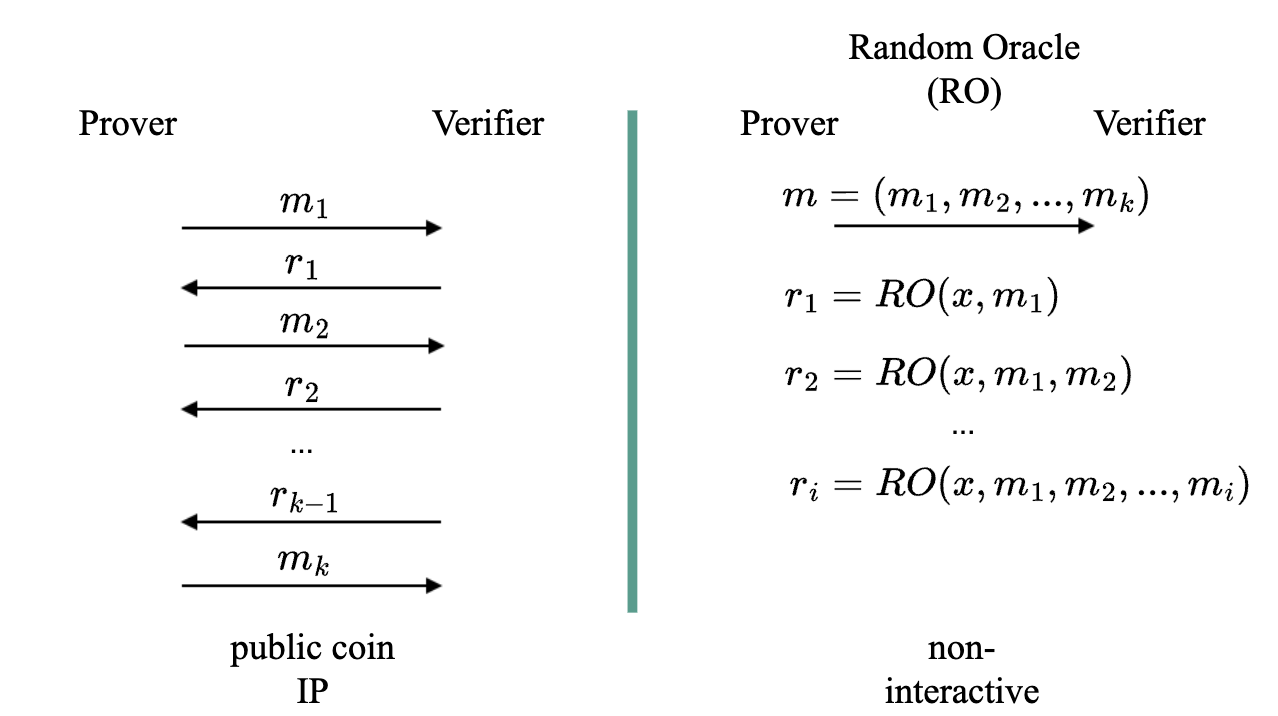
\includegraphics[width=0.8\textwidth]{Pictures/FST.png}
	\caption{Illustration of Generic Fiat Shamir Transformation (based on \citet{Thaler})}
	\label{fig:FST}
\end{figure}
Argument systems are obtained by applying polynomial commitment schemes to proof systems, while the prover commits to a low-degree polynomial. It allows for polynomial evaluation verification without possessing all the information of this polynomial. Polynomial commitment schemes are used to prove that a polynomial, evaluated at a specific input, results in a specific output. The prover commits to the polynomial, acting as some object hiding the polynomial, e.g., similar to a hash. The verifier challenges the commitment with a random value. The committer then creates a proof that the polynomial evaluates at that random value at a specific point. The polynomial itself is not revealed. In interactive proof systems with an honest prover running in polynomial time, any arithmetic circuit can be evaluated \citep{GKR10.1145/1374376.1374396}. Arithmetic circuits have gates that operate on two types, i.e., addition and multiplication. Besides gates, some wires carry integer variables. Retrospectively, it is a significant achievement since arbitrary computer programs can be expressed via arithmetic circuits, the base layer of many zero-knowledge protocols today. More mathematical tools for understanding the functionality of argument systems are covered in Chapter 4.2.
\subsubsection{Zero-Knowledge}
If the verifier knows nothing about the statement and the witness but its validity, the algorithm will run with zero knowledge. This property can be described by using a simulator notion \citep{Thaler}: A prover and probabilistic polynomial time verifier strategy exists under the honest verifier assumption. For any probabilistic polynomial time verifier strategy, there is a probabilistic polynomial time algorithm (simulator) that can depend on the verifier strategy, which produces outputs that are indistinguishable from the distribution of transcripts generated through the prover and verifier strategy interactions. The simulator ensures that the verifier only learns that \(x \in L\). Under the honest verifier assumption, there are at least six types of zero-knowledge protocols, whereby the notion of simulator output and transcript distribution being indistinguishable is at focus \citep{zktypes}:
\begin{itemize}
    \item \textbf{Perfect Zero-Knowledge}: The output of the simulator \(S(x)\) and the distribution of the transcript created through prover and verifier strategy interaction \(View_V(P(x), V(x))\) within the protocol is identical. 
    \item \textbf{Statistical Zero-Knowledge}: \(S(x) \text{ and } View_V(P(x), V(x))\) have a negligible statistical distance, given a polynomial number of samples from the distributions.
    \item \textbf{Computational Zero-Knowledge}: \(S(x) \text{ and } View_V(P(x), V(x))\) can be distinguished with negligible probability only if a polynomial number of samples is given.
\end{itemize}
Soundness is divided into statistical (for proof systems) and computational (for argument systems) soundness. Argument systems are computationally sound, i.e., allow for applying cryptographic primitives. The computationally bound prover cannot break these primitives, unlike the unbound prover in proof systems, which are statistically sound \citep{Thaler}. The verifier learns that a statement is true and has to be convinced that the prover knows a correct witness. The simulator is able to extract that witness information through interaction with the algorithm (knowledge soundness) \citep{NitulescuGentleIntroSNARKs}.

\subsection{Linear Probabilistically Checkable Proofs}
Probabilistically checkable proofs (\acrshort{pcp}s) differ from previously introduced proofs because the prover does not need to answer queries based on the current or previous query content posted by the verifier. The polynomial time verifier is provided with oracle access to a static proof string \begin{math} \pi \end{math}, whereby the proof is queried, and the result of it only depends on the currently processed query \citep{PCP}. The breakthrough of robust, pairing-based schemes is attributable to \citet{GennaroLinPCP}, who introduced Quadratic Arithmetic Programs (\acrshort{qap}s) as a variant of quadratic span programs. Quadratic span programs are efficient because they only satisfy boolean circuits. Therefore, introducing \acrshort{qap}s is essential to represent more practical computations, e.g., multiplication gates, whereby the efficiency lies in the usability for effectively solving more natural problems. Any arithmetic circuit instance can be transformed into instances of a rank-1 constraint system (\acrshort{r1cs}).
\begin{align*}
    \text{\parbox{450pt}{\textbf{\acrshort{r1cs}.} \textit{A \acrshort{r1cs} is an intermediate representation of the computational problem, which is used to perform the application of argument systems. Given a set of \(n \times m \text{ matrices} \ A, B, C\), with values derived from a finite field \begin{math} \mathbb{F} \end{math}. An \acrshort{r1cs} instance is called satisfiable if there exists a solution vector \(z \in\) \begin{math} \mathbb{F}^n \end{math} with \(z_1 = 1\), so that}}}
\end{align*}
\begin{align*}
    (A \cdot z) \circ (B \cdot z) = C \cdot z.
\end{align*}
For every \(i\)th row of each of the three matrices belonging to the finite field circuit size, the following equation must hold:
\begin{align}
    \langle a_i, z \rangle \cdot \langle b_i, z \rangle - \langle c_i, z\rangle = 0 
\end{align}

In practice, \(z\) is known by the prover. The solution vector also has a public input, namely the computation result (refer to Chapter 5.2 for an example calculations). The goal is to arrive at a univariate polynomial \(t(x)\) when divided by the minimal polynomial, represents a secret polynomial \(h(x)\) without remainder. The minimal polynomial is always known if the number of constraints is known and is a multiple of \(t(x)\). The linear \acrshort{pcp} is evaluated in linear, constant time. The \acrshort{qap} is obtained by taking each value of each row of the \acrshort{r1cs} matrices as an output of a polynomial, which is to be calculated. The polynomial results to that specific value in the \acrshort{r1cs}, when evaluated at \(X = \{1, 2, ..., \text{number of constraints}\}\). Given these constraints, the three sets of polynomials are calculated via the sum of Lagrange Interpolation.
\begin{align*}
    \text{\parbox{450pt}{\textbf{Lagrange Interpolation.} \textit{The polynomial obtained through Lagrange Interpolation is the polynomial \(P(x)\) of degree at most \(\leq (n-1)\) and passes through the n points \((x_1, y_1 = f(x_1)), (x_2, y_2 = f(x_2), ..., (x_n, y_n = f(x_n))\), that are given. It is denoted by}}}
\end{align*}
\begin{align}
        P(x) = \sum_{j=1}^{n} P_j(x)
\end{align}
\begin{align*}
        P_j(x) = y_j * \prod_{\substack{k = 1 \\ k \neq j}}^{n}\frac{x-x_k}{x_j-x_k}
\end{align*}
\begin{align*}
    \text{\parbox{450pt}{\textbf{Example.} \textit{Let \(n = 2\) with the three given points \([1,0], [2,1], [3,0]\). The polynomial obtained through Lagrange Interpolation is: 
    }}}
\end{align*}
\begin{align*}
    P(x) = \sum_{j=1}^{2}\left(y_j*\prod_{\substack{k = 1 \\ k \neq j}}^{n}\frac{x-x_k}{x_j-x_k}\right)
    &= 0 * \frac{(x-2)(x-3)}{(1-2)(1-3)}+1*\frac{(x-1)(x-3)}{(2-1)(2-3)}\\
    &= 0 * \frac{(x-1)(x-2)}{(3-1)(3-2)} = \frac{x^2-4x+3}{-1}\\
    &= -x^2+4x-3
\end{align*}
Each gate is the \(x\) value, and the values of the \acrshort{r1cs} matrix column are the corresponding \(y\) values for the computation to obtain the \acrshort{qap}. It consists of three sets of polynomials (Chapter 5.2). Each interpolation calculation receives \(n\) points (number of constraints), and the result is a polynomial of degree \(n-1\). Multiplying each polynomial in the matrices with the solution vector yields the final polynomials \(A(x), B(x), C(x)\) and
\begin{align}
    \frac{A(x) * B(x) - C_(x)}{Z(x)} = H(x).
\end{align}
In a linear \acrshort{pcp}, the proof consists of evaluations of linear functions created by the prover. Soundness is guaranteed against a dishonest prover by ensuring the proofs rely on a specific structure. The verifier is querying the proof by transforming linear \acrshort{pcp}s into non-interactive argument systems. The trusted set-up issues proving and verifying keys, which are used to perform checks using pairing-based cryptography. Many systems rely on this feature, e.g., Groth16, whose mathematical tools and general protocol procedures are presented in Chapter 4.2.1.

\subsection{Interactive Oracle Proofs}
Interactive oracle proofs (\acrshort{iop}s) can generalize \acrshort{pcp}s and \acrshort{ip}s, which decreases the large proof size, e.g., resulting from \acrshort{pcp}s. Introduced by \citet{IOPsdisc}, \acrshort{iop}s are interactive proofs with a verifier receiving query access to the proof in every round instead of the full proof size. The verifier chooses the element of the message in every round and only pays the cost of the query, which results in a verifier time that is sub-linear to the total proof length. \acrshort{iop}s were made non-interactive by introducing Merkle hashing and the \acrshort{fst} in the random oracle model \citep{IOPsdisc}. The prover message is not sent in every round. Instead, the Merkle commitment of the prover's message is sent. The verifier determines which element of the message will be queried through simulation. The prover reveals the relevant element by provisioning the verifier with authentication paths in the Merkle tree. The interactive argument is then transformed into a non-interactive argument via \acrshort{fst}, while soundness is preserved \citep{Thaler}.

SNARKs from constant-round \acrshort{iop}s are slower than \acrshort{ip} or \acrshort{mip}-based \acrshort{iop}s because constant-round \acrshort{iop}s require provers to commit to many polynomials, while in \acrshort{ip} and \acrshort{mip}-based argument systems, provers commit only to a single polynomial. Also, the single polynomial is not larger than any of the many polynomials in constant-round \acrshort{iop}s \citep{IOPconst}. \acrshort{iop}s derived from \acrshort{ip}s and \acrshort{mip}s need recasting to effectively compare the different \acrshort{iop}s because classic \acrshort{ip}s and \acrshort{mip}s use multivariate polynomials. In standard \acrshort{iop}s, each message is sent as a string, and the verifier has to query each string for a specific element. In polynomial \acrshort{iop}s, each message is a polynomial over a finite field \begin{math}\mathbb{F}\end{math} with a degree at most some upper bound specified. Polynomial \acrshort{iop}s for \acrshort{r1cs}-satisfiability use univariate polynomials. These polynomials can have many coefficients, sometimes the size of the \acrshort{r1cs}. If the verifier had read access to the full polynomial description, verifier time would explode to check the proofs \citep{IOPbuenz}. The verifier chooses any input for query access to its evaluation in the specified polynomial. Polynomial commitment schemes are used to obtain succinct arguments so the verifier can confirm that the specified input evaluates to the output received, i.e., that a specific polynomial with a certain degree is correctly specified. Replacing each message and associated evaluation queries with polynomial commitment schemes will make the protocol standard \acrshort{iop}. The transformation steps in \citet{IOPsdisc} will yield succinct arguments for further \acrshort{zkp} design. All SNARKs, except for linear-\acrshort{pcp}-based, are designed according to this approach, e.g., the Fast Reed-Solomon Interactive Oracle Proofs of Proximity (\acrshort{fri}) \acrshort{iop}, an \acrshort{iop}-based polynomial commitment scheme with polylogarithmic proof length (Chapter 4.2.3).

The proof systems introduced in this chapter form the base layer of zero-knowledge succinct, non-interactive arguments of knowledge. The proof is convincing, and the witness is valid. At the same time, the verifier learns nothing about it except its validity; hence cannot be convinced by an invalid witness (completeness, soundness, and zero knowledge).

\section{Zero-Knowledge Succinct, Non-interactive Arguments of Knowledge}
Following the first zero-knowledge \acrshort{ip}s \citep{GoldwasserIPs}, \citet{Blum1991} introduce the common reference string (\acrshort{crs}) and create non-interactive zero-knowledge proofs with only one message to be shared, i.e., the proof. Subsequently, research on reducing the proof size increased, \citet{MicaliArgSys} introduces the first non-interactive zero-knowledge proof with sublinear proof size. Building on these findings, the first \acrshort{zksnark}s for circuit satisfiability uses proofs that are constant-size and uses pairings to efficiently check the polynomial equations without revealing any information, e.g., coefficients \citep{Groth2010ShortPN}. \citet{GennaroLinPCP} continue increasing the efficiency of polynomial equation verification and introducing \acrshort{qap}s. \citet{Pinocchio} makes use of it and develops the Pinocchio protocol, which utilizes \acrshort{qap}s and the knowledge of coefficients to efficiently verify polynomial equations through eight pairing checks without revealing any decodings. This protocol is enhanced by \citet{Groth2016OnTS}, reducing the proof size again and decreasing the number of pairing checks to three. It is widely used today, and the characteristics of succinctness and non-interactivity make it particularly useful in blockchain, e.g., in Zcash and circom \citep{chen2022review}. In the following, different \acrshort{zksnark} designs will be defined. Current research focuses on quantum-resistant systems \citep{chen2022review}.

\subsection{Circuit-specific \acrshort{zksnark} from QAP}
With the introduction of \acrshort{qap} by \citet{GennaroLinPCP} as starting point, \citet{Groth2016OnTS} introduced essential and performative \acrshort{zksnark}s for circuit satisfiability. The linear interactive proof (LIP) provided reduces the number of verifier queries to 3 and the number of group elements from 10 to 6. Previous security relied on the knowledge of exponent assumption, which was enhanced by establishing security in the generic group model. Practically, the Fast Fourier Transform (\acrshort{fft}) is utilized. Changing the circuit to a small degree still requires a complete restart of the trusted set-up \citep{Thaler}. The following introduces preliminary assumptions and definitions for designing circuit-specific \acrshort{zksnark}s from \acrshort{qap}, providing a starting point for the functionalities in the Groth16 protocol applied in Chapter 5.2.
\begin{align*}
    \text{\parbox{450pt}{\textbf{Linear Interactive Proof (LIP).} \textit{While linear \acrshort{pcp}s ensure that the prover answers any verifier query through a linear function, LIPs ensure soundness against provers that do not use the same linear function to answer queries. Any linear \acrshort{pcp} can be transformed to LIP \citep{bitansky}. The Knowledge of Exponent Assumption (\acrshort{kea}) guarantees, under the hard discrete logarithm problem, that the prover is knowledgeable about these linear functions, i.e., can prove that the same coefficients are used for all polynomials resulting from the \acrshort{qap}.}}}
\end{align*}
SNARKs from \acrshort{qap} consist of a generation algorithm, prover, and verifier \citep{Groth2016OnTS, Guo, Benamara}, introduced informally.
The generation algorithm executes the trusted set-up by taking a random security parameter and the arithmetic circuit as input. The \acrshort{qap} is generated over a finite field, which forms the basis for the trusted set-up run. With secret states and parameters not to be known by anyone and deleted after (toxic waste), the \acrshort{crs} is created as an output of the generation algorithm (for detailed structure, see 6.2). The prover algorithm uses the \acrshort{crs} and public statements to compute a witness so that the target polynomial, i.e., the result of encoded computation from \acrshort{qap}, and the minimal polynomial vanish on some quotient polynomial. After it has been ensured, the proof is generated. The proof consists of elements from the encoded computation generated by two group elements. The verifier algorithm uses the proof and performs pairing checks to output either a true or false. In Groth16, the pairing checks are minimal, and the parameters and generated values are mainly taken from the proving and verification keys (Chapter 5.2). Perfect completeness is achieved if the prover knows a true statement because an honest verifier will be convinced \citep{Guo}. Zero-knowledge is achieved by randomizing the polynomials and uniformly distributing the proof terms \citep{Groth2016OnTS, Groth2010ShortPN}.

The combination of linear interactive proofs with pairing-based cryptography is beneficial due to the functionality of bilinear maps (Chapter 5.2). Through the use of bilinear maps, one homomorphic multiplication operation can be executed:
\begin{align*}
    \text{\parbox{450pt}{\textbf{Bilinear Maps and Multiplicative Homomorphism.} \textit{Given the commitments \(a_1, a_2, a_3\) and the values \(b_1, b_2, b_3\) in the commitments, and the bilinearity of the following map \begin{math}
        e: \mathbb{G} \times \mathbb{G} \to \mathbb{G}_t
    \end{math}, \(e(g^{b_1}, g^{b_2}) = e(g^{b_3}, g)\), if and only if \(b_3 = b_1 * b_2\).}}}
\end{align*}
In practice, \begin{math} \mathbb{G} \end{math} is an elliptic curve group defined over a prime finite field \begin{math} \mathbb{F}_p \end{math}, and \begin{math} \mathbb{G}_t \end{math} is a subgroup of the extension field of \begin{math} \mathbb{F}_p \end{math}, namely \begin{math} \mathbb{F}_{p^k} \end{math}. \(k\) is a positive integer and defines the embedding degree of the elliptic curve group, and must be low to apply pairings efficiently. If \(k\) is too large, the mapped elements to \begin{math} \mathbb{G}_t \end{math} will be more expensive to operate on \citep{Thaler}.
\begin{align*}
    \text{\parbox{450pt}{\textbf{Decisional Diffie-Helman Assumption (DDH).} \textit{Given a cyclic group \begin{math}\mathbb{G}\end{math} with generator \(g\) and \(g^a, g^b\) for \(a, b\), chosen uniformly and independently from \begin{math}\mathbb{G}\end{math}, \(g^{ab}\) is computationally indistinguishable from a random group element of the cyclic group.}}}
\end{align*}
Instead of \acrshort{kea}, the \acrshort{fft} can more efficiently compute the Decisional Diffie-Helman problem in \(O(nlogn)\). It is achieved by making use of the roots of unity. The element \(w\) is a root of unity in finite field \begin{math} \mathbb{F}\end{math}, whereby \(w^n = 1\) with \(n\) being the \(n^{th}\) primitive root of unity for all positive integers s smaller than \(n\), \(w^s \neq 1 \). Instead of evaluating a polynomial at \(n\) point pairs \(\{(x_0,y_0), (x_1,y_1), ..., (x_{n-1}, y_{n-1})\}\), the values \(1, w, w^2, ..., w^{n-1}\) are used, halving the values to \(\frac{n}{2}\) \citep{Groth2016OnTS}.

\subsection{Permutation Argument \acrshort{zksnark}}
Permutations over Lagrange-bases for oecumenical non-interactive arguments of knowledge (\acrshort{plonk}) is a \acrshort{zksnark} with a universal trusted set-up, which produces a structured reference string (SRS). The SRS is of size \(d\), used for circuits of up to \(\leq d\) gates. This universal SNARK has fully succinct verification and low prover run time \citep{PLONKcryptoeprint:2019/953}, compared to its predecessor Sonic \citep{SONIC10.1145/3319535.3339817}, which was the first universal and fully succinct SNARK. \acrshort{plonk} is based on constant round polynomial \acrshort{iop} and uses the polynomial commitment scheme based on \citet{Kate2010ConstantSizeCT}. It is presented as a non-interactive protocol obtained through Fiat-Shamir transformation \citep{PLONKcryptoeprint:2019/953}. The trusted set-up is universal and updatable: it can be used for the entire scheme and does not have to be produced for every problem (circuit), e.g., in Groth16. Also, the Kate commitment scheme can be replaced by any other polynomial commitment scheme, e.g., \acrshort{fri} (Chapter 4.2.3). 
Kate commitments use the elliptic curve generated points published in the public key after trusted set-up, similar to Groth16 (Chapter 5.1), to commit to a polynomial of degree \(d\). The first \(d+1\) points are used to evaluate the polynomial at the respective coefficient. The underlying assumptions can be attributed to the Schwartz-Zippel lemma.
\begin{align*}
    \text{\parbox{450pt}{\textbf{Schwartz-Zippel Lemma.} \textit{Let \(f(x)\) be a non-zero polynomial with degree \(d\) over \begin{math}\mathbb{F}^n\end{math}, then, for a randomly chosen \(r\), the probability of \(f(r) = 0\) is at most \(\frac{d}{n}\).}}}
\end{align*}
The Schwartz-Zippel lemma proves that the polynomial evaluates to 0 at any point with high probability if it evaluates to 0 at a given random \(r\). If two polynomials evaluate equally at \(r\), they are equal at every point with high probability. In a polynomial commitment scheme, this suggestion is beneficial. The prover evaluates the polynomial at the random \(r\) chosen by the verifier and sends it along with a proof. If the proof is valid, the verifier concludes that the result of the prover is also valid \citep{Kate2010ConstantSizeCT}.

The computation is first converted into an arithmetic circuit. Then, the arithmetic circuit is used to obtain a constraint system similar to the \acrshort{r1cs} from the previous chapter. Both have only one multiplication allowed per gate. However, if it is not a constant, \acrshort{plonk} only allows for one addition per gate. This constraint system also comes with copy constraints, transforming the system into polynomials. The verification uses a polynomial commitment scheme (Figure \ref{fig:plonk}).

\begin{figure}[hbt]
	\centering
		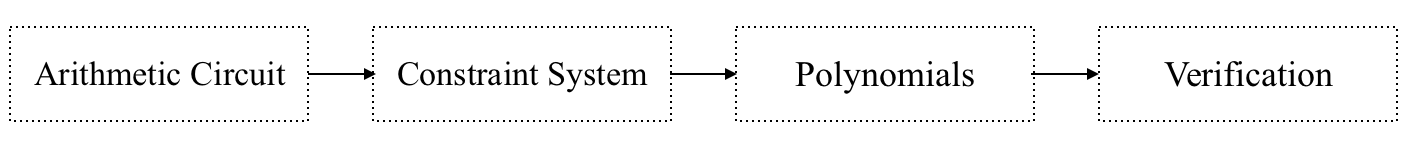
\includegraphics[width=0.8\textwidth]{Pictures/plonk_process.png}
	\caption{\acrshort{plonk} steps (simplified)}
	\label{fig:plonk}
\end{figure}

Like circuit-specific \acrshort{zksnark}s, e.g., Groth16, the computation must be flattened for the protocol to process it. The problem is represented in an arithmetic circuit consisting of gates that can represent an addition or a multiplication. Then, the arithmetic circuit is transformed into a constraint system representing the circuit's wires. In analogy to circuit-specific \acrshort{zksnark}s, the constraint system depends on the number of gates (Chapter 5.2). In \acrshort{plonk}, the constraint system is normalized into a specific form, which will be presented shortly, and is referred to as part of the public input in \citet{PLONKcryptoeprint:2019/953}. 
It is distinguished between constraints per gate and across gates within arithmetic circuits. The formalization system of gate constraints is the following:

\begin{align}
    Q_{L}a + Q_{R}b + Q_{O}c + Q_{M}ab + Q_C = 0
\end{align}

\(L, R, O\) represent the left, right, and output gate wires. \(M, C\) stand for multiplication and constant. This standardized form allows the representation of addition and multiplication. Setting \(Q_{M}ab = 0, \ Q_C=0, \ Q_{O}c = -1 \) and the rest to 1 will represent \(a + b - c = 0\). Setting \(Q_{L}a =1,\ Q_{L}b =1,\ Q_{O}c = -1\) and the rest to 0 will represent multiplication. Each gate is represented in the form presented in 5.1. Similar to the \acrshort{r1cs} previously described, \(Q_{L}a, Q_{L}b, Q_{O}c, Q_{M}ab, Q_C\) can be expressed as vectors that hold the circuit structure. Again, in analogy with the \acrshort{r1cs}, \(a, b, c\) can also be expressed as vectors, which are the witness assignments. In correlation to Chapter 4.2.1 on circuit-specific \acrshort{zksnark}s, these witness assignments might be private and only known to the prover.
In this constraint system, there are vectors \(Q_{L}, Q_{O}, Q_{M}, Q_C, a, b, c\). Using the indices of these vectors as x, they can be transformed into polynomials of evaluation format. For example, let us define one of the vectors in a circuit with 4 gates to illustrate the procedure. 

\begin{align}
    Q_L = (1,0,1,0) \text{ converts into the set of points } {(0,1), (1,0), (2,1), (3,0)}.
\end{align}

The set of points matches a degree 3 polynomial, which can be shown in a coordinate system (Figure \ref{fig:examplepoly}). Through Lagrange Interpolation, the concrete polynomial in coefficient form can be calculated. 
\begin{figure}[hbt]
	\centering
	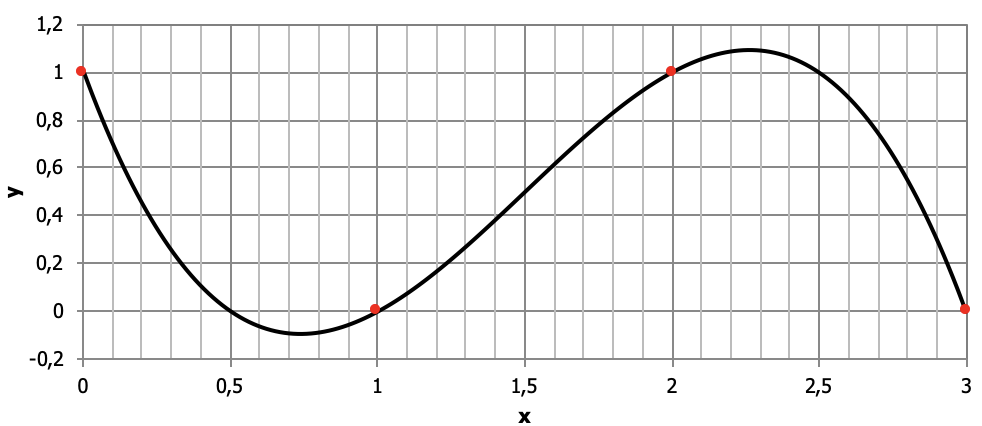
\includegraphics[width=0.6\textwidth]{Pictures/example_polynomial.png}
	\caption{Example polynomial \(Q_{L}(x)\) evaluated at the points in (4.5). Lagrange Interpolation yields coefficient form \(Q_{L}(x) = - 0.6667x^3 + 3x^2 - 3.3333x + 1\)}
	\label{fig:examplepoly}
\end{figure}

This procedure is applied to all Q-vectors and the vectors \(a,\ b,\) and \(c\) to transform them from constants into polynomials. The corresponding function obtained is
\begin{align}
    f(x) = Q_{L}(x)a(x) + Q_{R}(x)b(x) + Q_{O}(x)c(x) + Q_{M}(x)a(x)b(x) + Q_{C}(x) = 0\\
    f(x) = Z(x)H(x)
\end{align}

Now, as much information as possible can be compressed into a single source, i.e., a polynomial. 

Besides the constraints as per gate, some constraints hold across gates, e.g., the output of a gate can be equal to the input on another gate. It is necessary to represent them, too, in order to translate the whole problem into the scheme. These copy constraints can lie within one vector, e.g., if \(b0 = b2\), or between multiple vectors, e.g., \(c0 = a3 = b1\). In the first case, the indices of the vectors are exchanged to create a permutation function \(\sigma(i)\). In the second case, the vectors are combined into one long vector before obtaining the permutation function. Once all copy constraints are generated as lists of permuted indices, they are transformed into polynomials of the permuted gate indices. The resulting polynomials are
\begin{align}
    \sigma_{a}(x), \sigma_{b}(x), \sigma_{c}(x)
\end{align}

A proof is generated by using these permutations and computing the values of all the gates to create the polynomials of \(a(x), b(x), c(x)\). Now, an accumulator \(p(x)\) will be designed in order to represent all coordinates in the set of points between the vectors \(a, b, c\). It proves the copy constraints as follows.
\begin{align}
    p(x+1) = p(x) * (v_1 + X(x) + v_2 * Y(X))
\end{align}
\(v_1, v_2\) are random values and \(X, Y\) are polynomials per vector representing the x and y coordinates. For every copy constraint, e.g., \(a1=a3\) or \(b4=c1\), there will be a \(X(x)\) representing the x coordinates \(a,b, c\). \(X'(x)\) will be a polynomial representing the indices flips in the copy constraint. Every vector will be represented in \(p_{a}(n), p_{b}(n), p_{c}(n)\) and \(p'_{a}(n), p'_{b}(n), p'_{c}(n)\). Instead of checking each copy constraint within the same vector individually, the following multiplication check is also performed to check copy constraints across vectors at the same time:
\begin{align}
    p_{a}(n) * p_{b}(n) * p_{c}(n) = p'_{a}(n) * p'_{b}(n) * p'_{c}(n)
\end{align}
In practice, the permutation accumulators are not expressed in dependency of vector size \(n\) but through high-order roots of unity, whereby the field elements satisfy \(\omega^n = 1\). Also, all values are expressed as elements within a finite field of prime order \(p\), similar to the circuit-specific \acrshort{zksnark}s. The X coordinates are not expressed as indices dependent on vector size \(n\) but with \(omega\) and some random element \(g\) in the field.
\subsubsection{Summary}
After transforming all the constraints intro sets of polynomials, the following checks need to be performed to verify the proofs \citep{PLONKcryptoeprint:2019/953, buterinplonk, chen2022review}. These checks can be verified through the polynomial commitment scheme based on \citep{Kate2010ConstantSizeCT}. Elliptic curve points are generated randomly, similar to circuit-based \acrshort{zksnark}s, and used to evaluate the polynomials. Elliptic curve pairings allow checking whether the equations hold without revealing any generated points or polynomials. 
The equation in (4.3) is the main equation of the circuit that needs to be checked. Then, six permutation accumulator functions exist for the witness assignment vectors and their copy constraints. The equation check in (4.4) results in six rounds:
\begin{align}
    P_{a}(\omega x) - P_{a}(x)(v_1 + x + v_2a(x)) = Z(x)H_{1}(x) \\
    P_{a'}(\omega x) - P_{a'}(x)(v_1 + \sigma_{a}(x) + v_2a(x)) = Z(x)H_{2}(x) \\
    P_{b}(\omega x) - P_{b}(x)(v_1 + gx + v_2b(x)) = Z(x)H_{3}(x) \\
    P_{b'}(\omega x) - P_{b'}(x)(v_1 + \sigma_{b}(x) + v_2b(x)) = Z(x)H_{4}(x) \\
    P_{c}(\omega x) - P_{c}(x)(v_1 + g^{2}x + v_2c(x)) = Z(x)H_{5}(x) \\
    P_{c'}(\omega x) - P_{c'}(x)(v_1 + \sigma_{c}(x) + v_2c(x)) = Z(x)H_{6}(x)
\end{align}

There are constraints for the accumulator to be checked, which result from (4.7):
\begin{align}
    P_{a}(1) = P_{b}(1) = P_{c}(1) = P_{a'}(1) = P_{b'}(1) = P_{c'}(1) = 1 \\
    P_{a}(\omega^n)P_{b}(\omega^n)P_{c}(\omega^n) = P_{a'}(\omega^n)P_{b'}(\omega^n)P_{c'}(\omega^n)
\end{align}

The only program-specific polynomials that must be computed upfront are the \(Q\)-polynomials from the circuit and the \(\sigma\)-permutation polynomials. The verifier algorithm only stores commitments to these polynomials. The user inputs are the witness assignments \(a(x), b(x), c(x)\), the accumulators \(P\) from above, and the different \(H\) for every round. Although the verification is efficient, the proof size is still an area of improvement. For the implementation of \acrshort{plonk} in circom and snarkjs, see Chapter 5.3.

\subsection{FRI-STARK}
\begin{comment}
https://limechain.tech/blog/zero-knowledge-proofs-explained/
with FRI-based polynomial commitment
-does not use \acrshort{r1cs}
-fri starks
-Salleras et al 2021
\end{comment}

\subsection{Bulletproofs}
\begin{comment}
with discrete-log based polynomial commitment
- uses \acrshort{r1cs} too
- they are non-interactive,
- they are zk arguments of knowledge
- Godden et al bulletproofs
- Chung et. al bulletproof+
- Deng at al history of bulletproofs
-Salleras et al 2021
main protocols: Lipmaa, Boudot, then Groth and Coutueau, then Hybrid from Kim Lee 2019
Deng et al 2022: history of range proofs, cuproof as example
-Kim Lee 2019: overview on range proof protocols
\end{comment}

\section{Application Domains and Use Cases}
Zero-knowledge proofs have found broader implementation due to increasing interest in decentralized applications in recent years. However, despite successful research efforts in distributed ledger technology, there is only limited adoption of blockchain-based solutions outside the financial sector. One of the main challenges, pointed out by \citet{SedlmeirTransparencyChallenge}, is the need to make sensitive data visible. The high transparency of blockchain collides with preserving privacy and allowing for restricted visibility. \citet{Godden} describe it as increasing consciousness to preserve data confidentiality and ownership, which leads to the development of privacy-enhancing technologies. The literature review (\acrshort{slr} approach described in Chapter 3) shows that general-purpose zero-knowledge proofs find essential implementation in domains with enhanced privacy-preserving efforts. \acrshort{zkp} implementations can be categorized into the following application domains: identity management, data sharing and traceability, and system scaling \citep{PipeZK, chen2022review, morais2019survey}. Use cases from these application domains are clustered according to the problem domain they are attempting to solve (Table \ref{tab:domains}): (1) Electronic Voting and Government, (2) Electronic Auctions, (3) Data Queries and Traceability, (4) Electronic Healthcare, (5) Cloud Security, and (6) Rollups.

\setlength{\tabcolsep}{2ex}
\renewcommand{\arraystretch}{1.5}%
\begin{table}[ht]
	\centering
	    \caption{\acrshort{zkp}s Application Poblem Domains and Literature Selection}
		\begin{tabular}{| m{0.02\linewidth} | m{0.3\linewidth} | m{0.4\linewidth}|}
		\hline
		\textbf{} & \textbf{Problem Domain} & \textbf{Literature} \\ \hline
            1 & Electronic Voting and \newline Government & \citet{Bansod, Guo, Querejeta} \\  \hline
            2 & Electronic Auctions & \citet{LiXue, WangZhaoMu} \\ \hline 
            3 & Data Queries and \newline Traceability & \citet{Godden, XueWang}  \\  \hline
            4 & Electronic Healthcare & \citet{LuongPark, ZHENG, WangEtAl, Huangetal} \\  \hline 
            5 & Cloud Security & \citet{LiuWangPengXing, Major, Munivel, Kanagamani} \\  \hline 
            6 & Rollups & \citet{chen2022review, scalingintro, zksyncintro, buterinrollups} \\  \hline 
	\end{tabular}
\label{tab:domains}
\end{table}

\subsection{Electronic Voting and Government}
Motivated by recent developments in personal data protection laws, \citet{Bansod} present a governmental architecture based on self-sovereign identity to cope with the increasing demand to protect online personal information transactions. In this generalized scenario, users request a decentralized identifier from their digital governmental issuer, which will ask for personally identifiable information needed for administrative services, e.g., birth date, address, and tax identifier. The user only provides a zero-knowledge proof-enabled identity, e.g., the proof of being the person the user claims to be, and receives identity certificates from the e-government issuer. These certificates are encrypted and stored in a database and on-chain. When needing a service, e.g., renewing a driver's license, the user can request from service providers and provide the required certificates. The service provider can verify the certifications' hash values and digital signatures and provide the service once it holds.

Current privacy-preserving efforts in governmental biometric identification did not leave traditional cryptography yet. \citet{Guo} propose a novel approach to decrease governmental expenses and enable the scaling of the systems. A \acrshort{zksnark}s-based approach is presented, which reduces efficiency and eliminates fingerprint template disclosure. First, the fingerprint features are extracted by calculating the Euclidean distance of points collected. If the sizes of the distances match a certain threshold, the authentication is passed. This computation is being converted into a \acrshort{zksnark} friendly, polynomial computation with specific constraints that resulted from the first step. Then, this computation is transferred into a circuit, then to an \acrshort{r1cs}, and later into a \acrshort{qap} with three polynomial matrices. The trusted set-up generates proving and verifying keys via \acrshort{crs}. The prover algorithm creates the proof with proving key and private witness, and the verifier algorithm can perform the verification through elliptic curve pairing. The Groth16 algorithm was used to apply it to the biometric authentication example, which leaves improvement for disposing of the trusted set-up requirement and \acrshort{qap} computational time.

There are various implementations of electronic voting schemes using zero-knowledge proofs. \citet{Querejeta} introduce a first verifiable re-voting scheme with linear complexity. Voters are authenticated and can vote multiple times from any device with zero knowledge. Only the latest vote is counted. Adversaries can only obtain further information about the vote as the final result used for the election, even if they possess unbounded computational power. In the pre-election phase, the voting server generates voter identities at random, which are encrypted using the public key of the voting server and published to the bulletin board. The voters can receive such an anonymous identity and prove they are legitimate. Every time a vote needs to be made, the voting server must create the voting identities and the voter signs with their key so multiple votes can be allocated to a single voter. The voting server verifies the vote and publishes it as a ballot to the bulletin board. The voter can verify that the vote was put forward. \citet{Querejeta} included dummy votes into the scheme to prevent adversary attacks. The voting server casts dummy votes to hide the actual number of votes in the election. Finally, in the tallying phase, the tellers proceed and decrypt the votes in a verifiable and private manner. Interactive zero-knowledge proofs under the random oracle assumption are used to simulate proofs and turned into non-interactive proofs via Fiat-Shamir transformation.

\subsection{Electronic Auctions}
Zero-knowledge proof implementation efforts for bid e-auction schemes aim to prevent the exposure of bid information and price and protect the bidder's identity. \citet{LiXue} show that the goal can be met while using an auctioneer no longer becomes necessary. The latest bid price is hidden through Pedersen's commitment scheme, and the \acrshort{zkp} algorithm uses Bulletproofs so the bidder can prove that the new bidding price is higher than the previous price. Every participating bidder can verify it. The sealed-bid auction smart contract interacts with the blockchain by publishing the commitments and initializing the bidding process for the owner. The information about goods is also encrypted in the process, as well as the price and winning bidder. All participants verified the price and the winner without obtaining knowledge about them. This decentralized e-auction scheme ensures sealing and fairness while protecting the participants' privacy. Although there is no cost involved in engaging a third-party auctioneer, the productive cost of running such a platform remains to be explored.

Similar implementations without the use of public blockchain structures are found in \citet{WangZhaoMu}, which makes use of Hyperledger. Consortium members can use private channels for secure communication while effectively realizing the overall use of smart contracts and transaction privacy. In the endorsement process, the bidder initiates the transaction, and the client submits it to the endorsing peer. The endorsing peer simulates the transaction proposal and verifies it. The transaction is initiated in the ledger and returned to the platform. In the ordering process, the platform performs a combination of transactions and endorsements to be sent to the ordering peer. This peer puts the transactions into transaction blocks for every channel and delivers them to the committing peer. In the verification process, the committing peer verifies the transactions in the blocks, submits them to the ledger, and sends a notification to the platform. Zero-knowledge proofs manage the participants' identity and enable only authorized users to send requests to the client. Despite the promising architecture of Hyperledger Fabric, the practical adoptions can get very complex, depending on the use cases. This implementation requires more computational resources, in combination with the use of zero-knowledge proofs in particular.

\subsection{Data Queries and Traceability}
Protected data sharing, securing data queries, and corresponding outputs have become increasingly important during the \acrshort{covid} pandemic. \citet{Godden} propose Circuitree, a \acrshort{zkp}-based tool that can exchange verified information in zero-knowledge and implement the example of digital \acrshort{covid} certificates. The underlying query language is Datalog. A Datalog verifier is presented, which verifies each logical querying step in the reasoning process. This zero-knowledge Datalog engine is fed with domain-specific sets of rules, e.g., vaccination, test, and recovery data. The verifier, e.g., the restaurant with specific entry rules during the \acrshort{covid} pandemic, creates this rule set in Circuitree. The prover, e.g., a vaccinated person, declares their facts to Circuitree and signs them. It builds the tree-like \acrshort{r1cs} structure, converted into a bulletproof-based system. The prover can create the proof by querying the Datalog engine and, e.g., providing it to the restaurant for admission.

The problem of missing privacy preserving traceability for product development and supply chain data is being addressed in \citet{XueWang}. Parties in the industrial product development sphere can track product development history without trusting each other. There are three main layers to the newly-proposed process architecture. The traceability application layer authenticates data owners and interacts with a third party, the traceability agent. The data privacy layer, which contains the zero-knowledge proof implementation, generates traceability features in zero-knowledge and interacts with the traceability data providers, e.g., another partner in the production process inquiring about tracing some data on a specific product. The data traceability request is processed to create proof via a smart contract. The data owner acts as a verifier of this proof. The traceability features and use of the smart contract happen in the physical data layer and are mainly performed by a third party. The traceability process can be entirely monitored publicly, which solves the transparency problem in the industry while preserving the traceability inquiries and adapting to the low-trust environment of the participants.

\begin{comment}
- Fang, Near, Darias, Zhang 2021
- Xue and Wang: traceability use case applicable to pred. maintenance problem
- FAFALIOS YANNIS TZITZIKAS: link traversal, SQL
- zero knowledge static program analysis: proof that a secret code is correct (Fang, Near, Darias, Zhang 2021)
\end{comment}

\subsection{Electronic Healthcare}
Patient monitoring nowadays is increasingly remote, i.e., health data collection happens via medical devices. \citet{LuongPark} uses \acrshort{zksnark}s to enable patient medical data sharing between medical devices and health service providers. The main interactions happen between the patient, medical device, and health service provider. The health service provider is responsible for collecting patient data from the medical device, analyzing it, and responding with adapted features and enhanced functions in the medical device provided. The patients initialize the process using their public address in the blockchain system and creating signed hashes. The provider uses these hashes to create an arithmetic circuit and initiate the \acrshort{zksnark}s protocol. Parameters and the zk-proof are created via a smart contract. Patients can use the smart contract to authenticate themselves and add additional information, e.g., the device. Through a secure key exchange algorithm, the health service provider can share encrypted patient data with medical devices via a secure, zero-knowledge communication channel. The underlying \acrshort{zksnark}s used is Pinocchio \citep{Pinocchio}, implemented via Zokrates \citep{ZoKrates}. Even though the proof generation takes a long and the system is not suitable for mobile devices due to the nature of the tools used, it solves current problems due to the lack of anonymous and secure patient data sharing between medical devices and health service providers, e.g., adversary attacks and unauthorized disclosure of health data.

Efforts for patient health data privacy protection also reach the medical insurance purchase and claim process, as underlined by \citet{ZHENG} and \citet{WangEtAl}. Health data is shared securely, and the patient's identity is disclosed to a minimum using non-interactive zero-knowledge proofs. Patients provide their health data in a regulated and authenticated manner via smart contracts. Hereby, the hospital acts as a fully trusted data generator, interacting with the smart contract. Patients can obtain medical data from the hospital, providing a unique identity. The insurance companies publish their restrictions and requirements, e.g., for purchasing medical insurance, via smart contracts on-chain. The hospital uses these requirements to build the constraint system and circuit and produce a proof alongside the encrypted medical data and patient identity. The medical insurance company can verify this proof, and the smart contract can initiate purchasing or claiming between the patient and insurance company without compromising patient identity and sensitive health data insights. Other peers in the blockchain verify the validity of the payment transaction.

In contrast to the increasing consciousness about data protection and excessive amounts of patient data available, there is a need to process medical data effectively to enable research and health care. Implementations of \citet{Huangetal} try to leverage these opposites by implementing secure medical data sharing between patients, health care providers, research institutions, and semi-trusted servers on the cloud. It is achieved using a private blockchain in Hyperledger Fabric combined with \acrshort{zksnark}s. Research institutions put their requirements for medical data, e.g., study inclusion criteria, into an arithmetic circuit and publish a proof. Patients encrypt their medical data independently or can authorize their health care provider, e.g., hospitals. The encrypted and signed medical data is sent to the semi-trusted cloud server and broadcasts the encrypted data on-chain. Whenever patients decide to share their medical data with research institutions, another proof has to be created to show that the medical data matches the research institution's research criteria. It is achieved via smart contracts and the proof algorithm specified there. It also verifies this proof, and upon success, the patient can generate the re-encryption key used in conversion to the public key of the specific research institution. The cloud server receives this re-encryption key and signs it on top with its public key. This enables the research institution to decrypt the medical data, while the semi-trusted cloud server cannot obtain further knowledge. It is captured in a transaction that participating nodes in the network can verify via consensus.

\subsection{Cloud Security}
Robust authentication schemes for client and user authentication on cloud servers experience enhancement due to the increasing practical applicability of zero-knowledge proofs. Implementation efforts of \citet{LiuWangPengXing} show how a center-less and biometric-based single sign-on across cloud services can work. The user gets registered in the registration center, which does not participate another time in the authentication procedure, which removes centralization vulnerabilities. A token service provider generates a zero-knowledge token for the user, which is used across multiple cloud services. The underlying technology is based on circuit-specific \acrshort{zksnark}s, e.g., Groth16. An elliptic curve over a finite field with generator points is used, and a common reference string is issued, whereby the token service provider performs the set-up phase. The user adds secret values, i.e., user identity, password, and biometric information, as secret values. The token service provider registers the user and delivers a token without learning the decrypted user's secret values. The cloud service provider also registers via the token service provider. Each registration ends with a zero-knowledge token provision. The user and cloud service provider verify each other, whereby a specific session key is generated. This session key authenticates the user on other cloud service providers.  

In \citet{Major}, a prototype applies zero-knowledge proofs for lightweight and private client-server authentication based on port knocking. Port knocking is widely used as an authentication mechanism between clients and firewalls, allowing for a channel between them within an untrusted network, e.g., the Internet. The host authenticates the client without open ports, and attacks are difficult because the machine's function as a server is hidden. Non-interactive zero-knowledge proofs are used in the prototype to work towards the goal of hiding any further knowledge from sniffing traffic or eavesdropping. In the set-up phase, profile files for the client and server are created, whereby only the client has a secret private key in the file, which is randomly selected.
Furthermore, the files contain the parameters for the \acrshort{zkp}, a private hash key, the server port number, and the command to be run upon successful authentication, e.g., to mount an app service. The client creates the proof, treats it like the knock, and transmits it to the port-knocking server. The server parses the traffic, inspects it, and checks whether \acrshort{zkp} criteria are met, e.g., that the server port specified by the client matches. If the checks are met, the protocol is executed further to perform the computational verification through bilinear pairings. If the verification passes successfully, the client-specific command can be executed.

Password attacks have increased, especially observing the rising usage of cloud storage services for mobile devices. This threat is analyzed in \citet{Munivel}, and a new authentication scheme is proposed using zero-knowledge proofs for mobile cloud storage authentication. The client server provides a unique in-browser mask for entering user identifier and password. In the background, these values are hashed and do not leave the browser as entered with the user's public key and a random value, which is an element of a cyclic group of prime order. The user's algorithm calculates a proof consisting of a random token, the password hash hidden by some generator from the cyclic group and the random value, and the user's public key. The server calculates the verifying key, and, i.e., similar to the circuit-specific \acrshort{zksnark}s verify algorithm, can check whether the proving information sent by the user matches. The server can do this because the server has access to the random token, user public key, and the group element generator, which are public elements. Neither the server nor an adversary can obtain the user password and receive access to the cloud storage.

Apart from research on cloud authentication, there are implementation efforts to use zero-knowledge proofs for storing only one single copy of the same data on cloud servers, i.e., data deduplication efforts. Motivated by mass data storage outsourcing to third-party cloud computing providers, data deduplication and dynamic ownership are promising areas of development. On the assumption that the cloud server is honest but curious, \citet{Kanagamani} propose a data deduplication scheme using in-line block matching and interactive zero-knowledge proofs. The cloud server performs the deduplication check by verifying the proof of ownership of the file and checking whether a copy is already stored while learning no further information about the ownership and the file. Before the initial upload, the file should have been hashed already. The server registers users and provides them with public and secret keys. The encryption key is obtained by applying another hashing algorithm to the file hash.
Further, this key is hashed once more to obtain the tag. The cloud server refers to the tag to check whether a subsequently uploaded file already exists. The user chooses a random encryption key, which is different, and encrypts the encryption key to obtain a ciphertext. The tag, ciphertext, user identifier, and the proof are stored in the cloud server. The proof is obtained by combining in-line block matching with zero knowledge proof generation. The file is divided into blocks, and each block is used to perform an exponential equation with some primes \(a\) and calculated in modular arithmetic with another prime \(mod \ b\). All computations are performed using a multiplicative cyclic group \begin{math} \mathbb{G} \end{math} with prime order \(t\). The result of each calculation forms a sequence of individual block proofs, which are the file proof. The server receives the proof and the data described above and checks if the tag matches any other tag of a file stored previously. Group keys are generated for verification and used to perform bilinear pairing checks, i.e., similar to \acrshort{zksnark}s, e.g., Groth16. The public key of the file is taken alongside random prime numbers to obtain the group key. The ciphertext is encrypted with the group key by the server and stored with the ownership information. Each time the ownership changes, the server uses the existing proofs to send challenges to the allegedly new owner. The new owner responds by creating secret values from the challenge received. Once the server can verify the proof, secret, and response, another group key is generated and used to encrypt the ciphertext of the file. The ownership information can be changed. The server learned nothing more than a change in ownership and that the file only existed once. 

\subsection{Rollups}
Implementing zero-knowledge rollups enhances the throughput of blockchain transactions through outsourcing computation off-chain and only performing the validation part on-chain. Often referred to as validity rollups, they do not show the property of perfect zero-knowledge. In this reflection, only application-specific rollups are discussed. General rollups, e.g., Zcash and Tornado Cash, are not in scope (Chapter 3). In application-specific rollups, the most expensive part of the blockchain application is deployed via rollups. All rollups in practice can be categorized into validity-style rollups and validium-style rollups \citep{chen2022review}.

Along with the scope of application-specific implementations, Ethereum is the most widely used Turing-complete blockchain to build apps. However, the block validation time of 15 seconds per block results in significantly high gas cost, and with increasing volume, Ethereum can barely serve the number of users \citep{scalingintro}. The general idea of rollups is to solve this via off-chain computation of transaction states \citep{chen2022review}. In order to realize it, another blockchain layer (L2) is utilized. The main layer (L1) deploys a smart contract, which interchanges tokens with L2 and verifies that computations and transactions on L2 are performed correctly. In an Optimistic Rollup, the L2 scaling is approached with the assumption that every transaction is valid until proven invalid. It depends on users to submit proofs to claim that some transaction was forged to ensure transaction security \citep{zksyncintro}. Zero-knowledge rollups are different because the rollups smart contract verifies each transaction state transition before it becomes effective. 

Validity-style rollups follow the following architecture \citep{buterinrollups}: validators on the mainnet bridge between L1 and L2, receiving submitted transactions by users who signed their transaction activities on L2. These validators perform the following scaling procedure: all submitted transactions are scaled, i.e., aggregated, into a single batch and submitted to the L1 smart contract for further processing. In essence, the L2 state root, a \acrshort{zksnark} to prove L2 state root correctness, every transaction header, and the Merkle root of the transaction batch are submitted to the smart contract. In L1, the validation of the entire batch and the suggested update of the Merkle state root can be performed. First, batch verification is more inexpensive. Second, the off-chain storage of the state root increases the performance on the mainnet, boosts its capacity, and decreases transaction fees \citep{chen2022review}. In validium-style rollups, the transaction header is not stored and provided; instead, the \acrshort{snark} proves the validity of the state transition. Because of this, validium-style rollups are additionally perceived as proof of knowledge, whereas validity-style rollups only serve as proof of computation \citep{validiumintro}. 

\begin{comment}
-start with zk Roll ups, sources: Chen et al (2022): very good overview on rollups, validium, zkEVM with TinyRAM, recursive SNARK by MatterLabs

good implementation papers:
- Xu Chen(2021)-->Seite 307 in GoodNotes: new algorithms for zero knowledge set membership for ZK-scaling, based and compared to zkSync
-Soonhyeong 2021: better verification with EVM to verify non-maliciousness of blocks (zKSNARKS used)
-Yang, Weng, Sarkar, Wang: memory effieciency enahncements

\end{comment}

\section{Evaluation and Challenges}
As presented above, \acrshort{zksnark}s are successfully implemented in various application scenarios, but weaknesses remain to be discussed. The zero-knowledge proofs presented earlier are contrasted to condense differences and similarities. Ultimately, the main challenges of trust assumption, cost, and quantum computing are summarized in this chapter, providing an outlook on future solution approaches currently discussed in the research.

Zero-knowledge proof evaluation approaches can be grouped into computational complexity analysis \citep{LiuWangPengXing, SONIC10.1145/3319535.3339817, PipeZK}, security analysis \citep{Huangetal}, and communication cost \citep{ZHENG, liuetal, gongetal}. This subchapter compares specific aspects of these categorizations. First, highlighted characteristics of \acrshort{zksnark}s, \acrshort{zkstark}s, and Bulletproofs are revisited. Second, the analysis aspects of trusted set-up, communication complexity, and quantum threat are emphasized. 

The cryptographic assumption of \acrshort{zksnark}s is secure bilinear pairings with a short proof length and smaller memory consumption on-chain. However, a trusted set-up with a \acrshort{crs} is needed. A third party generates the proving and verifying key. A multi-party ceremony (\acrshort{mpc}) can diffuse the centralization of trust by letting hundreds of participants generate the \acrshort{crs} \citep{liuetal}. Zk-STARKS have a faster verification and proof speed. The larger proof and circuit size (bytes versus several hundred kilobytes) make \acrshort{zkstark}s more complex than \acrshort{zksnark}s. There is no necessity for a trusted set-up and \acrshort{crs} because of the hash collision-based symmetric encryption, which is free from arguments of knowledge; thus, \acrshort{zkstark}S are not vulnerable to quantum computers. Bulletproofs do not need a trusted set-up and possess a logarithmically increasing proof size. There is good applicability with range proofs and short proof sizes for general arithmetic circuits, although bulletproofs are faster to be verified than range proofs \citep{gongetal}. Unlike all other \acrshort{zkp}s discussed in this chapter, bulletproofs enable efficient on-chain proof storage. 

The \acrshort{crs} generated in \acrshort{zksnark}s relies on a third party. Zk-STARKs utilize verifiable randomness, which makes a \acrshort{crs} obsolete. Bulletproofs can avoid a trusted set-up because of the discrete logarithm assumption and a completed 128-bit security in untrusted environments \citep{Huangetal}. The communication complexity in \acrshort{zksnark}s grows nearly linear in \(O(1)\) because the prover hands over the proof to the verifier while the computational workload increases. Zk-STARKs have the largest run time with poly logarithmic functional expressions, with \(N\) being the input size of the circuit (Table \ref{tab:complexity}). In Groth16, the prover complexity can also be described as \(m + 3n - l*E\), with \(m\) circuit wires, \(n\) multiplication gates, \(l\) elements in the statements, and \(E\) exponentiation operations \citep{Groth2016OnTS}. Zk-STARKs possess the highest computational efficiency in proof and verifier complexity \citep{gongetal}.
\setlength{\tabcolsep}{2ex}
\renewcommand{\arraystretch}{1.5}%
\begin{table}[ht]
	\centering
	    \caption{Complexity Comparison of \acrshort{zksnark}s, \acrshort{zkstark}s, and Bulletproofs}
		\begin{tabular}{| m{0.15\linewidth} | m{0.2\linewidth} |              m{0.2\linewidth}      | m{0.2\linewidth}|} \hline
		\textbf{} & \textbf{\acrshort{zksnark}s} & \textbf{\acrshort{zkstark}s} &\textbf{Bulletproofs}       \\ \hline
            Prover \newline complexity & \(O(N*log(N)\) & \(O(N*log(N)^k)\) & \(O(N*log(N)\) \\  \hline
            Verifier \newline complexity & \(O(1)\) & \(O(log(N)^k)\) & \(O(N)\) \\ \hline 
            Proof size & \(O(1)\) & \(O(log(N)^k)\) &  \(O(log(N))\)\\  \hline
            Post-quantum security &  not given & given & not given\\  \hline 
	\end{tabular}
\label{tab:complexity}
\end{table}

Even though quantum computers are not fully mature yet, it is a considerable threat to be discussed when evaluating zero-knowledge proof algorithms. The quantum threat to \acrshort{zkp}s comes from their ability to break encryption algorithms, which threatens blockchain security.

\acrshort{zksnark}s are easy to be broken by quantum computers due to the ability of quantum machines to break polynomial evaluation. It has yet to be discovered how \acrshort{zkstark}s can be broken by quantum computing due to collision-resistant hashing functions (for \acrshort{ip} and \acrshort{rom}). Bulletproofs rely on discrete logarithm assumptions for problem-solving, which makes it particularly easy for quantum computers to break. The commitment values are exposed by adversaries \citep{gongetal}. 

Recalling from the definition of quantum zero-knowledge (QZK) introduced by \citet{watrousqzk}, various approaches enhance classic zero-knowledge proofs to become quantum secure. In QZK, the verifier \(V\) could be quantum, i.e., for any polynomial-time quantum verifier, there exists a quantum simulator \(S\), such that any mappings induced between them are quantum computationally indistinguishable. Even though there could be a quantum verifier, it should not obtain knowledge. All approaches to obtain quantum resistance focus on specific classic properties of zero-knowledge proofs and transform them to be suitable against quantum adversaries. For example, security notions of witness indistinguishability (WI) and witness hiding (WH) are studied to construct the quantum variants of those, and ultimately, propose a quantum secure signature scheme to construct the \acrshort{crs} \citep{xieyang2019, katzetal}. WI refers to a proof system in which the verifier cannot know which witness was used by the prover. WH describes the verifier's inability to compute the unknown witness through interaction with the prover. \citet{Vidick2020classicalzero} construct a zero-knowledge protocol sound against polynomial-time quantum provers and both classic and quantum polynomial-time verifiers. It uses a perfect binding, quantum computationally concealing commitment protocol with extended trapdoor functionalities. Another approach to construct QZK focuses on the \acrshort{mpc}, providing quantum secure digital signature algorithms based on asymmetric key primitives, e.g., ZKBoo and ZKB++ \citep{gongetal}.

Recursive SNARKs is a promising research field when discussing the future of ZK. With \acrshort{zksnark}s, proving the correct execution of a specific multi-step function at a given step requires the computation of each step, which can be improved. For example, not all function steps are known, computing all these steps is computationally too expensive for the use case, or it is not efficiently feasible to process all proofs if the amount of participating provers is high. Recursive \acrshort{snark}s act as aggregators so that \acrshort{snark}s can be applied for each iteration to prove the correctness of a previous proof \citep{chen2022review}.

\begin{comment}
%polylog : https://crypto.stackexchange.com/questions/48638/whats-the-difference-between-polylogarithmic-and-logarithmic

trusted set-up:
- \acrshort{crs} is relied on in zksnarks and third party needed
- no \acrshort{crs} required in zkstarks because verifiable randomness is utilized 
-bulletproofs avoid trusted set-up because of discrete logarithm assumption and completed 128-bit security in untrusted environment 

complexity analysis: algorithmic complexity of communication (proof size), prover and verifier:
algorithmic complexity: 
communication complexity: 
- zksnarks almost in linear o(1), because prover hands proof over to verifier, while computational workload increases significantly
prover complexity:
-starks the fastest with polylog, however they have largest proof size (polylog n)
-snark: O(NlogN) with N input size of the circuit
%-->groth16 paper:m + 3n −l*E with circuit of m wires, n multiplication gates, l elements in the statements and E exponentiations (Gro16 paper source)
%https://hackernoon.com/trade-it-like-it-is-hot-a-review-of-popular-zk-projects-and-the-zero-knowledge-proof-technology
%https://www.alchemy.com/overviews/snarks-vs-starks
%https://consensys.net/blog/blockchain-explained/zero-knowledge-proofs-starks-vs-snarks/
verifier complexity:
-zk-snarks: O(1), one verification step, in Groth 16 consisting of 3 pairing checks
-zk-snarks faster verifier than zk starks
- polylog faster than log base 2
quantum threat:
- only starks are quantum secure



\section{Evaluation Methods}
-Huang et al 2020: 1)privacy preserving and security: confidentiality, availability, integrity, privacy-preserving, traceability, single point of failure 2) performance evaluation: computing cost, number of startup nodes, privacy protection, time to generate NIZK keypair, NIZK proof, verify NIZK proof
-Zhang et al 2021 PipeZK proof generation enhancement
- Maller et al 2019 Sonic: better structured SRS in linear size to speed up proof verification
- Chen et al (2022): future of ZK are zk-STARKS
\subsection{Performance Analysis}
-Liu et al, Zheng at al: semihonest model evaluation topics-> computational complexity, communication complexity, experimental evaluation
- Liu Wang Peng Xing 2019: remote authentication for mobile cloud computing, Real-Or-Random model and BAN logic for security evaluation REGARDING different attacks
- Zhang et al 2021 PikeZK: new hardware accelerator to boost comp time for proof generation


- challenges can go into evaluation/comparisons of the 4 zkps
\subsection{Cost}
-Zhang et al 2021 PipeZK time and cost challenges of zKSNARK
-effieciency of ZKP: computation depends on field size-->there is a need for memory efficient ZKPs: wolverine and mac'n'cheese can do it better, but QuickSilver better protocol for large circuits (Yang, Weng, Sarkar, Wang 2021), Dittmer et al (2022) outperform Quicksilver then (most current best performing memory based protocol)
-elements from Sedlmeier Völter Strüker (2021): take the cost of Groth16

\subsection{Trust Assumption}
-Huang et al 2020 semi trusted proxy server, their assumptions
-trusted set up for zk Snarks

\subsection{Quantum Computing Threats}
1. Why are quantum verifiers a threat? (maybe Katz et al 2018)
2. different aspects of solution examples
-Deng et al 
- Xie Yang 2019: quantum secure CRS, good arguments of other shortcomings of ZKP systems, interactive and non interactive quantum zero knowledge proof systems
- Vidick Zhang 2020: describe the three problems that there are protocols developed for (big umbrella problem: quantum verification problem), good definitions from the quantum world
- also include Watrous(2009)-->coming from Vidick Zhang 2020
-Lyubashevsky et al (2020): new lattice based ZKP algorithm which is the fastest and smallest proof size for small int addition and multiplication 

\subsection{Sustainability}
-maybe too little literature for an own sub chapter
-Simunic et al mention need for more sustainable solutions in blockchain privacy preserving through ZKPs32
-elements from Sedlmeier Völter Strüker (2021): ZKPs are more sustainable 

    end this chapter with (maybe):
    - ZKPs still need more practical implementations and adoption in real life use cases
    - main problem is black box appearance of ZKPs and lack of awareness on how they can be leveraged and when does what work in specific scenarios and on what conditions
\end{comment}

\begin{comment}
     -->future of snarks in chapter 6 of chen et al
    - quick excurse to starks and recursive snarks being the future
    - damit hätte ich dann trust assumption abgedeckt!
    - tiny bit overview on why snarks are not quatum secure and what is quantum secure
   
\end{comment}

    \clearpage{\pagestyle{empty}\cleardoublepage}
    \chapter{Implementation and Results}
The following sub-chapters present the results of this master thesis. First, the requirements are summarized. Subsequently, the example computation of a Groth16 proof and verification is described in detail. The first artifact, the zero-knowledge decentralized application (\acrshort{zkdapp}), is demonstrated. The second artifact, an architecture proposal for the zero-knowledge data structure of spare part certification and metadata information, is introduced as an outcome of the \acrshort{zkdapp} evaluation.

\section{Summary of Requirements}
The requirements introduced in Chapter 2 and 3 are summarized as follows.

\begin{enumerate}
    \item Zero-knowledge proof systems are a disruptive technology in the domain of blockchain-based research and development. One project requirement is to \textbf{accumulate knowledge and current research outcomes} in this field to extend expertise within RAPADO \citep{ZedelJ}. The Groth16 algorithm is introduced in detail using an example calculation problem (Chapter 5.2). The problem is split and transformed into an arithmetic circuit in the step-wise computation, arriving at an \acrshort{r1cs}. From this, the \acrshort{qap} is calculated. Tools, e.g, homomorphic hiding and elliptic curve pairing, are also introduced. Ultimately, following the Groth16 protocol, the key and proof generation and verification mechanisms are illustrated.
    \item The requirement of \textbf{constructing a trade-off between privacy, confidentiality, and transparency} arises from preliminary work in the project and at the Department of Information Systems \citep{ZedelJ}. The use of blockchain-based solutions enables transparency at the cost of confidentiality. With the constantly increasing awareness for data privacy, combined with trust issues and regulatory data confidentiality requirements in the industry, zero-knowledge proof systems have to be explored and utilized to secure the adoption of project results and products in the future. The first minimum viable product (MVP) of the \acrshort{zkdapp} for \acrshort{mro} data attestations contributes to this goal and satisfies this requirement. The \acrshort{zkdapp} is organized as follows: the backend directory stores the JSON input schema, the solidity smart contracts, the circom circuit, and corresponding generated files. The lib directory stores shared files between the backend and frontend and hashing functions used, e.g., in the circuit code. The user interface (UI) directory finds the correct schema and stores a copy of the final protocol transcript key and the witness-generating file. It also stores the frontend code for the landing page and all corresponding pages to submit, attest to and verify \acrshort{mro} data.
    \item Current paper-based \acrshort{mro} documentation of aviation spare parts primarily sets the requirement for \textbf{fraud-preventive document authenticity checks, enabled through practical data formats and digitization of spare part documentation}. Fraud-preventive verification is covered via the \acrshort{zkdapp}. However, current data digitization efforts for spare part documentation need to be further addressed: the zero-knowledge data structure architecture enables consistent and temper-proof data storage via Merkle trees, and proofs specific memberships, e.g., mechanics who worked at a specific part at a given time, in zero-knowledge.
\end{enumerate}

\begin{comment}
-research disruptive technologies and creating knowledge in the project: calculation example Groth16
-privacy/confidentiality vs transparency : \acrshort{zkdapp}
-need for fraud-preventive verification mechanism enabled through effective data formats digitization of aviation parts and document data: architecture

Notizen:

In den Ausblick der \acrshort{zkdapp}
-für einen part die schwellenwerte finden
-time since last service
-validation network as attester—>Übergang zum 2.artefakt 

-schwellenwerte ausgelesen werden
-aber auch die attester müssen ausgelesen werden

—>release certificate: Behörde
—> shop report: MRO Betrieb

-MRO KPIs: für den Handel, aus den MRO Daten ergeben, aus Privatsphäre/Transparenz requirement, ohne dass man Einsicht ins gesamte shop report geben will
\end{comment}

\section{Groth16 Proof and Verification}
Let us use an example to illustrate the underlying mathematical methods applied in \acrshort{zksnark}s. The example calculation will use the knowledge of the coefficient assumption for simplification. In practice, the \acrshort{fft} is applied. First, the arithmetic circuit is transformed into an \acrshort{r1cs}. The \acrshort{r1cs} is used to obtain the \acrshort{qap}. Homomorphic hiding, elliptic curves, and pairing-based cryptography are introduced in more detail and put in context for the next steps of the calculation. Finally, the Groth16 protocol is introduced: First, the key generation steps are explained. Second, the proof is generated. Lastly, the verification steps are illustrated. Formal definitions are found in Chapter 4.2.

Say we want to prove we know a secret x so that

\[x^3 + x + 5 = 35\]

In this case, our secret is x = 3.
In practice, we would use hiding and modular arithmetic instead of real numbers and calculations since these are easy to forge and find solutions to, making the proof useless. For the \acrshort{r1cs} and \acrshort{qap}, we will proceed with real numbers to show the underlying mechanisms. The following will demonstrate how any computation that needs to be proven can be converted into polynomial format.

\subsubsection{Arriving at a R1CS}

A rank-1 constraint system is a mathematical format to help us reduce our problem into a less complex computational problem. First, we flatten the equation by writing a short program to break down the different steps to solve the equation.

\begin{enumerate}
    \item \(sum1 = x * x\)
    \item \(y = sum1 * x\)
    \item \(sum2 = y + x\)
    \item \(out = sum2 + 5\)
\end{enumerate}

As shown above, we arrive at an arithmetic circuit with 4 gates and the solution variables
\[x = 3, y = 27, sum1 = 9, sum2 = 30, out = 35.\]

From this, we can construct the solution vector \(s\), starting with a dummy variable of value 1, which we call \textit{one}.
Now, the solution vector \(s\) is
\begin{align}
    \Vec{s} &= \begin{pmatrix}
     one \\ x \\ out \\ sum1 \\ y \\ sum2
\end{pmatrix}
\end{align}
Each gate will be represented so that
\begin{align}
     \Vec{s}\cdot\Vec{a_i} * \Vec{s}\cdot\Vec{b_i} - \Vec{s}\cdot\Vec{c_i} = 0
\end{align}

Let us go through every gate and assign the values for \(a, b,\) and \(c\).
For the first gate \(sum1 = x*x\), the values of \(a, b,\) and \(c\) are assigned as follows:
\begin{align*}
    a_1 &=\begin{bmatrix}
        0 & 1 & 0 & 0 & 0 & 0
    \end{bmatrix}
\end{align*}
\begin{align*}
    b_1&=\begin{bmatrix}
        0 & 1 & 0 & 0 & 0 & 0 
    \end{bmatrix}
\end{align*}
\begin{align*}
    c_1&=\begin{bmatrix}
        0 & 0 & 0 & 1 & 0 & 0
    \end{bmatrix}
\end{align*}

The above is correct because the dot product of s and a, multiplied by the dot product of \(a\) and \(b\), subtracted by the dot product of \(s\) and \(c\), is 0.

This procedure is applied to every gate. Let us show more complex gates to underline the calculation. For example, the third gate and the fourth gate. The third gate \(sum2=y+x\) could be approached as the first gate by setting the variables in the equation to 1. However, this would not fulfill the equation shown in (5.2). Therefore, the correct values for \(a_3, b_3 \text{ and }c_3\) are
\begin{align*}
    a_3 &=\begin{bmatrix}
        0 & 1 & 0 & 0 & 0 & 0
    \end{bmatrix}
\end{align*}
\begin{align*}
    b_3&=\begin{bmatrix}
        1 & 0 & 0 & 0 & 0 & 0 
    \end{bmatrix}
\end{align*}
\begin{align*}
    c_3&=\begin{bmatrix}
        0 & 0 & 0 & 0 & 0 & 1
    \end{bmatrix}
\end{align*}

Here, we make use of the dummy vector \textit{one} so that we can arrive at 
\[30 * 1 - 30 = 0.\]

The fourth gate \(out=sum2+5\) must also be approached by holding to the dot product equation in (5.2). We have to make use of the dummy vector once again. Setting the values of \(one, sum2 \text{ and } out\)  to 1 will give us the following incorrect solution:
\begin{align*}
     \Vec{s}\cdot\Vec{a_4} * \Vec{s}\cdot\Vec{b_4} - \Vec{s}\cdot\Vec{c_4} \neq 0.
\end{align*}
The calculation shows \(30 * 1 - 35 \neq 0\), which means we need to add 5 so that the dot product of vector \(s \text{ and } a\) adds up to 35. Therefore, the values of \(a_4, b_4 \text{ and }c_4\) are as follows:
\begin{align*}
    a &=\begin{bmatrix}
        5 & 0 & 0 & 0 & 0 & 1
    \end{bmatrix}
\end{align*}
\begin{align*}
    b&=\begin{bmatrix}
        1 & 0 & 0 & 0 & 0 & 0 
    \end{bmatrix}
\end{align*}
\begin{align*}
    c&=\begin{bmatrix}
        0 & 0 & 1 & 0 & 0 & 0
    \end{bmatrix}
\end{align*}

By combining our results into matrices, we can set up the corresponding \acrshort{r1cs}:

\begin{align}
A&=\begin{pmatrix}
    0 & 1 & 0 & 0 & 0 & 0 \\
    0 & 0 & 0 & 1 & 0 & 0 \\
    0 & 1 & 0 & 0 & 1 & 0 \\
    5 & 0 & 0 & 0 & 0 & 1
\end{pmatrix}
\end{align}
\begin{align*}
B&=\begin{pmatrix}
    0 & 1 & 0 & 0 & 0 & 0 \\
    0 & 1 & 0 & 0 & 0 & 0 \\
    1 & 1 & 0 & 0 & 0 & 0 \\
    1 & 0 & 0 & 0 & 0 & 0
\end{pmatrix}
\end{align*}
\begin{align*}
C&=\begin{pmatrix}
    0 & 0 & 0 & 1 & 0 & 0 \\
    0 & 0 & 0 & 0 & 1 & 0 \\
    0 & 0 & 0 & 0 & 0 & 0 \\
    0 & 0 & 1 & 0 & 0 & 0
\end{pmatrix}
\end{align*}

\subsubsection{From \acrshort{r1cs} to \acrshort{qap}}

The \acrshort{r1cs} shows three matrices \(A, B \text{ and }C\) representing the four gates of length six. It is transformed into a \acrshort{qap} by expressing polynomials as sums of Lagrange Interpolation (Chapter 4.2.1). This results in three sets of polynomials \(A_i(X), B_i(X) \text{ and }C_i(X)\), each consisting of six polynomials of degree three. In the following, we will summarize the reason for setting up a \acrshort{qap} instead of continuing with the \acrshort{r1cs}. Lagrange Interpolation allows us to develop polynomial coefficients representing each gate when evaluated at an \(X\) in the range of the number of constraints (gates). With \(X = 1\), the Lagrange Interpolation can be explained quite well because it means that we can add up the coefficients of the polynomials in \(A_i(X), B_i(X) \text{ and }C_i(X)\). Each set of polynomials is built so that evaluated at gate \(X\), whereby \(X\) has to be in the range of the number of gates (constraints), will deliver the specific value of \(X\) and 0 for the other values in that specific range.\newline
The \acrshort{qap} for our example:
\begin{align*}
    A_i(X) \\
    \begin{bmatrix}
        -5.0 & 9.166 & -5.0 & 0.833 \\
        8.0 & -11.33 & 5.0 & -0.666 \\
        0.0 & 0.0 & 0.0 & 0.0 \\
        -6.0 & 0.5 & -4.0 & 0.5 \\
        4.0 & -7.0 & 3.5 & -0.5 \\
        -1.0 & 1.833 & -1.0 & 0.166
    \end{bmatrix} \\
\end{align*}
\begin{align*}
        B_i(X) \\
    \begin{bmatrix}
        3.0 & -5.166 & 2.5 & -0.333 \\
        -2.0 & 5.166 & -2.5 & 0.333 \\
        0.0 & 0.0 & 0.0 & 0.0 \\
        0.0 & 0.0 & 0.0 & 0.0 \\
        0.0 & 0.0 & 0.0 & 0.0 \\
        0.0 & 0.0 & 0.0 & 0.0
    \end{bmatrix}
\end{align*}
\begin{align*}
        C_i(X) \\
    \begin{bmatrix}
        0.0 & 0.0 & 0.0 & 0.0 \\
        0.0 & 0.0 & 0.0 & 0.0 \\
        -1.0 & 1.833 & -1.0 & 0.166 \\
        4.0 & -4.833 & 1.5 & -0.166 \\
        -6.0 & 9.5 & -4.0 & 0.5 \\
        4.0 & -7.0 & 3.5 & -0.5
    \end{bmatrix}
\end{align*}
The corresponding values in the matrices represent polynomial coefficients and shall be read from right to left, e.g., \(A1(X) = 0.833x^3 - 5x^2 + 9.166x -5\). For example:
\begin{align}
     X = 1 \\
    A1(1) = 0, A2(1) = 1, A3(1) = 0, A4(1) = 0, A5(1) = 0, A6(1) = 0
\end{align}
Comparing the results with the first vector \(a\) of the first gate, we see that the results represent the first gate.
For example, evaluating \(A, B \text{ and }C\) at \(X = 1\) means adding up the coefficients of the first polynomial of \(A\), which will result in a value matching to the vector value in the first gate. Then, the next polynomial in A, etc. It will result in a vector of length six and be correct if the values match vector a from the first gate in our \acrshort{r1cs}. The same is done by evaluating the polynomials with \(X\), whereby \(X\) starts at \(1\) and ends at the number of gates, in our case \(X=\{1,2,3,4\}\).
However, it would be cumbersome to evaluate each constraint individually. This is why we can make use of the \acrshort{qap} to check whether the dot product equation of the polynomials will hold:
\begin{align}
    A_i(X)\cdot \Vec{s} * B_i(X)\cdot \Vec{s} - C_i(X)\cdot \Vec{s} = H(X) * Z(X)
\end{align}
Interestingly, the left side of the equation is our target polynomial \(T(X)\), which we want to prove.
Now, look at the equation's right side in (5.6). \(Z(X)\) is known if we know the number of constraints. In Groth16, it is made available in the trusted setup. In this case, we have four gates, so we arrive at
\begin{align}
    Z(X) = (x-1)(x-2)(x-3)(x-4)
\end{align}
\(H(X)\) is the hiding of our initial minimal example, those inputs we do not want to share but prove we know the solution. What role hiding plays will be explained shortly. We want to finish looking at the equation in (5.6). In essence, we want to prove that we know a polynomial and its solution so that
\begin{align}
    T(X) / Z(X) = H(X)
\end{align}
In our example, \(H(X)\) is also a polynomial. The \acrshort{qap} is correct if \(H(X)\) is a polynomial without remainder. In this example, the resulting
\[H(X) = -0.44x^3 + 17.055x^2 - 3.666x.\]

Practically, the coefficients of each polynomial in \(A_i(X), B_i(X) \text{ and }C_i(X)\) are publicly known. The same can be said for \(Z(X)\) through knowing the number of constraints (in this example, we have four constraints). The prover can calculate the coefficients of \(H(X)\) by dividing T(X) / \(Z(X)\). However, there is no zero-knowledge yet, since the prover has to prove knowledge of vector \(s\) and \(H(X)\) without revealing it.
\newpage

\subsubsection{Hiding}
\acrshort{zksnark}s are dependent on a trusted setup releasing these parameters. The goal is to prove knowledge of the polynomial \(H(X)\) with all its coefficients without disclosing this information. Therefore, the trusted setup also provides a random secret point \(P\). Note that \(P\) is hashed, calculated once, and deleted from memory. Depending on the number of constraints, a certain amount of \(P\) values are needed. In our example, we have four constraints, which need \(P = {1, P, P^2, P^3}\), whereby the value of \(P^3\) corresponds to the value of \(x^3\) when the polynomials are evaluated. The following values of \(P\) are provided

\begin{align}
    hh(1), hh(P), hh(P^2), ..., hh(P^\textsuperscript{(no. of constraints - 1)})
\end{align}

The trusted setup makes these values publicly available in the CRS.

With our previous knowledge, we know that the proof will consist of
\begin{align}
    \frac{hh[A(P)] * hh[B(P)] - hh[C(P)])}{hh[Z(P)]} = hh[H(P)]
\end{align}

The hidings of our polynomials are numbers that currently can just be forged. The following will show how it can be proven that these numbers are hidings of the polynomials \(A(X)\), \(B(X)\) and \(C(X)\) in \(P\) which is not known to anybody. Furthermore, we need to prove that in order to arrive at \(A(X)\), \(B(X)\), and \(C(X)\), the same solution vector \(s\) was used (5.6). 

In order to approach the first problem, proving that the hidings of \(A(X)\),  \(B(X)\) and \(C(X)\) were calculated in \(P\), we need to "extend" \(P\) by the same number, namely \(u\). The \acrshort{crs} also consists of \(hh(u*P), hh(u*P^2), hh(u*P^3)\), i.e., it consists of two sets of hidings. We know that \(A(X)\) is a linear combination of the values of vector s inserted into the polynomials A1, A2, A3, etc. of A. B calculating \(hh[A(P)]\) and \(hh[A(u*P)]\) and looking if \(hh[A(P)] = u * hh[A(u*P]\) holds, shows that the hiding of \(A(X)\) calculated in \(P\) is indeed a result of the linear combination of A1, A2, A3, etc. and the values of the vector s (5.6). All we did was prove that the same sets of hidings of \(P\) were used to arrive at these numbers. The same is applied to the hidings of \(B(X)\), \(C(X)\) in P.

For the second problem, to prove the same values of vector s were used to arrive at the hidings of \(A(X)\), \(B(X)\) and C(X) in \(P\) a similar approach can be used. In our example, vector s has six solution variables. We use a new variable, K as
\begin{align}
    K = K1 + K2 + K3 + K4 + K5 + K6
\end{align}
\begin{align*}
    K1 = A1(P) + B1(P) + C1(P)\\K2 = A2(P) + B2(P) + C2(P)
\end{align*}
\begin{center}
    ... \\
\end{center}
\begin{align*}
    K6 = A6(P) + B6(P) + C6(P)
\end{align*}
By checking that 
\begin{align}
    hh[K(P)] = one*hh[K1] + x * hh[K2] + out * hh[K3] + ... + sum2 * hh[K6],
\end{align}
we can prove that the same coefficients of vector s were used. It is nearly impossible to come up with numbers that hold for another \(P\) and to create proofs with the knowledge of the coefficients.

\subsubsection{Homomorphic Hiding}

\(y = hh(x)\) is a hashing function. It is collision-resistant, i.e., one cannot guess anything of \(x\) from \(y \). For zero-knowledge proofs, more than this property is required. The hashing function should also preserve algebraic structures so the checks in, e.g., (5.10), can be performed. Let us divide the term Homomorphic Hiding into two sections to explain in more detail.
A function \(y = hh(x) = e^x\) is homomorphic if
\begin{align}
    hh(a*x1 + b*x2) = e^\textsuperscript{a*x1+b*x2} = e^\textsuperscript{a*x1} * e^\textsuperscript{b*x2} = hh(x1)^a * hh(x2)^b
\end{align}
As seen in (5.13), the basic exponential laws hold. However, this function is not hiding because one could calculate the logarithmic base \(e\) of \(x\) because of working with only real numbers \begin{math}\mathbb{R}  
\end{math} so far.

We must express variables in a finite field as modulo \(p\), with \(p\) being a large prime. The finite field consists only of integer inputs in the range of 1 and some value \(p-2\). This way, expressing values in modular arithmetic, nobody can guess or calculate our base \(e\) anymore. Now,
\begin{align}
    y = hh(x) = G^x,
\end{align}
where \begin{math}\mathbb{G}\end{math} is a value in the finite field \begin{math}\mathbb{F}_p\end{math} and \(y\) will always be expressed as modulo \(p\).

With homomorphic hiding being introduced, we know all the tools to prove that we can calculate the equation in (5.8) with the polynomials from the \acrshort{qap} and the same values of vector \(s\) without knowing any \(P\) and \(u * P\). We know how the proof is calculated without revealing our solution vector \(s\). The following deals with verifying that the above equations hold without revealing the solution vector \(s\).

\subsubsection{Elliptic Curve Pairing}
The goal of \acrshort{pcp} and pairing-based zero-knowledge algorithms is to create a succinct proof that a defined computation with given inputs produces specifically known outputs without revealing any information about them and to show that the constraints of that computation hold. Eventually, we want to check if the following equality holds, i.e., that after transforming our problem into a polynomial structure, we know some polynomials so that

\begin{align}
    \frac{A(x) * B(x)}{Z(x)} = H(x) + C(x)
\end{align}

We have the polynomials \(A, B \text{ and }C\), not expressed in real numbers but mapped to a finite field with a large prime number. We can calculate \(H(X)\) as in (5.8). Now, we will use generators for each of our polynomials to produce points on an elliptic curve. This is necessary to use pairing, which allows us to check if equations, e.g., (5.13), hold without knowing the actual variable values in these equations. In the following, some preliminaries will be introduced to create a basis for the Groth16 \acrshort{crs} generation, proofing, and verification mechanism.

Elliptic curves define collision-resistant one-way functions, i.e., homomorphic hiding functions. An elliptic curve is a polynomial, e.g., the elliptic curve used in Bitcoin (Figure \ref{fig:test1}). 

\begin{figure}
\centering
\begin{minipage}{.5\textwidth}
  \centering
  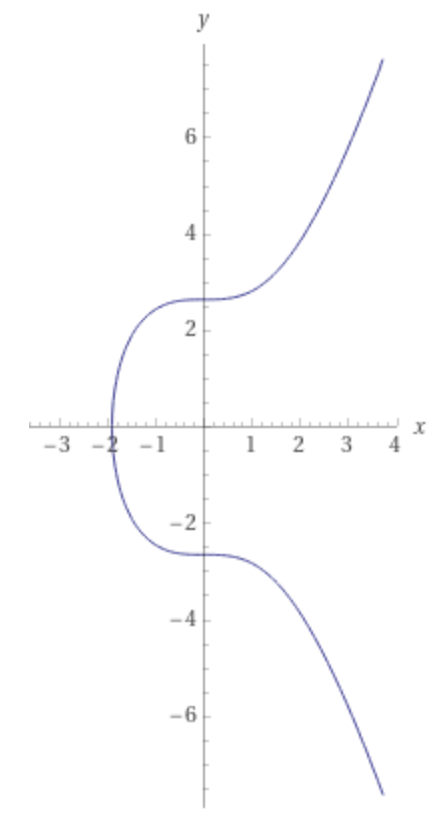
\includegraphics[width=.4\linewidth]{Pictures/bitcoinec.png}
  \caption{\(y^2 = x^3 +7\)}
  \label{fig:test1}
\end{minipage}%
\begin{minipage}{.5\textwidth}
  \centering
  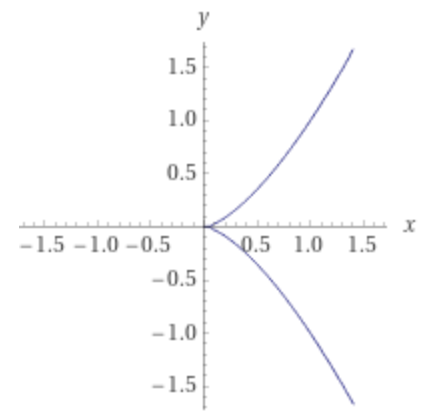
\includegraphics[width=.7\linewidth]{Pictures/y2x3.png}
  \caption{\(y^2 = x^3\)}
  \label{fig:test2}
\end{minipage}
\end{figure}

Elliptic curves are useful for \acrshort{zksnark}s because of the discrete logarithm problem, which is believed to be very hard to solve. Given a point \(g\) on the elliptic curve and a multiple of that point, \(n*g\), it is impossible to solve n, even if \(g\) and \(n*g\) are given. In order to choose an elliptic curve that offers homomorphic hiding, we need to implement a mapping between our known numbers of the finite field \begin{math}\mathbb{F}_p\end{math} and a set of points on the elliptic curve (hidden space). Let \begin{math}\mathbb{F}_p\end{math} be a finite field of order \(p\), whereby \(p\) is a large prime, e.g., if \(p=97\), then \begin{math}\mathbb{F}_p\end{math} \(=\{0, 1, 2, 3, ..., 96\}\) For this, we are going to take a generator point \(g = (x1,y1)\) that lies on the elliptic curve and multiply it with every element \({element}_i\) in \begin{math}\mathbb{F}_p\end{math}. For example, \(g + g = 2*g\) is calculated by putting a tangent line on \(g\), and wherever the line crosses the elliptic curve, we receive the result by using the opposite signs of that point. To arrive at \(2*g + g = 3*g\), the point \(2*g\) is used to draw a line to \(g\), see where the line further intersects with the elliptic curve, and use the opposite signs of that point to arrive at \(3*g\). This is repeated for every \(element\) in \begin{math}\mathbb{F}_p\end{math}. As a result, we have our finite field mapped to a hidden space on the elliptic curve. In summary, every 
\(element\) is hidden by
\begin{align}
    hh(element) = element * g
\end{align}
Additionally, we have to define what 0 and 1 are. The element 0 results from subtracting a point on the elliptic curve, i.e., when point \(g\) goes to infinite. 1 is the point \(g\) itself.
Now, we have achieved homomorphic addition:
\begin{align}
    (A + B) \longrightarrow (A + B) * g = A*g + B*g
\end{align}

In order to use elliptic curve pairing to verify \acrshort{zksnark}s proofs, e.g., Groth16, we need to achieve a limited homomorphic multiplication operator. The hidden space is a group of points generated by the finite field elements and the generation point, \(g1\), on the elliptic curve. Now, we want to choose a subgroup \begin{math} \mathbb{G}_1\end{math} from that group. We choose that subgroup so that the number of elements we chose, \(r\), is a prime number too. Having found \(r\), we can continue to choose the embedding degree of the elliptic curve. In Groth16, the proving key and verification key consist of \begin{math} \mathbb{G}_1\end{math} and \begin{math} \mathbb{G}_2\end{math} element. The embedding degree \(k\) has to be found so that \(p^k-1\ |\ r\), i.e., is a multiple of it. Let us use a minimal example to show how to arrive at \begin{math} \mathbb{G}_1\end{math} and \begin{math} \mathbb{G}_2\end{math}.
Let us define an example base field \begin{math}\mathbb{F}_p\end{math} \(= \{0,1,2\}\) with \(p = 3\). We have found an embedding degree \(k=2\). In order to achieve our goal of creating a subgroup \begin{math} \mathbb{G}_2\end{math}, we need to extend our base field by a defining polynomial. This polynomial is of degree \(k\), and no element of our base field evaluates it to 0. In summary, we have the following:

\begin{align}
    \mathbb{F}_p = \{0,1,2\}, p = 3, k = 2
\end{align}

Defining polynomial for field extension \begin{math}\mathbb{F}_p^k\end{math}: 
\begin{align*}
    f(x) = z^2 +1 \\
    f(0) = 1\\
    f(1) = 2\\
    f(2) = 5 mod 3 = 2
\end{align*}

As shown in (5.18), none of the base field elements make f(x) evaluate to 0. In order to create the elements of the field extension \begin{math}\mathbb{F}_p^k\end{math}, we have to create all possible degree 2 polynomials out of the combinations of our base field \begin{math}\mathbb{F}_p\end{math}. For example, one possible polynomial with the coefficients from our base field is:

\begin{align}
    1*z^2+2*z+0 
\end{align}   
\begin{align*}
    (z^2+2*z)\mod (z^2+1) = 2*z-1\mod 3 = 2*z+2
\end{align*}
\(2*z+2\) is one element of the extension field \begin{math}\mathbb{F}_p^k\end{math}. In total, \begin{math}\mathbb{F}_p^k\end{math} has 9 elements, all calculated as in (5.18). In Summary, the elements of our extension field \begin{math}\mathbb{F}_p^k\end{math} are
\begin{align}
\{0, 1, 2, z, z+1, z+2, 2z, 2z+1, 2z+2\}
\end{align}

As shown in (5.20), the elements of the extension field are polynomials of degree up to \(k-1\). Addition and multiplication are defined in the way that coefficients are calculated \(\mod 3\) and polynomials \(\mod z^2+1\), the defining polynomial  
\(f(x)\) from (5.18).

Now, having our extension field, we can use it to create \begin{math}\mathbb{G}_2\end{math}, a subgroup of points of the same elliptic curve used for \begin{math}\mathbb{G}_1\end{math}, but with elements of \begin{math}\mathbb{F}_p^k\end{math}, instead of base field \begin{math}\mathbb{F}_p\end{math}. For this, we have to define points, whereby x and y coordinates are polynomials from \begin{math}\mathbb{F}_p^k\end{math}. \begin{math}\mathbb{G}_2\end{math} will consist of combinations from \begin{math}\mathbb{F}_p^k\end{math} in the form of \((x,y)\), which satisfy the elliptic curve. 

Pairings are bilinear maps that combine elements of two spaces to receive an element of a third space, e.g., matrix multiplication. In Groth16, the following pairing notation is used:

\begin{align}
    e: \mathbb{G}_1 \times \mathbb{G}_2 \to \mathbb{G}_T
\end{align}

The result of all steps performed previously is an incomplete homomorphic multiplication that enables us to check that the correct polynomial coefficients were used for \(A(x), B(X), \text{ and }C(x)\), as well as the same solution vector \(s\). It is incomplete because not more than two elements can be multiplied. However, this satisfies the use case for \acrshort{zksnark}s. 

\subsubsection{Groth16}

Preliminaries to understand the Groth16 protocol have been covered. In the following, we will describe the setup, proof, and verification steps in Groth16. The parameters are summarized in Table \ref{tab:Groth16Params}.

\setlength{\tabcolsep}{2ex}
\renewcommand{\arraystretch}{1.5}%
\begin{table}[hbt]
	\centering
	    \caption{Groth16 - Parameter Summary}
		\begin{tabular}{| m{0.3\linewidth} | m{0.6\linewidth} |}
		\hline
		\textbf{Parameter} & \textbf{Definition}\\ \hline
            \(n,m\) & number of constraints, number of variables\\ \hline
            \begin{math}\mathbb{F}_p\end{math} & finite field of prime order p\\ \hline 
            \begin{math}\mathbb{G}_1, \mathbb{G}_2, \mathbb{G}_T\end{math} & groups of points of prime order p satisfying an elliptic curve\\ \hline
            \begin{math}\mathbb{G}_1 \times \mathbb{G}_2 \to \mathbb{G}_T\end{math}& bilinear pairing \\ \hline
            \begin{math}g_T = e(g_1, g_2)\end{math}& generators with mapping \\\hline
            \begin{math}\bigl\{A_i(X), B_i(X), C_i(X)\bigl\}_{i=0}^m\end{math} & encoded computation as result of \acrshort{r1cs} and \acrshort{qap}: three sets of polynomials of degree \(n-1\)\\ \hline
            \(Z(x) = (x-1)*(x-2) * \newline (x-3)...(x-(n-1))\) &  minimal polynomial, known because n is known \\ \hline
            \(l\) & number of public inputs \\ \hline
            \((s_1,...,s_l)\) & elements of witness whose inputs are public \newline (e.g., out = 35 in our example) \\ \hline
            \((s_{l+1},s_{l+2},...s_m)\) & elements of witness for secret input x, with \(s_0 = 1\) \\ \hline
	\end{tabular}
\label{tab:Groth16Params}
\end{table}

\subsubsection{Key generation}

The proving and verification keys are obtained from the Common Reference String (\acrshort{crs}) via multi-party computation. From \begin{math}\mathbb{F}_p\end{math}, a set of random values is generated. This toxic waste (tw), or trapdoor, must be secret and forgotten from memory because knowledge of it enables forged proofs. Note that \begin{math}\tau\end{math} is the random point \(P\) from our examples. From the toxic waste, polynomial \(L_i(x)\) is defined:
\begin{align}
    tw = (\alpha, \beta, \gamma, \delta, \tau) 
\end{align}
\begin{align*}
    L_i(x) = \beta * A_i(X) + \alpha * B_i(X) + C_i(X)
\end{align*}
The \acrshort{crs} consist of \begin{math} \sigma = ([\sigma_1]_1,[\sigma_2]_2)\end{math}, which are elements of \begin{math} \mathbb{G}_1, \mathbb{G}_2\end{math}.

\begin{align}
    [\sigma_1]_1 = 
    &\ [(\alpha, \beta, \gamma, \delta, \\
    &\ 1, \tau, \tau^2, \tau^3, ..., \tau^{n-1}, \\
    &\ \frac{L_0(\tau)}{\gamma}, ..., \frac{L_l(\tau)}{\gamma}, \\
    &\ \frac{L_{l+1}(\tau)}{\delta}, ..., \frac{L_m(\tau)}{\delta})]_1 
\end{align}
\begin{align*}
    [\sigma_2]_2 = [(\beta, \gamma, \delta, \ 1, \tau, \tau^2, \tau^3, ..., \tau^{n-1})]_2
\end{align*}

\begin{itemize}
    \item (5.23): elements of the toxic waste
    \item (5.24): powers of \begin{math}\tau\end{math} of degree up to \(n-1\)
    \item (5.25): The polynomial is chosen from the set of polynomials of \(A(X), B(X), C(X)\), which corresponds to the place of the public input of the solution vector. In our starting example, \(out = 35\) is the public input (since this is our only public input, \(l=1\)). The public input is in third place in s. Hence, \(A_3(X), B_3(X), C_3(X)\) are chosen, evaluated at \begin{math}\tau\end{math} and multiplied by \begin{math} \alpha, \beta\end{math}.
    \item (5.26): Same as (5.25), but for the non-public inputs of \(s\). All elements of \begin{math} [\sigma_1]_1 \end{math} are \begin{math}\mathbb{G}_1\end{math} elements, e.g., \begin{math}\alpha_1 = g_1 * \alpha\end{math}.
\end{itemize}

The proving key consists of the following elements:
\begin{itemize}
    \item \([(\alpha, \beta, 1, \tau, \tau^2, \tau^3, ..., \tau^{n-1}, \frac{L_{l+1}(\tau)}{\delta}, ..., \frac{L_m(\tau)}{\delta})]_1\)
    \item \([(1, \gamma, \delta)]_2\)
    \item circuit information about the polynomials:
    
    \(A_0(X), A_1(X), ..., A_m(X)\)
    
    \(B_0(X), B_1(X), ..., B_m(X)\)
    
    \(C_0(X), C_1(X), ..., C_m(X)\)
    
    \(Z(x) = (x-1)(x-2)(x-3)...(x-(n-1))\)
\end{itemize}

The verification key consists of the following elements:
\begin{itemize}
    \item \([(1, \frac{L_0(\tau)}{\gamma}, ..., \frac{L_l(\tau)}{\gamma})]_1\)
    \item \([(1, \gamma, \delta)]_2\)
    \item precomputed pairing \([\alpha * \beta]_T\), which is a \begin{math}\mathbb{G}_T\end{math} element
\end{itemize}

\subsubsection{Generating the proof}

Two random numbers \(r, t\) are generated from \begin{math}\mathbb{F}_p\end{math}, that are used to compute

\begin{enumerate}
    \item \begin{math} A= \alpha + s_0*A_0(\tau) + s_1*A_1(\tau) + ... + s_m*A_m(\tau) + r\delta\end{math}
    \item \begin{math} B= \beta + s_0*B_0(\tau) + s_1*B_1(\tau) + ... + s_m*B_m(\tau) + t\delta\end{math}
    \item \begin{math} C= \frac{s_{l+1}L_{l+1}(\tau)}{\delta} + \frac{s_{l+2}L_{l+2}(\tau)} + ... +\frac{s_{lm}L_{lm}(\tau)}{\delta} + \frac{H(\tau)Z(\tau)}{\delta} + At + Br - rt\delta\end{math}
\end{enumerate}

The proof \begin{math}\pi\end{math} consists of two elements from \begin{math}\mathbb{G}_1\end{math} and one element from \begin{math}\mathbb{G}_2\end{math}:
\begin{align}
    \pi = ([A]_1, [B]_2, [C]_1)
\end{align}

\subsubsection{Verification}

In Groth16, three pairings are checked during verification. \begin{math}[\alpha * \beta]_T\end{math} is a precomputed pairing and is made available in the setup phase. The verification computation receives proof \begin{math} \pi\end{math} and accepts it only if the following equation holds:
\begin{align}
    [A]_1 * [B]_2 = [\alpha]_1[\beta]_2 + \bigl[\frac{s_0L_0(\tau)}{\gamma}+ \frac{s_1L_1(\tau)}{\gamma} + ... + \frac{s_lL_l(\tau)}{\gamma}\bigr]_1 * [\gamma]_2 + [C]_1 * [\delta]_2
\end{align}

As shown in (5.28), the following three pairings are needed to be checked:

\begin{itemize}
    \item \(e([A]_1, [B]_2)\)
    \item \begin{math}
        e(\bigl[\frac{s_0L_0(\tau)}{\gamma}+ \frac{s_1L_1(\tau)}{\gamma} + ... + \frac{s_lL_l(\tau)}{\gamma}\bigr]_1 , [\gamma]_2)
    \end{math}
    \item \begin{math}
        e([C]_1, [\delta]_2)
    \end{math}
\end{itemize}

Let us evaluate the verification equation in (5.28). The left-hand side evaluates as follows:

\begin{equation*}
\begin{split}
    [A]_1 * [B]_2 = [A*B]_T &= [\alpha + s_0*A_0(\tau) + s_1*A_1(\tau) + ... + s_m*A_m(\tau) + r\delta]_1 \ *\\
    &\ \ \ \ [\beta + s_0*B_0(\tau) + s_1*B_1(\tau) + ... + s_m*B_m(\tau) + t\delta]_2 \\
    &= [(\alpha + A(\tau) + r\delta) * (\beta + B(\tau) + t\delta)]_T\\
    &= [\alpha * \beta]_T + [\alpha * B(\tau)]_T + [\alpha * t\delta]_T \ + [A(\tau) * \beta]_T \ + \\
    &\ \ \ \ [A(\tau) * B(\tau)]_T + [A(\tau) * t\delta]_T + [r\delta * \beta]_T + [r\delta * B(\tau)]_T +\\
    &\ \ \ \ [r\delta * t\delta]_T \\
    \\
    &= [A(\tau) * B(\tau)]_T \textcolor{orange}{\ +\ [\alpha * \beta]_T + [\alpha * B(\tau)]_T + [\alpha * t\delta]_T} \\
    &\ \ \textcolor{orange}{+ [A(\tau) * \beta]_T \ + [A(\tau) * t\delta]_T + [r\delta * \beta]_T + [r\delta * B(\tau)]_T} \\
    &\ \ \textcolor{orange}{+ [r\delta * t\delta]_T}
\end{split}
\end{equation*}

The right-hand side evaluates to:
 \begin{equation*}
     \begin{split}
    &=[\alpha]_1[\beta]_2 + \bigl[\frac{s_0L_0(\tau)}{\gamma}+ \frac{s_1L_1(\tau)}{\gamma} + ... + \frac{s_lL_l(\tau)}{\gamma}\bigr]_1 * [\gamma]_2 + [C]_1 * [\delta]_2 \\
    &=[\alpha * \beta]_T + [(s_0L_0(\tau) + s_1L_1(\tau) + ... + s_lL_l(\tau))]_T + [(s_{l+1}L_{l+1}(\tau) + s_{l+2}L_{l+2}(\tau) + ... \\
    &\ \ \ + s_{lm}L_{lm}(\tau)) + H(\tau)Z(\tau) + At\delta + Br\delta - rt\delta\delta]_T
     \end{split}
 \end{equation*}

Now, we can replace A and B. We also see that the middle of the equation is \(L_i(\tau)\).
 \begin{equation*}
     \begin{split}
     &=[H(\tau) * Z(\tau) + C(\tau)]_T \textcolor{orange}{\ +\  [\alpha * \beta]_T + [\alpha * B(\tau)]_T + [\alpha * t\delta]_T + [A(\tau) * \beta]_T} \\
     &\ \ \ \textcolor{orange}{+ [A(\tau) * t\delta]_T + [r\delta * \beta]_T + [r\delta * B(\tau)]_T + [r\delta * t\delta]_T}
     \end{split}
 \end{equation*}

Eventually, we got the equality check we wanted to achieve (5.15). The use of the secret encoded values \(\alpha, \beta\) of the toxic waste (5.22) forces the prover algorithm to use the same coefficients of the solution vector (witness) to compute \(A(X), B(X), C(X)\). \(\gamma, \delta\) ensure that the public inputs of order \(l\) are independent from the solution vector (witness). In order to achieve the zero-knowledge aspect, \(r, s\) are used to shift the proof randomly.

\section{PLONK-based zk-DApp}
The decentralized application for zero-knowledge \acrshort{mro} data attestation (\acrshort{zkdapp}) facilitates data entries and data sharing between \acrshort{mro} data owners (submitters) and aviation authorities (attesters) in zero-knowledge. This software artifact attempts to ensure compatibility between the lack of trust among industry participants and the need for data verification and transparency (a trade-off between requirements within the project). \acrshort{mro} data need to be transparent for potential secondary market trading of aviation spare parts without giving full access to the documentation, e.g., to the entire shop report.

\subsection{Implementation}
The zero-knowledge part of the \acrshort{zkdapp} is implemented via circom and snarkjs, developed by iden3. iden3 is an open-source project focused on scalable and distributed identity systems on zero-knowledge proofs, i.e., providing protocols, data structures, and modules. The current objectives include achieving self-sovereign identities free of charge, minimizing on-chain transactions, re-designing privacy with non-reusable proofs, creating complete products, e.g., user wallets, and focusing on community standardization \citep{iden3aboutus}. Circom is Rust-based and allows one to write and compile arithmetic circuits. In circom, there is a data type called field elements, which per default represents values modulo a large prime number based on the BN128 elliptic curve \citep{circom}. \acrshort{r1cs} files are generated by compiling the circuit: the constraint system in binary format, a symbols file for debugging, and files that are necessary to generate the witness. In order to compute the witness, an input file in JSON format needs to be specified that contains the witness information. 

In the \acrshort{zkdapp}, the submitter enters the information to be verified, which is processed according to an input schema. The witness is computed and saved in a file format accepted by snarkjs. Snarkjs is a JavaScript library that continues with the outputs from circom and executes a specified zero-knowledge proof protocol, e.g., currently, Groth16, \acrshort{plonk}, and Fflonk are supported \citep{snarkjsdoc}. For this use case, snarkjs' \acrshort{plonk} implementation is utilized. For the verification and intermediate result hashes, a powers of tau file is utilized to perform the multi-party computation. In Groth16, it is utilized during the trusted setup (5.2.1). In \acrshort{plonk}, this is the source of public randomness (5.2.2). Figure \ref{fig:zk-DAppgeneral} shows the main steps performed for a \acrshort{plonk}-based \acrshort{zkdapp}. \acrshort{plonk} does not require a trusted ceremony for each circuit, i.e., the powers of tau ceremony is universal. After compiling the circuit and calculating the witness, the snarkjs \acrshort{plonk} can be set up. A final protocol transcript key (zkey) is generated and verified. The zero-knowledge key includes proving and verification key \citep{snarkjsdoc}. From the zkey, the verification key is exported in JSON format. With this verification key file, the final zkey file and the witness file, the proof file, and the file with the public inputs and outputs are generated. These two files and the verification key are used to verify the proof. The verifier is transformed into a smart contract (PlonkVerifier.sol) that performs the verification. In order to utilize the PlonkVerifier smart contract exported in the previous step, an interface must be created (IPlonkVerifier.sol), which initiates verifyProof and outputs a true or false. The ZkDocument.sol smart contract, which stores user inputs, e.g., the commitments and trusted attesters, uses this interface to verify the proof and update the states of the smart contracts. With every user input, a witness and proof are calculated. The commitment is posted, and the smart contracts are updated. Once verified, the user interface (UI) shows an update, e.g., a green highlighting. 
\begin{figure}[hbt]
	\centering
		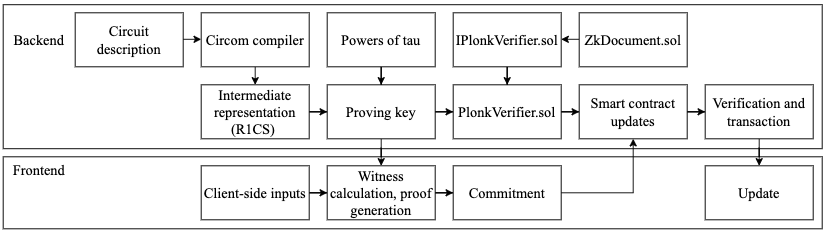
\includegraphics[width=1.0\textwidth]{Pictures/circom snarkjs process flow.png}
	\caption{\acrshort{plonk}-based \acrshort{zkdapp} Interaction Process Flow}
	\label{fig:zk-DAppgeneral}
\end{figure}
For deployment, broadcasting, and development, hardhat testnet is used. Metamask is used as a crypto wallet browser plugin.

\subsection{Artifact}
Different roles and the steps to be performed in the \acrshort{zkdapp} are described as follows.
\begin{enumerate}
\item The process flow and general functionalities are depicted.
\item Essential implementation logic and features are highlighted with references to the implementation code.
\end{enumerate}
For the \acrshort{zkdapp} to start, the command \textit{yarn start} needs to be executed in the zkdocs-backend directory. It will start the hardhat test network and show a set of test accounts with private keys to use. These test accounts are also used for the accounts of the verifier, submitter, and attesters. The following command in Figure \ref{fig:second-cmd} is also run in the same directory and deploys the schema for the \acrshort{mro} data entry. It triggers the circom and snarkjs ceremonies and shows the number of constraints, inputs, outputs, wires, and labels in the arithmetic circuit. Also, it shows that the corresponding \acrshort{r1cs}, symbols, and witness-generating files are written successfully. Once the setup is finished, the public keys of the deployer (submitter), \acrshort{plonk} verifier (PlonkVerifier.sol smart contract address), and zkDoc (ZkDocument.sol smart contract address) are shown. The zkDoc public key needs to be parsed every time another set of inputs needs to be made or verification needs to be performed. Ultimately, the schema is created, and the corresponding directories are listed. The UI can be started with the same command \textit{yarn start} in the zkdocs-ui directory.

\begin{figure}[hbt]
	\centering
		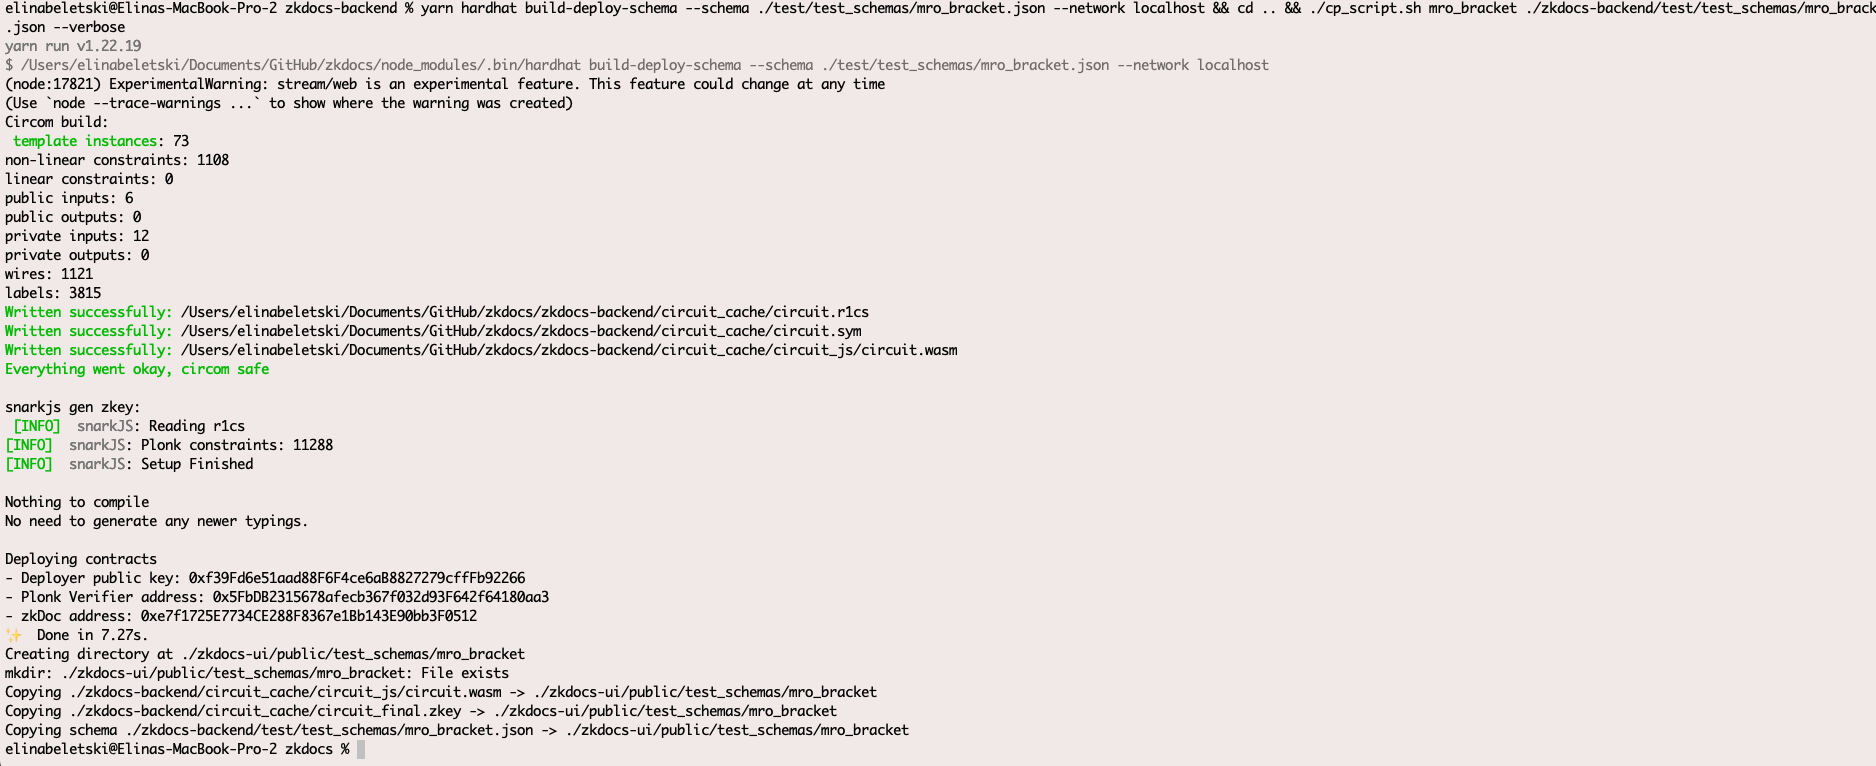
\includegraphics[width=1.0\textwidth]{Pictures/second-cmd.png}
	\caption{Initiating the Deployment of \acrshort{plonk} in circom, snarkjs in the \acrshort{zkdapp} Backend}
	\label{fig:second-cmd}
\end{figure}

\subsubsection{Sequence of events}
The \acrshort{zkdapp} has three roles: verifier, submitter, and attester. In this scenario, the verifier also acts as administrator, operating the \acrshort{zkdapp}. Hence, the administrator operates the schema with constraints, fields, and the list of trusted institutions that can attest in the \acrshort{zkdapp}. The submitter owns \acrshort{mro} data and seeks validation. The attester is assigned to view specific information shared with them and can validate it, i.e., attest to the data provided. The verifier can obtain the proof and verify it. Other stakeholders in the system can learn that there is verified information but do not learn anything besides its correctness. The following sequence of events refers to the landing page of the \acrshort{zkdapp} (Figure \ref{fig:landing-page}).
\begin{figure}[hbt]
	\centering
		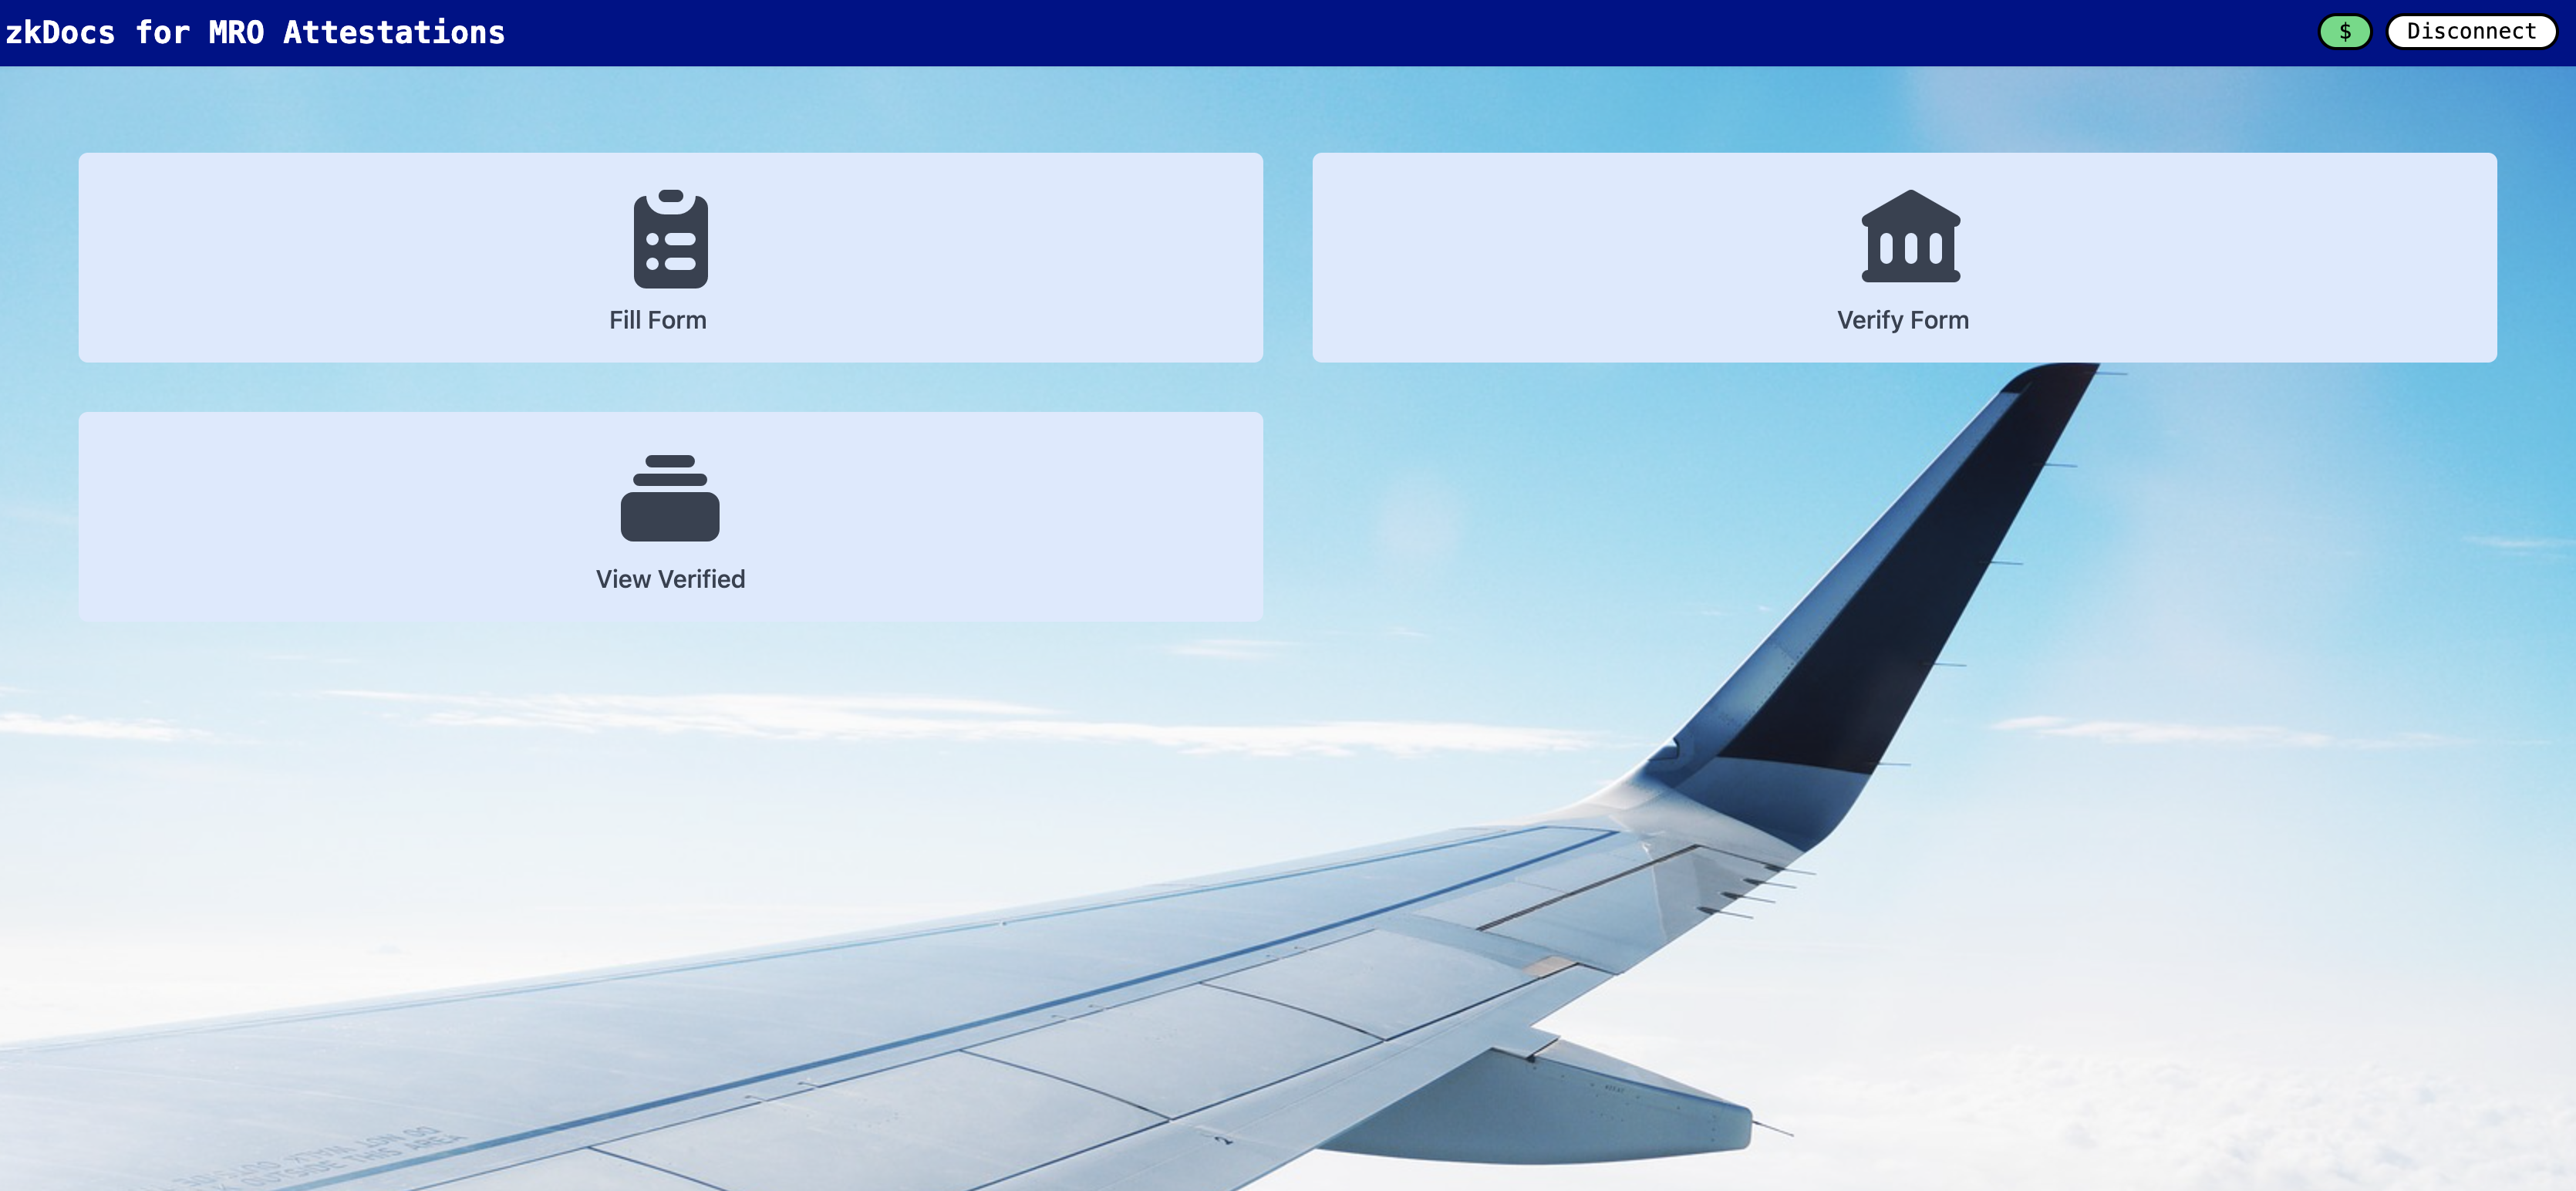
\includegraphics[width=1.0\textwidth]{Pictures/landingpage.png}
	\caption{\acrshort{zkdapp} Landing Page}
	\label{fig:landing-page}
\end{figure}
\begin{enumerate}
\item \textit{Fill Form}:
The submitter connects their wallet and can see an input mask for \acrshort{mro} data entries (Figure \ref{fig:form}. In this prototype, the submitter can enter the part identifier, flight hours, time since the last service, and \acrshort{mro} cycles. Once the values are added, the submitter decides which authority needs to attest to the values, e.g., \acrshort{faa}, \acrshort{easa}. If the constraints are met, the submitter generates the proof, which results in the following: First, the proof is generated and displayed. Second, communication links are generated, which can be parsed in another browser tab. These links are specific to the respective attesters, so the data assigned to them can be viewed. In practice, this has to be realized via separate communication channels to alert attesters once a new set of \acrshort{mro} data inputs is performed. The submitter commits to these entries and the proof on-chain. Now, the values can be viewed by the respective attester and validated.

\item \textit{Attest to \acrshort{mro} data}: The respective attester follows the attestation link, connects their wallet, and only sees the decrypted values of the data assigned to them for validation. The attester marks the data as valid and commits the result. Verification can be initiated once all attesters have successfully attested to the data.

\item \textit{Verify Form}: Another user, e.g., the administrator, the submitter, or any dedicated user with the proof, can perform the verification. The verifier connects their wallet and checks the attestations. The only information available is the green mark, that data has been successfully attested to, which fields have been attested to, and who attested to these fields and values. The values are shown in an encrypted format. With the proof parsed, the verifier can verify and submit. If the attestations are correct, a bit will be flipped in the smart contract \citep{zkdocs}, and the verification will be successfully performed.

\item \textit{View Verified}: Any participant can view the latest verified information. However, only the green mark shows whether the data is correct, the field names, and which trusted authority performed the attestation. The verifier and other participants learn nothing besides that the information provided is correct and has been truthfully attested by a trusted institution.
\end{enumerate}

\begin{figure}[hbt]
	\centering
		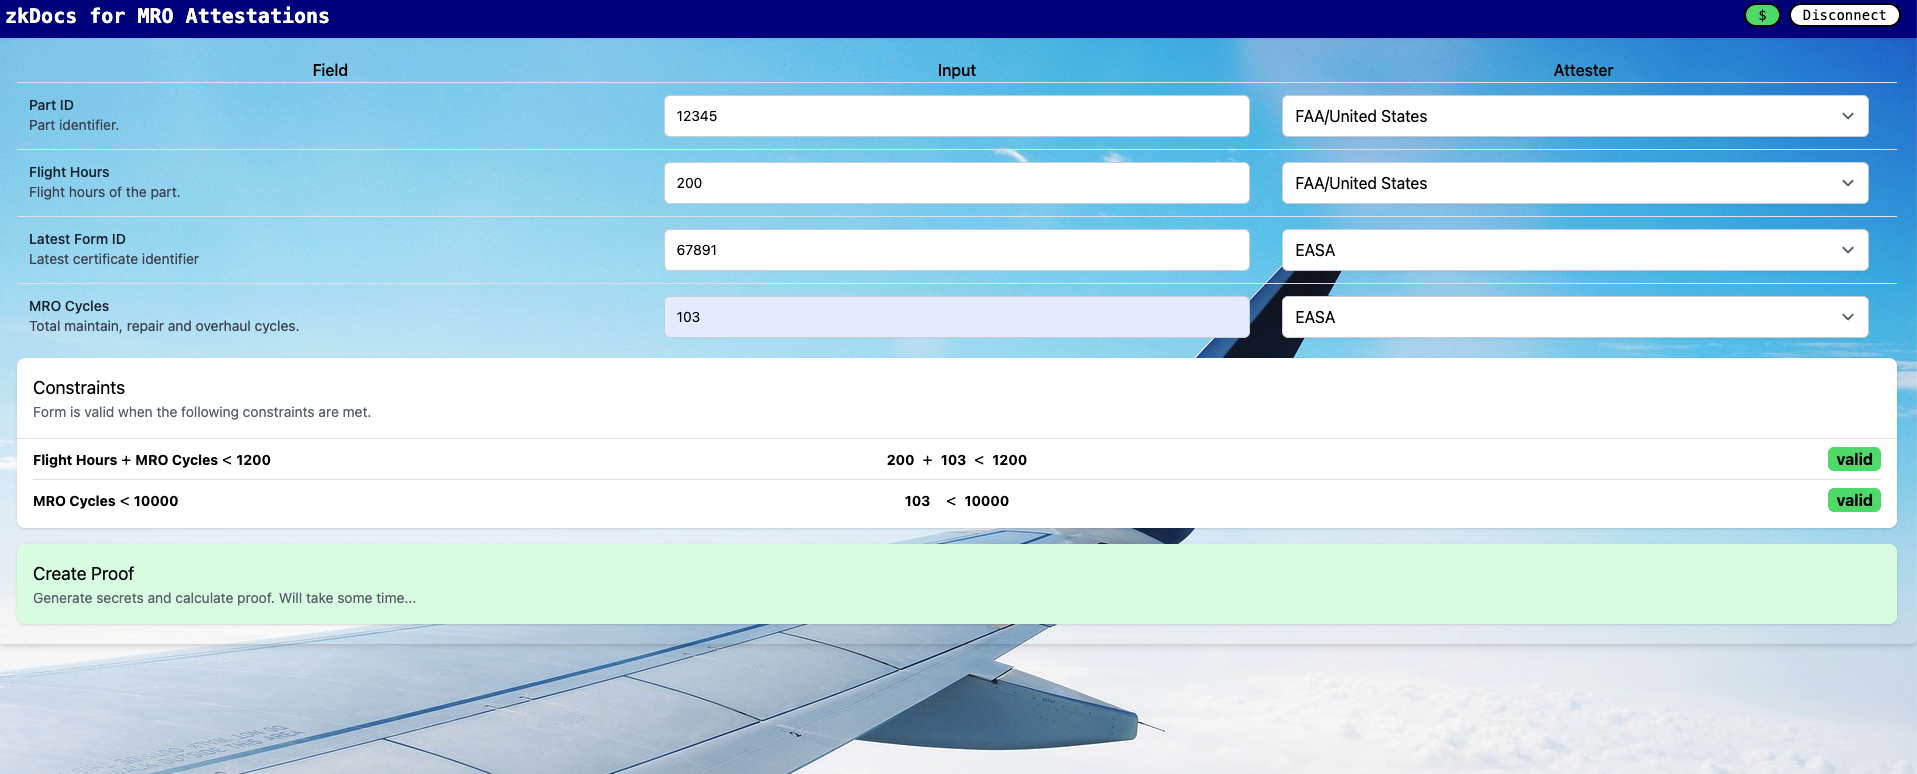
\includegraphics[width=1.0\textwidth]{Pictures/form.png}
	\caption{\acrshort{zkdapp} Fill Form (Initial)}
	\label{fig:form}
\end{figure}

\subsubsection{Highlighted features}
The following features illustrate the underlying functionality applied in the \acrshort{zkdapp}.


The circuit and witness calculation input is processed through a schema. The JSON template is a rule book for the input field and values, constraints, and trusted attesting addresses. \textit{ZkDocSchema.ts} uses the JSON template to define the schema. It sets valid operators and constraint types and validates if the template matches those. Some further value validations are build-in as well, e.g., checks for non-negative numbers. 

\textit{ZkDocGenerator.ts} acts as wrapper for circom and snarkjs. It contains all necessary commands to initiate the circuit, represent intermediate formats, e.g., \acrshort{r1cs}, calculate the witness and the zero-knowledge key file, and export the verifier as smart contract. It generates the constraint string and looks up the field indices of the fields to attest in the schema. The circuit's functionality is specified in \textit{circuit.circom}. It defines the constraints checks for each field if the commitment matches the hashed commitment on-chain. During attestation, the assigned attester performs the decryption of the values locally.

The actual user input values are handled in the \textit{ZkDocument.sol} smart contract. It stores the selected attester addresses, the submitter's address, field commitments, and field indices to be attested. A nonce is generated for each field and value, and the commitment scheme is initiated. The commitment scheme for each field is hash(value, nonce). The hashing algorithm used in the circuit is POSEIDON. Due to its reduced prover and verifier complexity, POSEIDON is currently favored in research and developing zero-knowledge decentralized applications. Unlike other popular hashing functions, e.g., SHA-256, POSEIDON can operate on smaller circuits and is adapted to finite fields \citep{poseidon}. It can add and remove trusted attesters from the list via \textit{(addValidInstitution, addValidInstitutions, removeValidInstitution)}. It ensures that only the attester specified by the submitter via mask entry can attest to the fields and values committed. During this check, it is also secured that the attestation's field index matches the one specified during submission. Once the check is successful, the bit is flipped to confirm the correctness of the attestation. This procedure is simultaneously applied to all field attestations via \textit{attestMultiple}. 

The function \textit{postFields} posts the commitments and checks that 1. the commitment length matches the number of fields, 2. the correct number of institutions to perform attestations are in the commitment, and 3. the commitment is unique, and has not been posted previously. Through \textit{validateSubmitter}, the public signal array for \acrshort{plonk} verification is filled with the commitments. It checks that the specified institutions have attested to all fields. As described in the introduction of circom and snarkjs in Chapter 6.2, the verifier is transformed to a Solidity smart contract \textit{PlonkVerifier.sol}), containing the values and function logic needed for \acrshort{plonk} verification. \textit{ZkDocument.sol} uses the interface to \textit{PlonkVerifier.sol}, the \textit{IPlonkVerifier.sol} to initiate the function \textit{verifyProof}, which verifies the proof. By using the interface, it is made sure that a specific standardized function from the generated \textit{PlonkVerifier.sol} is used (\textit{verifyProof}). This way of implementation ensures that the state of \textit{PlonkVerifier.sol} undergoes an actual change. In order to prevent client-side attacks, the schema hash, using the Keccak-256 hashing algorithm (part of SHA-3 Solidity family), is stored in \textit{ZkDocument.sol} as well. 

The UI finds the correct schema via the scheme hash stored, facilitated through \textit{SchemaUtils.ts}. It obtains the corresponding schema from the schema hash and can utilize the files generated through the \acrshort{plonk} procedure in circom and snarkjs. Additional Figures are provided in Appendix \ref{Appendix B}.
\begin{comment}
ÜBERLEITUNG: 
- use case support system for predictive maintenance
- \acrshort{mro} KPIs are found in different documents, have to be attested by different institutions: e.g. shop report -->repair shop, release certificate-->aviation authority
- also for trading this is important information 
- this use case resulted from requirement privacy and transparency as well as trading of parts
- assumption: data is available
- überleitung zur daten architektur: automatic verification of part id and its true existence through merkle tree zk verification
\end{comment}

\section{Evaluation}

\subsubsection{\acrshort{zkdapp} \acrshort{mro} Attestations}
On the developer's machine with a 2,2 GHz 6-Core Intel Core i7 processor and macOS 13.2.1 (22D68) operating system, the circom build, snarkjs \acrshort{plonk} setup, and contracts deployment is executed in 6.90 seconds. Although it has weaknesses compared to Groth16, the implementation with \acrshort{plonk} is motivated by its capability to be built on top of any polynomial commitment scheme. This feature makes it applicable in zk-Rollups, i.e., the compatibility with the EVM (Ethereum Virtual Machine) is responsible for the massive scaling of the Ethereum blockchain. Additionally, there is the outlook for the future availability of the snarkjs TURBOPLONK, whereby the number of gates is decreased by introducing custom gates appearing multiple times within a circuit. Comparisons with implementations based on the MiMC hash show that \acrshort{plonk} outperforms Groth16 2.5 times \citep{turboplonk}. While the performance depends on the underlying curves and their field sizes, resulting in different pairing friendliness, recent comparisons with Poseidon-128 show less prover time with \acrshort{plonk}. \acrshort{plonk} operates with a larger proof size, i.e., 9 elements in \begin{math} \mathbb{G}\end{math} and additional 7 field elements in \begin{math} \mathbb{F}\end{math} \citep{PLONKcryptoeprint:2019/953}. In comparison, Groth16 only needs 2 elements in \begin{math} \mathbb{G}_1\end{math} and 2 elements in \begin{math} \mathbb{G}_2\end{math}. Any smart contract modification, e.g., circuit change, needs a new trusted setup. For the Aztec protocol, the private transaction protocol for the Ethereum mainnet, this procedure took more than six weeks \citep{turboplonk}. All \acrshort{zksnark} implementations need a trusted setup, which can be made less centralized via \acrshort{mpc}. An \acrshort{mpc} is characterized by many different parties initializing the generation of proving and the verifying key for the trusted setup \citep{Thaler}. 

The result of the evaluation cycle is described as follows, taking feedback from the recent project workshop into consideration: The implementation of the software artifact \acrshort{zkdapp} represents a seized opportunity to meet the second project requirement of constructing a trade-off between privacy, confidentiality, and transparency. This requirement is successfully met due to the nature of zero-knowledge proofs realizing transparency and confidentiality in a trustless environment of \acrshort{mro} spare parts validation. 

On the one hand, the use case of \acrshort{mro} key performance indicator (\acrshort{kpi}) validation needs to be revisited and could be replaced to meet more urgent project targets, e.g., validation of non-\acrshort{kpi} relevant \acrshort{mro} data. The data in the prototype is captured per part identifier only, i.e., the form identifier is obsolete for this prototype. The time since the last service on the part was performed is also relevant and should be added as a third constraint (Figure \ref{fig:form}). The data points are to be perceived as stand-alone, i.e., validation calculation checks and threshold values yet have to be investigated. Except for the data points, further content analysis and feedback in the \acrshort{mro} industry will be performed in future research to match the use case in this prototype in more granularity.

On the other hand, the demonstration of the technical functionality is successful, and the previously developed \acrshort{dapp} for \acrshort{mro} certificate validation and the \acrshort{mro} Smart Hub (in development through Opremic GmbH) can be extended with the zero-knowledge proof functionality of this software artifact. The current code shared with the thesis shows the implementation of the most recent feedback of the evaluation cycle. A screenshot of the input screen (in analogy to Figure \ref{fig:form}) is shown below (Figure \ref{fig:form1}).
\begin{figure}[hbt]
	\centering
		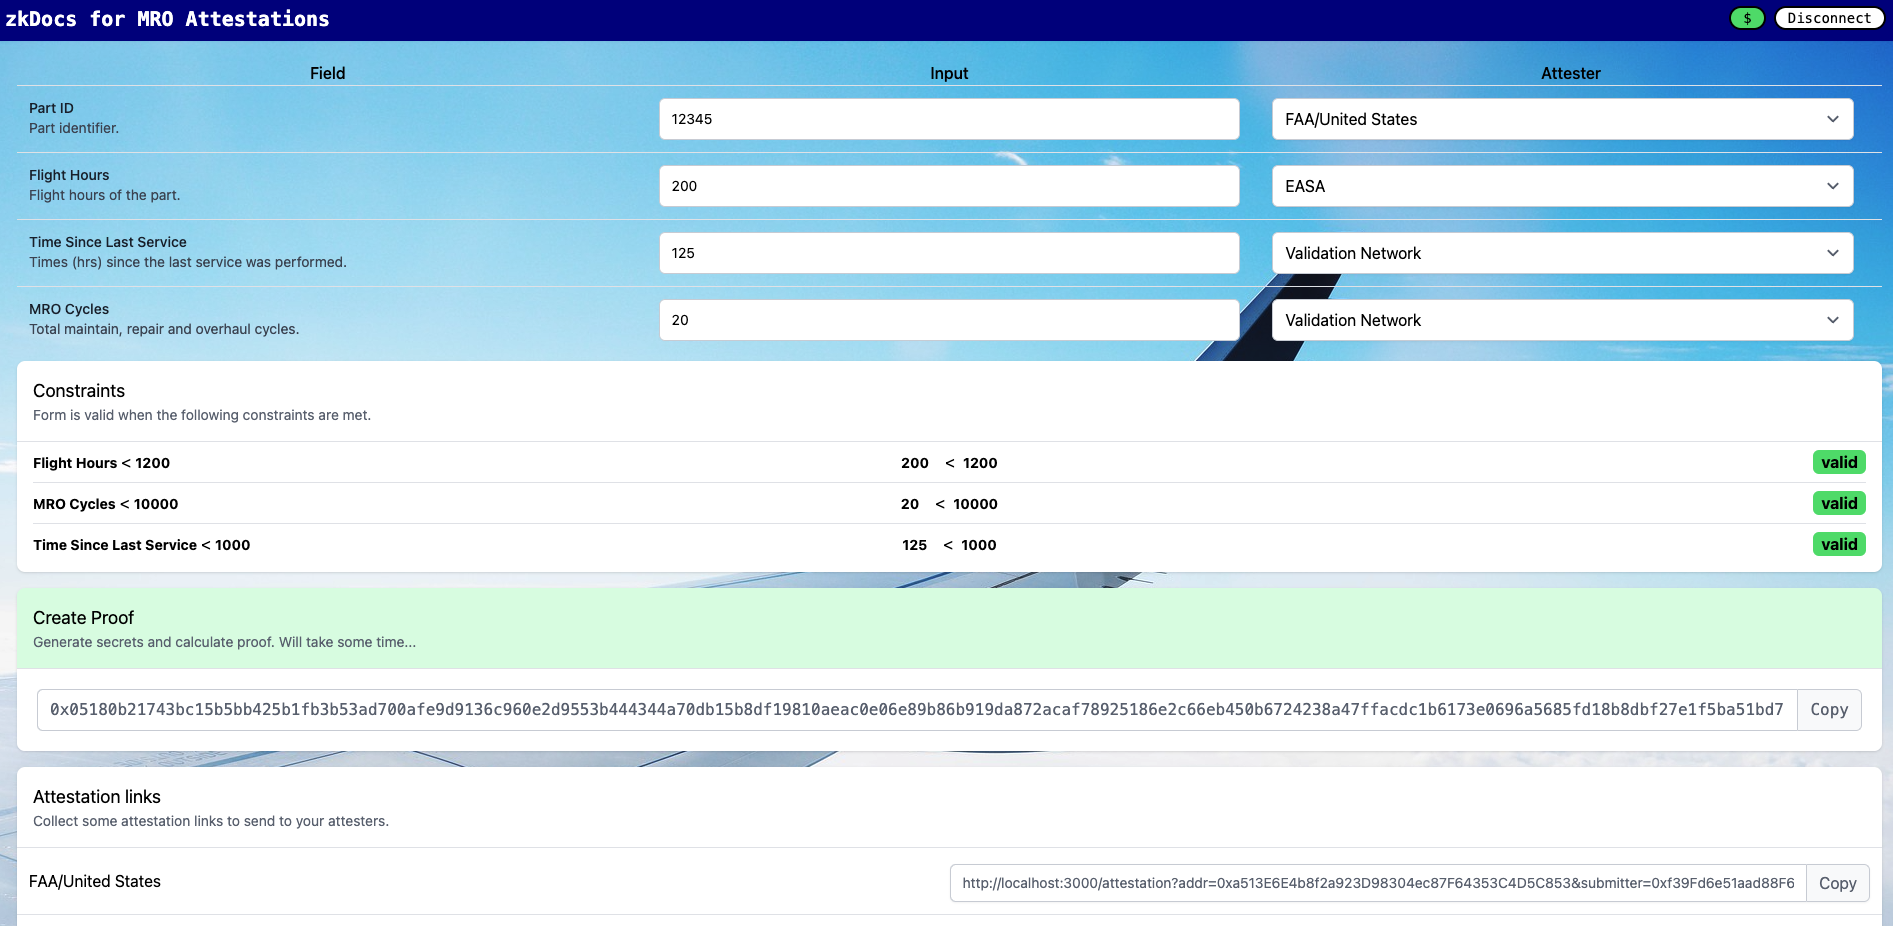
\includegraphics[width=1.0\textwidth]{Pictures/form1.png}
	\caption{\acrshort{zkdapp} Fill Form (Follow-Up after Evaluation)}
	\label{fig:form1}
\end{figure}
Assumptions about the data structure led to the development of the first \acrshort{zkdapp} prototype and are revisited during the evaluation cycle to review the application's data layer in more detail. Current paper-based documentation must be replaced by the automatic digitization of spare part certificates and brought into a practical storage structure with part identifiers and corresponding certificate identifiers. While the automatic digitization of spare part documents is being realized in the project via optical character recognition (OCR), the authenticity validation check of these data in a trustless environment is still to be approached. As an evaluation aspect for further research implementation, an architectural zero-knowledge data structure is outlined as an opportunity to meet the third project requirement. In parallel, this architecture is the basis to increasingly capture \acrshort{mro} \acrshort{kpi} data through combination with the \acrshort{zkdapp} in further research. 

\subsubsection{Zero-Knowledge Data Structure}
The lack of a structured data foundation for proofing the authenticity of aviation spare part documentation is an obstacle to enabling an industry-wide adoption of a blockchain-based industry standard for document verification approaches. In combination with the document issuing organization, there is a need to prove the authenticity of documents, e.g., via a transparent availability of the mechanic's signature and the document date stamp. However, this need for transparency conflicts with data privacy and the large amount of paper-based data captured in the past, which cannot be traced back effectively. Exploring a Merkle-tree-based, zero-knowledge proof data structure satisfies the third requirement to ensure document authenticity and data integrity. Further maturation of this architecture, especially the degree of integration with the \acrshort{zkdapp} prototype, must be addressed further.

Incoming \acrshort{mro} data is structured via a Merkle tree, which is initialized by an aggregator role, the operator. The operator receives data sent by the client, e.g., a \acrshort{zkdapp}. The operator maintains the Merkle tree locally. Once \acrshort{mro} data is submitted, newly created leaves are added to the Merkle tree. The structure is organized as follows: spare parts and subordinated certificates have a unique identifier, e.g., a part identifier has many certificates, each with a unique part id and certificate id combination. Each certificate is issued by an organization that employs mechanics. Mechanics service spare parts, generate \acrshort{mro} data and sign the certificate. The leaves contain the mechanics signature, the \acrshort{mro} data, e.g., the same values collected via the \acrshort{zkdapp} prototype, and a time stamp—the Merkle root results from a specific state of the spare part documentation history. The Merkle tree represents the local running account for \acrshort{mro} data capturing and is entirely maintained off-chain. 

The architecture (Figure \ref{fig:arch}) ensures local and global data integrity. The operator is responsible for proving local data integrity. Through Merkle proofs and blockchain receipts, users can track whether their submitted data was correctly included in the structure. The operator keeps its local Merkle tree with sensitive \acrshort{mro} data off-chain but maintains the Merkle root via blockchain. Users must trust the operator with their data privacy during transfer, but not with the integrity of maintaining correct account keeping \citep{sedlemeirgrenenergy}. 

\begin{figure}[hbt]
	\centering
		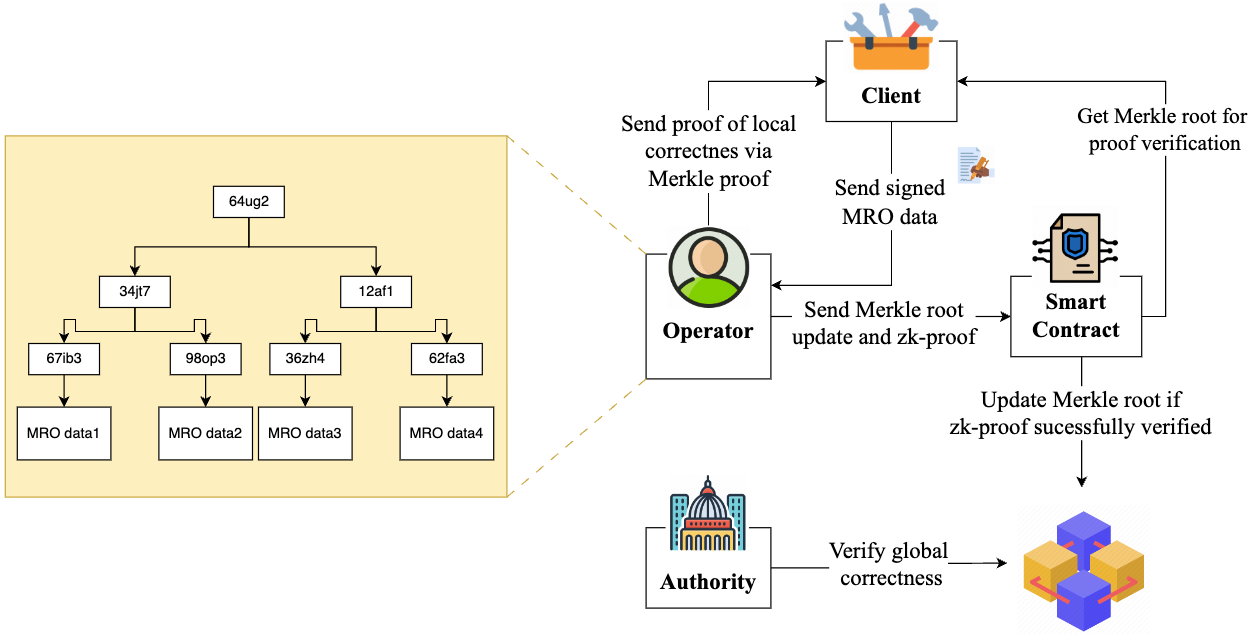
\includegraphics[width=1.0\textwidth]{Pictures/architecture.png}
	\caption{Zero-Knowledge Data Structure Architecture}
	\label{fig:arch}
\end{figure}
Data integrity is not achieved through trust due to this architecture's introduction of zero-knowledge proofs. In order to decentralize the accounting for correct \acrshort{mro} data submission and to prevent fraud on the side of the operator, the use of Merkle proofs alone is not yet sufficient. It needs to be ensured that the generation of \acrshort{mro} data matches globally in the Merkle tree structure. In order to prove the authenticity of any newly batched update, the operator sends the suggestion for the new Merkle root to a smart contract as zero-knowledge proof during periodical Merkle tree updates. As it is known with \acrshort{zksnark}s, all parties must agree on a proving and a verifying key via \acrshort{mpc}, i.e., the trusted setup is initialized. Public inputs are previously correct Merkle root updates. The witness is the signed input submitted by the users and the entire Merkle tree. With this at hand, the operator can generate a zero-knowledge proof to be sent to the smart contract. The smart contract can then verify this proof through the verifying key and the previous Merkle root. Once the proof is considered valid through most nodes participating, the Merkle root can be updated in the smart contract, creating global integrity and transparency for third-party audits. 

This proposal for a zero-knowledge data structure provides the scope to securely manage the documentation of spare parts and certificate data and prove their authenticity by incorporating a zk-rollup-based architecture.


\begin{comment}
- USE CASE: check the authenticity of MRO spare part documentation-->currently hard to achieve due to paper based documentation
- big need to prove authenticity, e.g., through checking if mechanic and date stempel match with a part if and certificate id
- big need to strive towards a decentralized temper-proof data structure
-create a architecture for verification mechanisms in Rapado, based on Sedlmeier, Völter, Strüker (2021):
-->proof membership in a merkle tree? data structure of parts, certificates

- Campanelli et al 2022: improvement on zkSNARKS with Merkle Trees -->HARISA, could be used for the architecture

- build zk DAPP for document verification with circom snarkjs on hardhat test network
- maybe use snarkjs Groth16 first and then Plonk as future outlook, when TurboPlonk support will come in snarkjs

-do one evaluation cycle: which design requirements are met?

feedback from Opremic: 
- MRO data tracked per part Id
- add time since last service as entry, remove form id
- add third constraint
- constraints are stand-alone, no equations yet identified
-add generic attester: Validation Network
- more systematic user interviews needed for this use case, but technical functionality is easily displayed via this use case

- why is the architecture good -->because it tackles the assumptions that are made for the \acrshort{zkdapp} and focuses on another big requirement in the project: the data digitization approach
- comparison of groth16 and Plonk performance
- limitations of the implementation
- future outlook with turboplonk

content:
- data has to be made more available: automatic part id verification, automatic assignment of attesters according to fields (e.g. MRO cycles always done by repair shop)
- also automatic threshold identification according to part id and part description: e.g. a turbine needs another threshold than a wing
- data structure will dictate industry effectiveness of zero-knowledge proof implementations in the project as well as adoption
- \acrshort{zkdapp} flexible and easy to adapt to further business cases
- the data structure verification with zero-knowledge proposes another way of making use of ZKP for the requirement to create a industry standard for MRO data digitization and verification


---------------RAPADO Workshop May 8
- certificates must be checked for authenticity first
- then data structure is needed to store part id+serial number+ form number and name of mechanic
- Daten des Mechanikers liegen aber in seiner Organisation, das ist Hauptproblem
- Datenschutz
-current: Stammdatensatz, aus dem statistische evaluierung erfolgen soll
- diese datenstruktu könnte als support system dienen für die validierer, validierung kann bis zu 3 wochen dauern




-am ende unbedingt auf manuellen aufwand eingehen+shortage of validation staff, und die verschwendung weil zweitmarkt fehlt 
- kosten sind am höchsten bei der überfühurng in blockchain-->zkps weg zur kostensenkung



\end{comment}



    \clearpage{\pagestyle{empty}\cleardoublepage}
    \chapter{Conclusion}
%hier zusammenfassung klassisch
\section{Discussion of Results}
%was wird erreicht und dann limitations
This research is bound to several limitations
\section{Future Work}
%alle punkte sorgfältig ausarbeiten und dann erst losschreiben
\begin{comment}
- zusammenführen der artefakte in RAPADO
- recursive snarks -->auf den ersten Teil der EInleitung beziehen mit so vielen dokumenten zum verifizieren gleichzeitig usw.
\end{comment}
    \clearpage{\pagestyle{empty}\cleardoublepage}

% -----------------------------------
\backmatter 
\begingroup
\raggedright
\sloppy
\interlinepenalty=1000
\bibliographystyle{apacite}				% bei natbib in deutsch
\bibliography{./Literature/sources}	    % Literaturquellen einbinden
\endgroup
\appendix

\chapter{Appendix}
\subsection*{Full Concept Matrix} \label{Appendix A}
\begin{figure}[H]
	\centering
		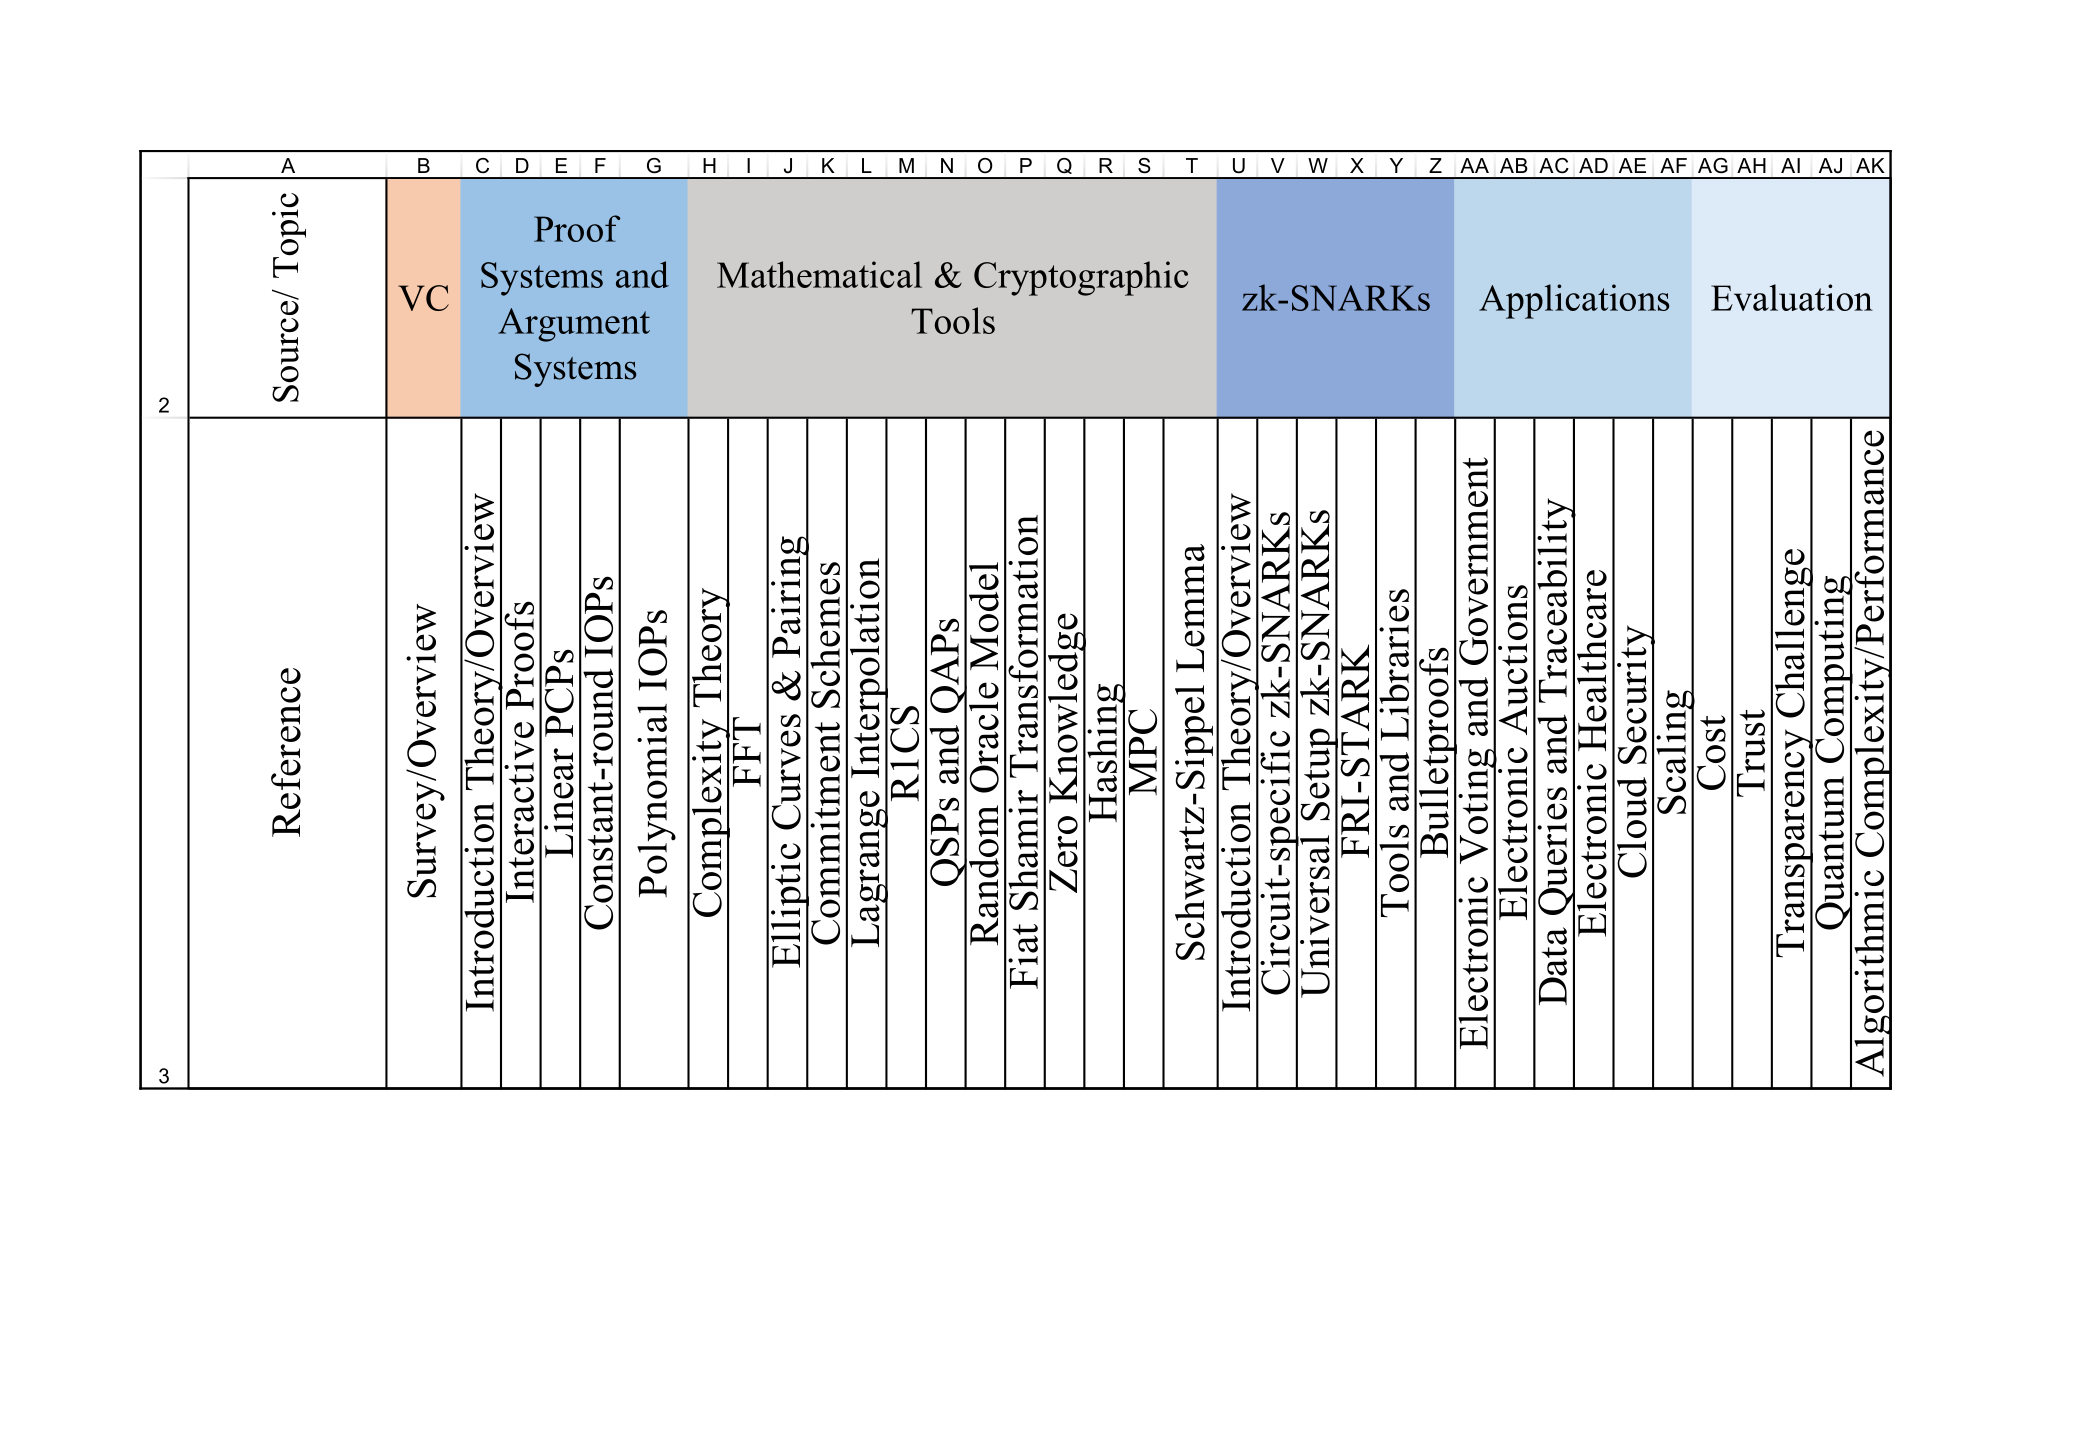
\includegraphics[width=1.0\textwidth]{Pictures/concept_matrix/wos-01.png}
\end{figure}

\begin{figure}[H]
	\centering
		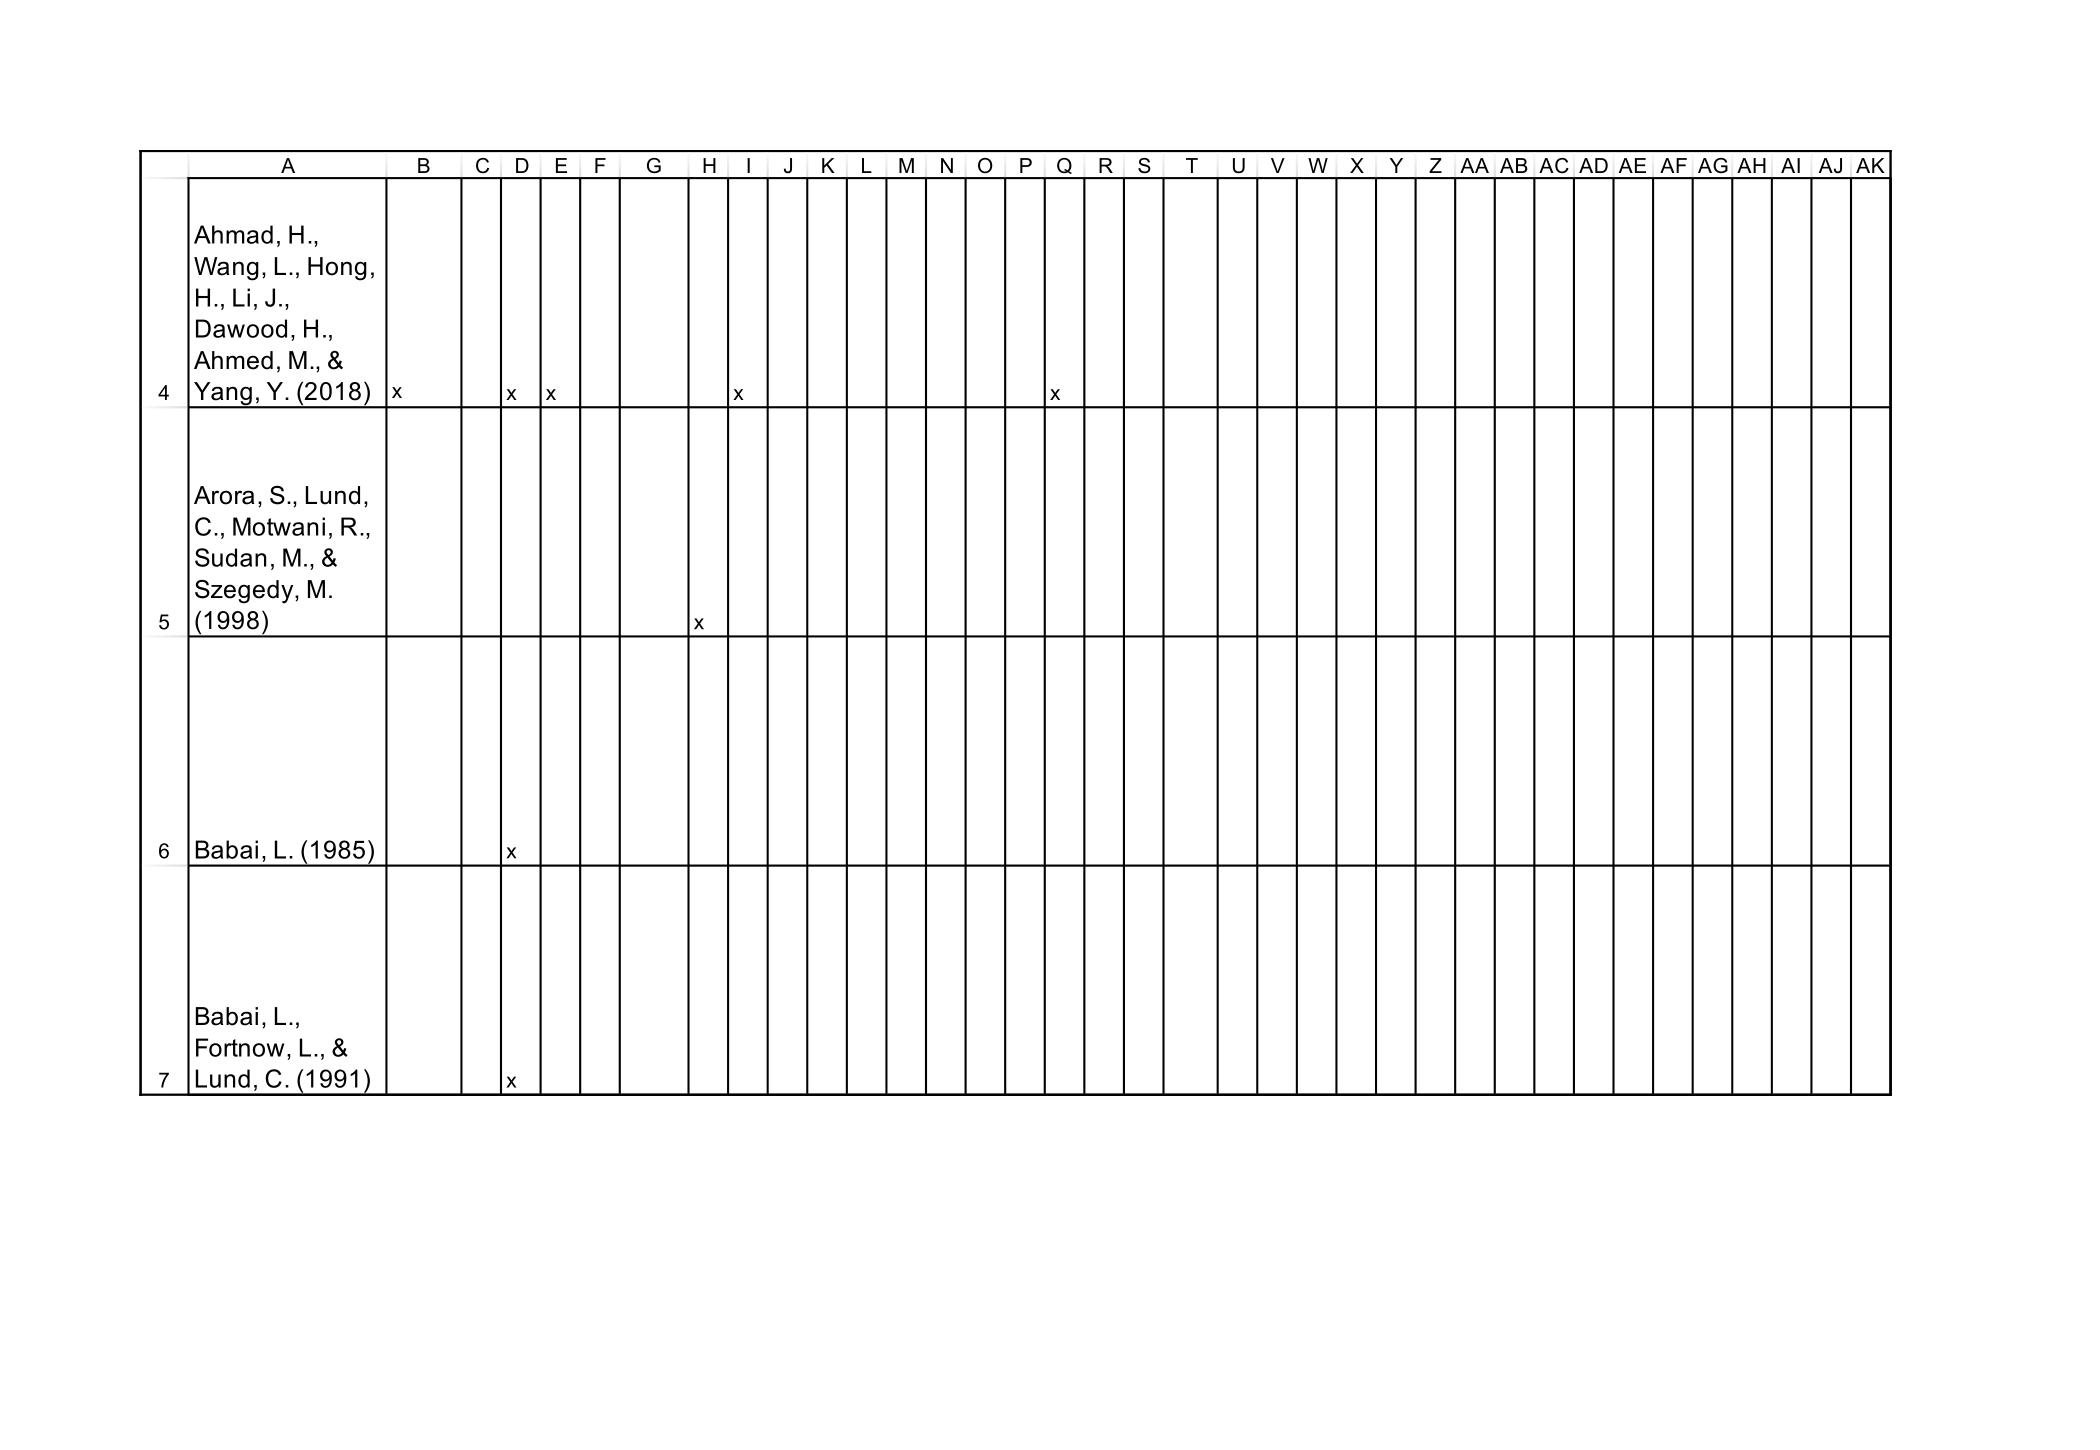
\includegraphics[width=.95\textwidth]{Pictures/concept_matrix/wos-02.png}
\end{figure}
\begin{figure}[H]
	\centering
		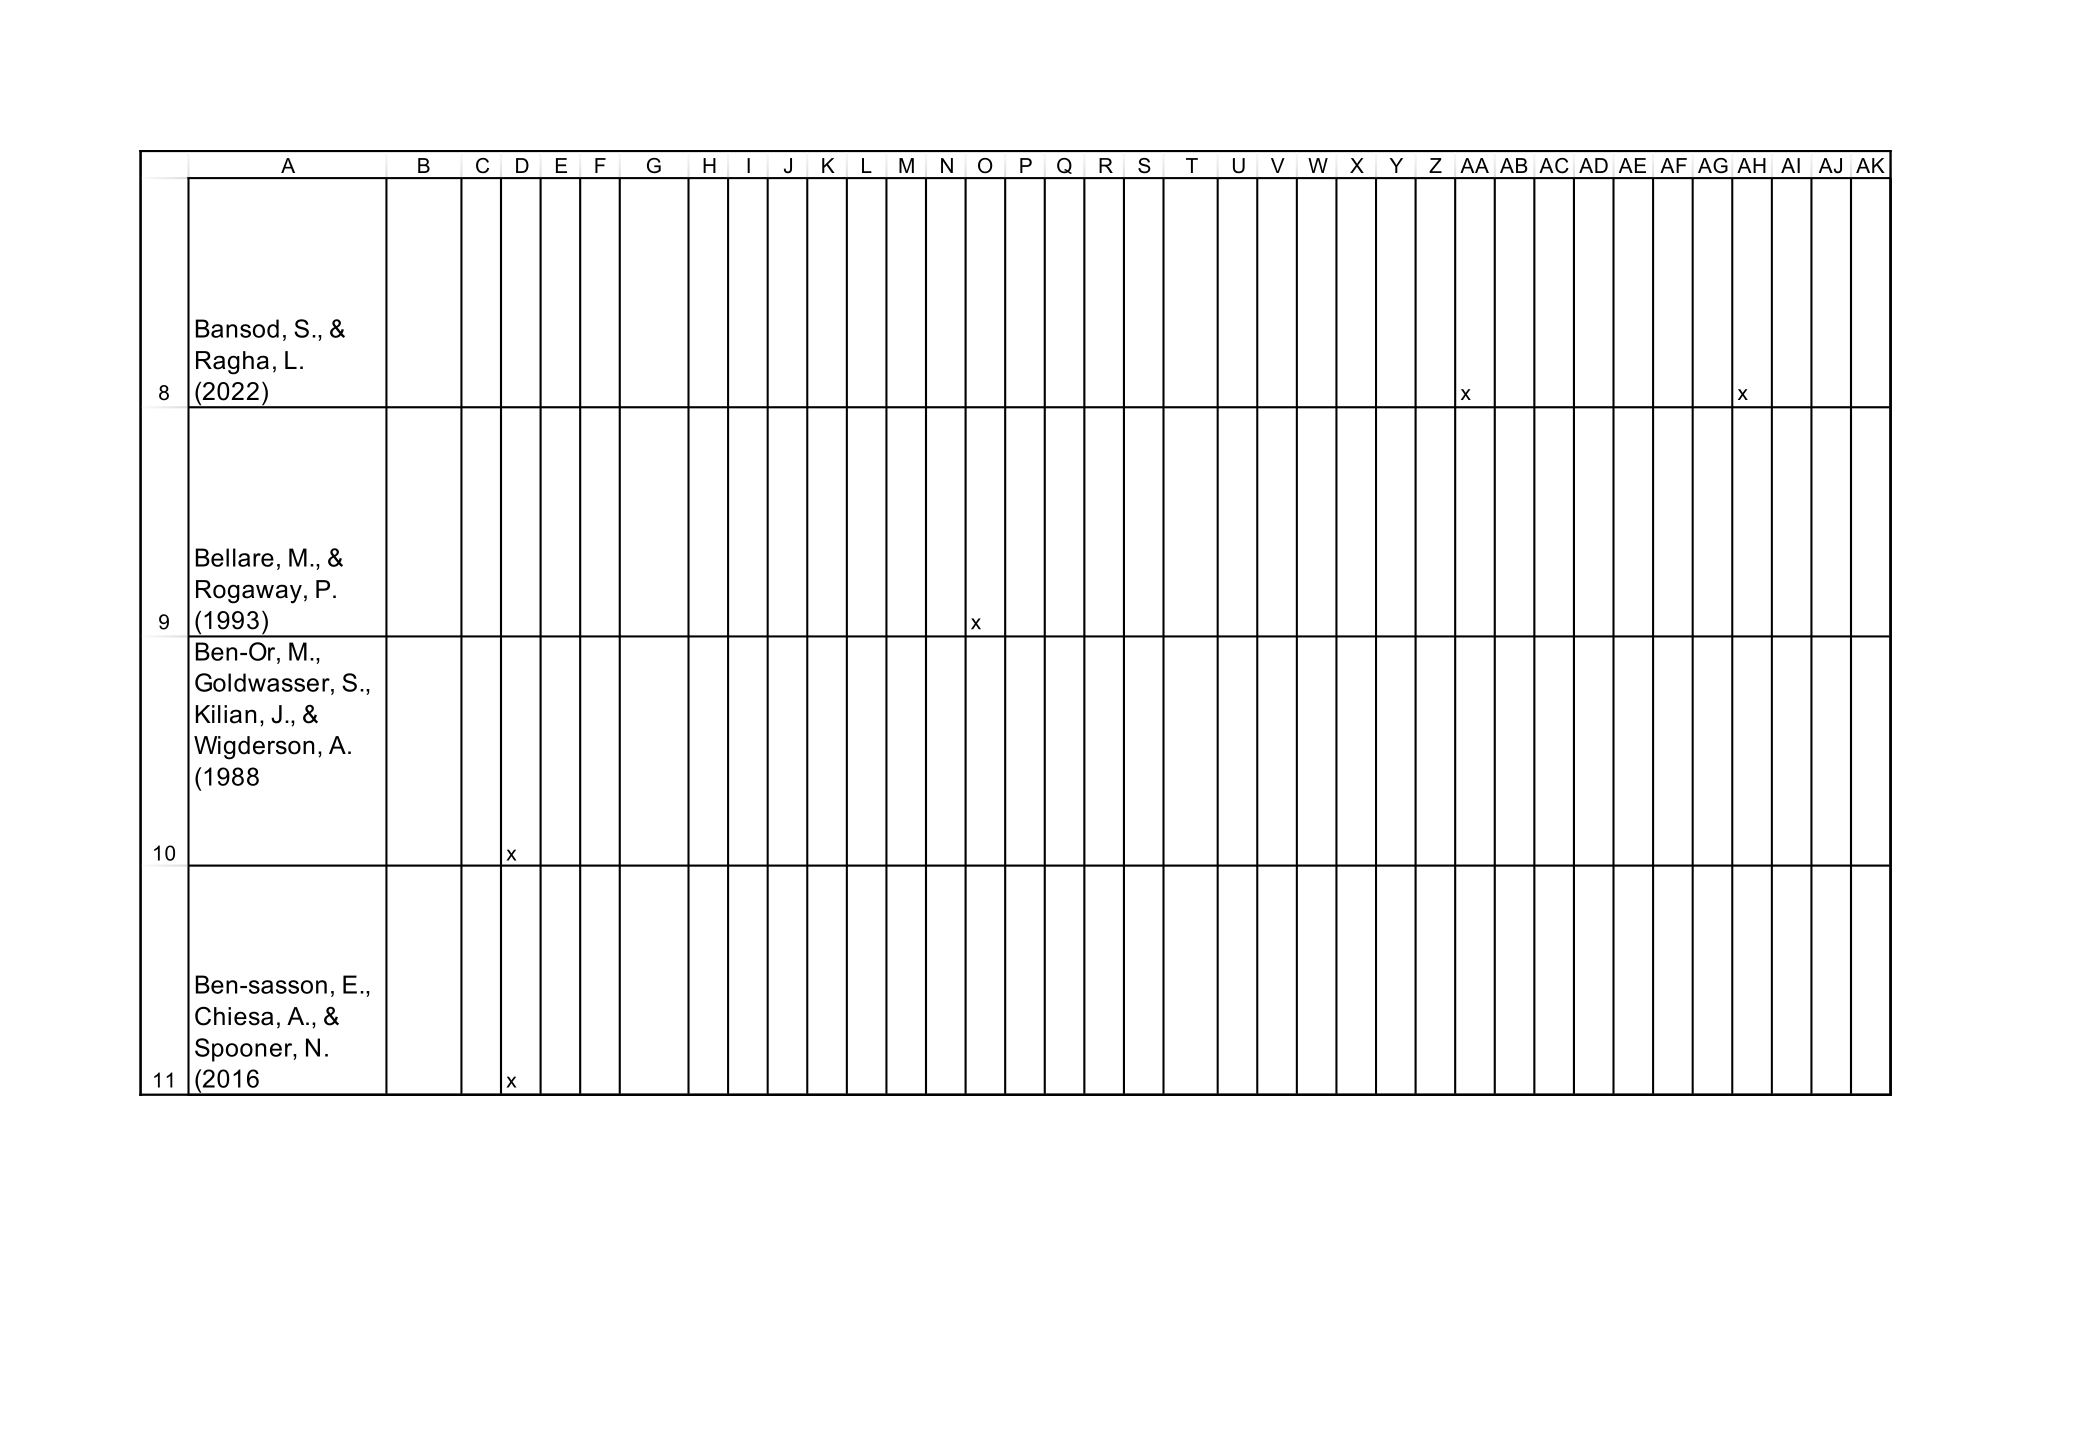
\includegraphics[width=.95\textwidth]{Pictures/concept_matrix/wos-03.png}
\end{figure}
\begin{figure}[H]
	\centering
		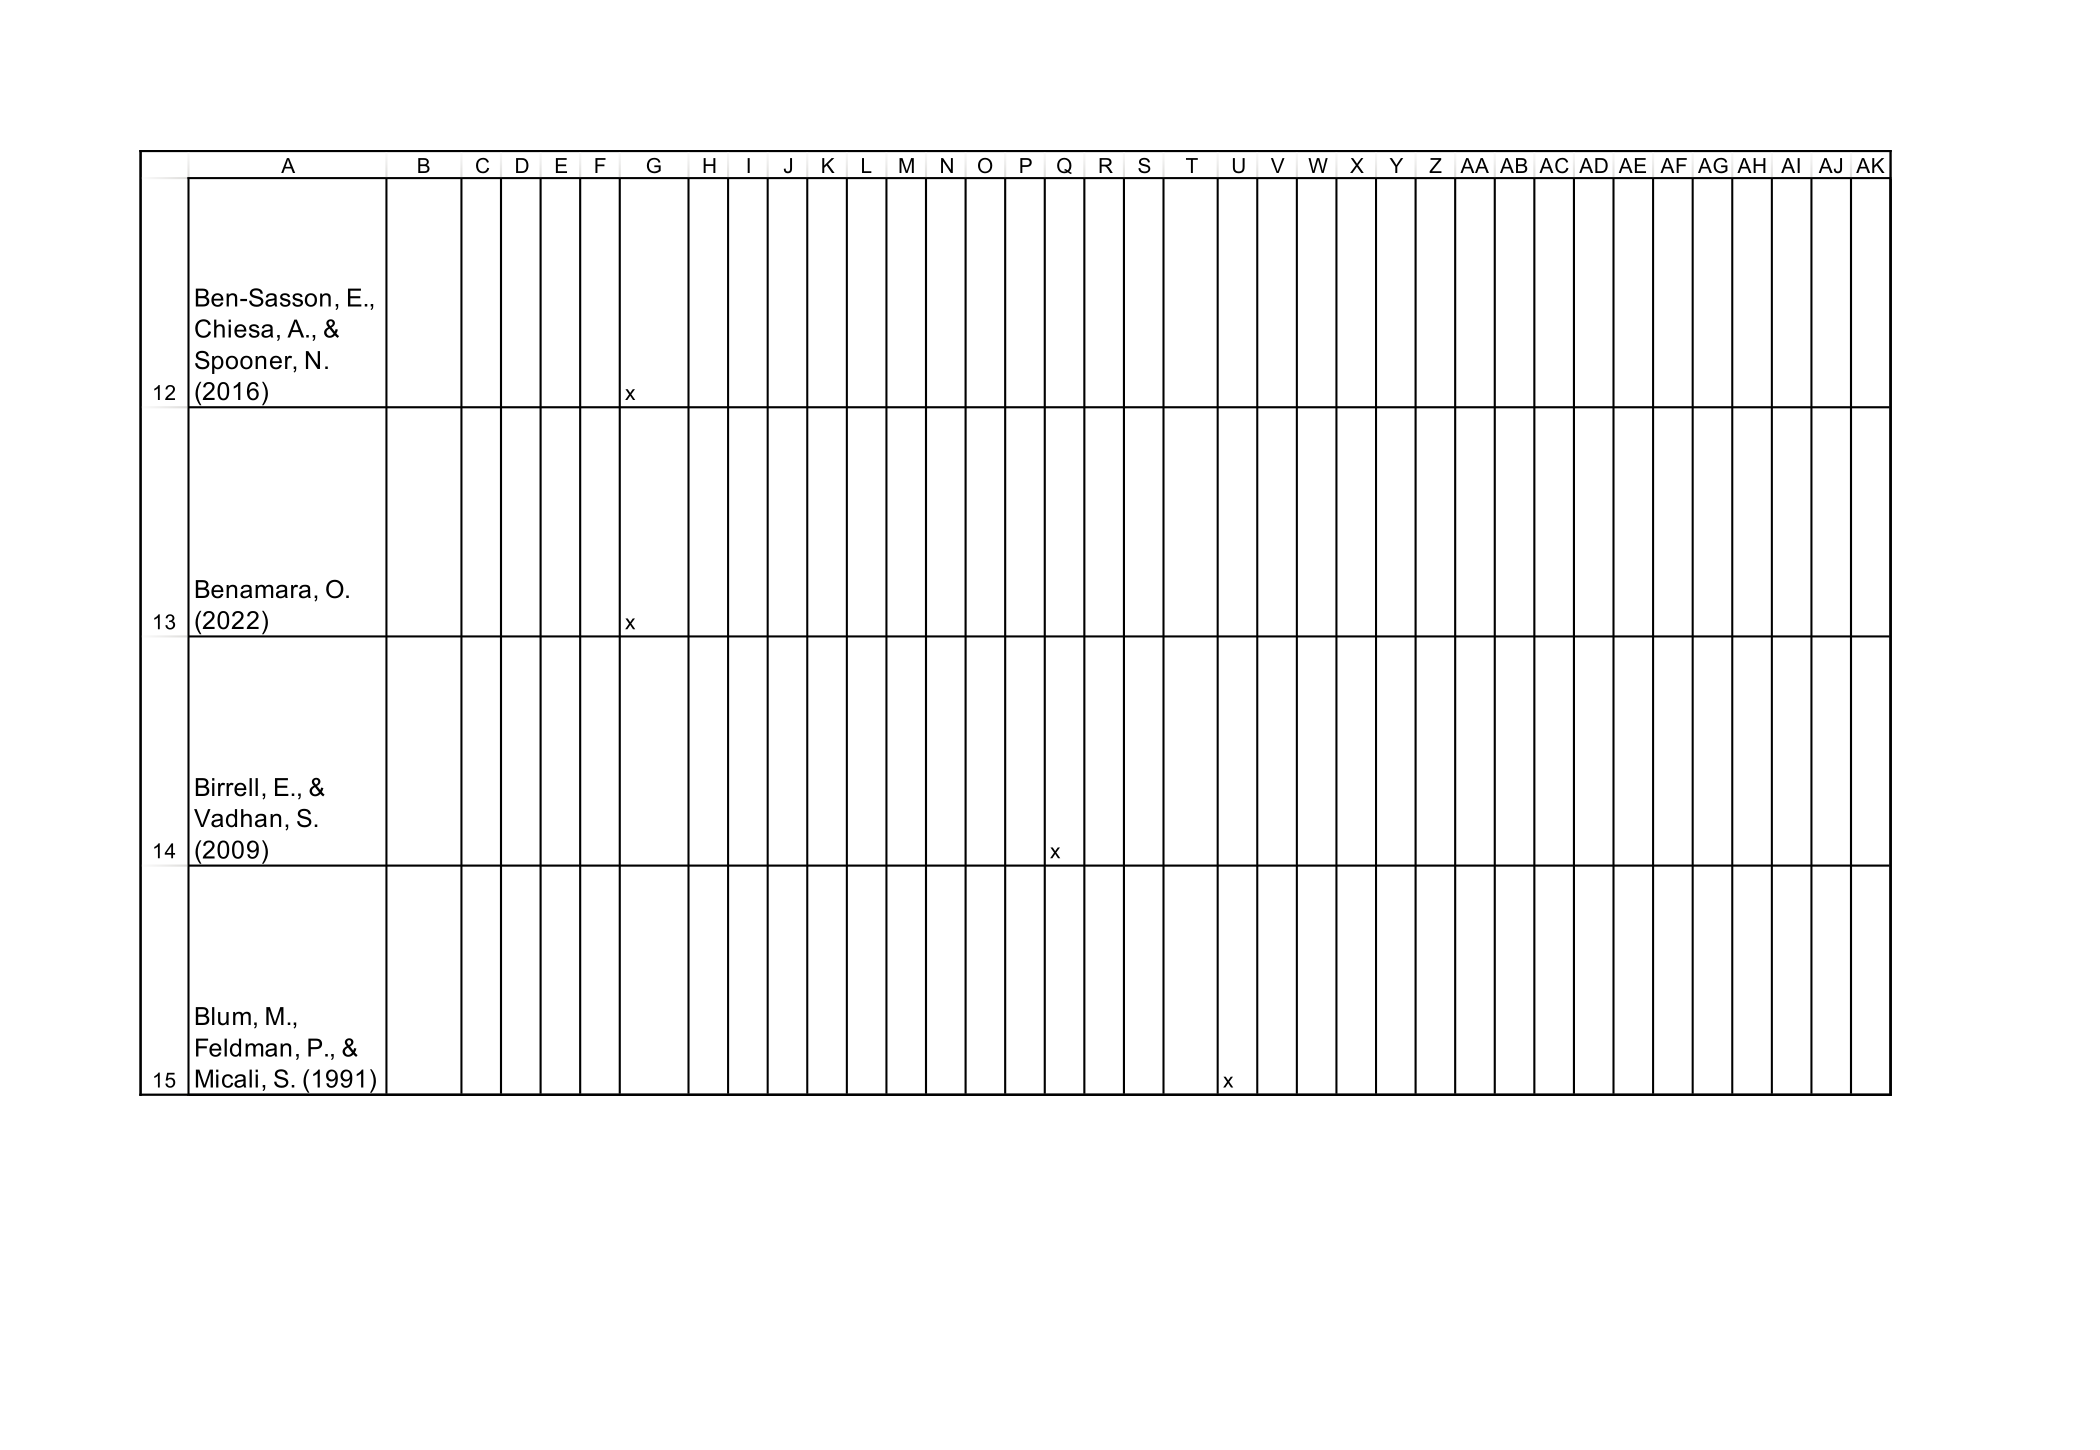
\includegraphics[width=.95\textwidth]{Pictures/concept_matrix/wos-04.png}
\end{figure}
\begin{figure}[H]
	\centering
		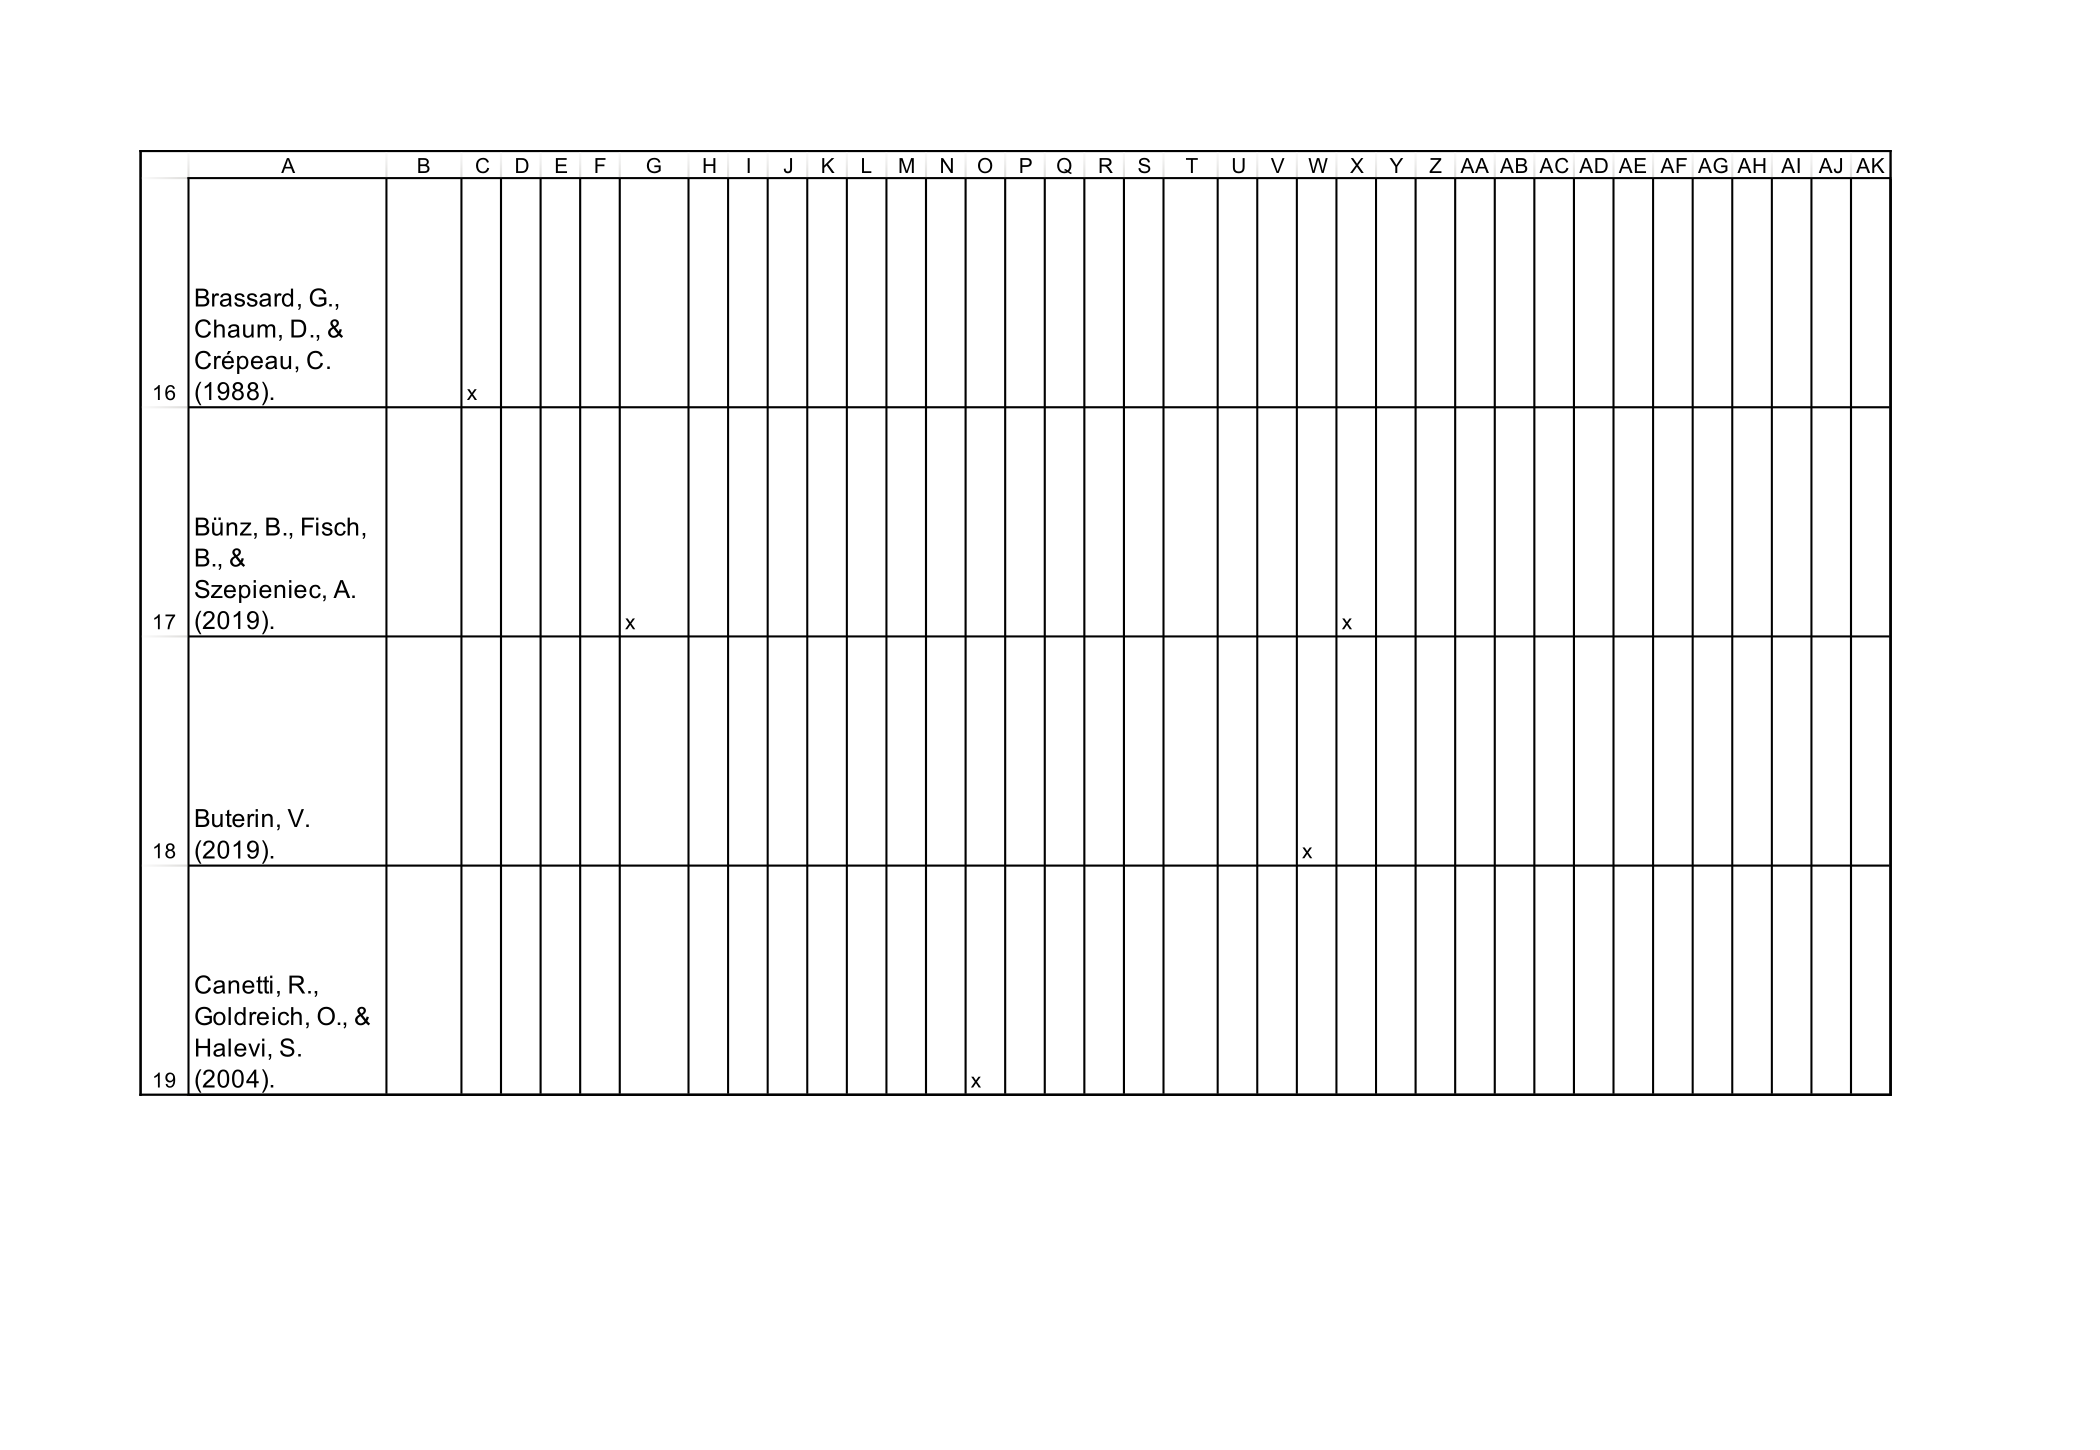
\includegraphics[width=.95\textwidth]{Pictures/concept_matrix/wos-05.png}
\end{figure}

\begin{figure}[H]
	\centering
		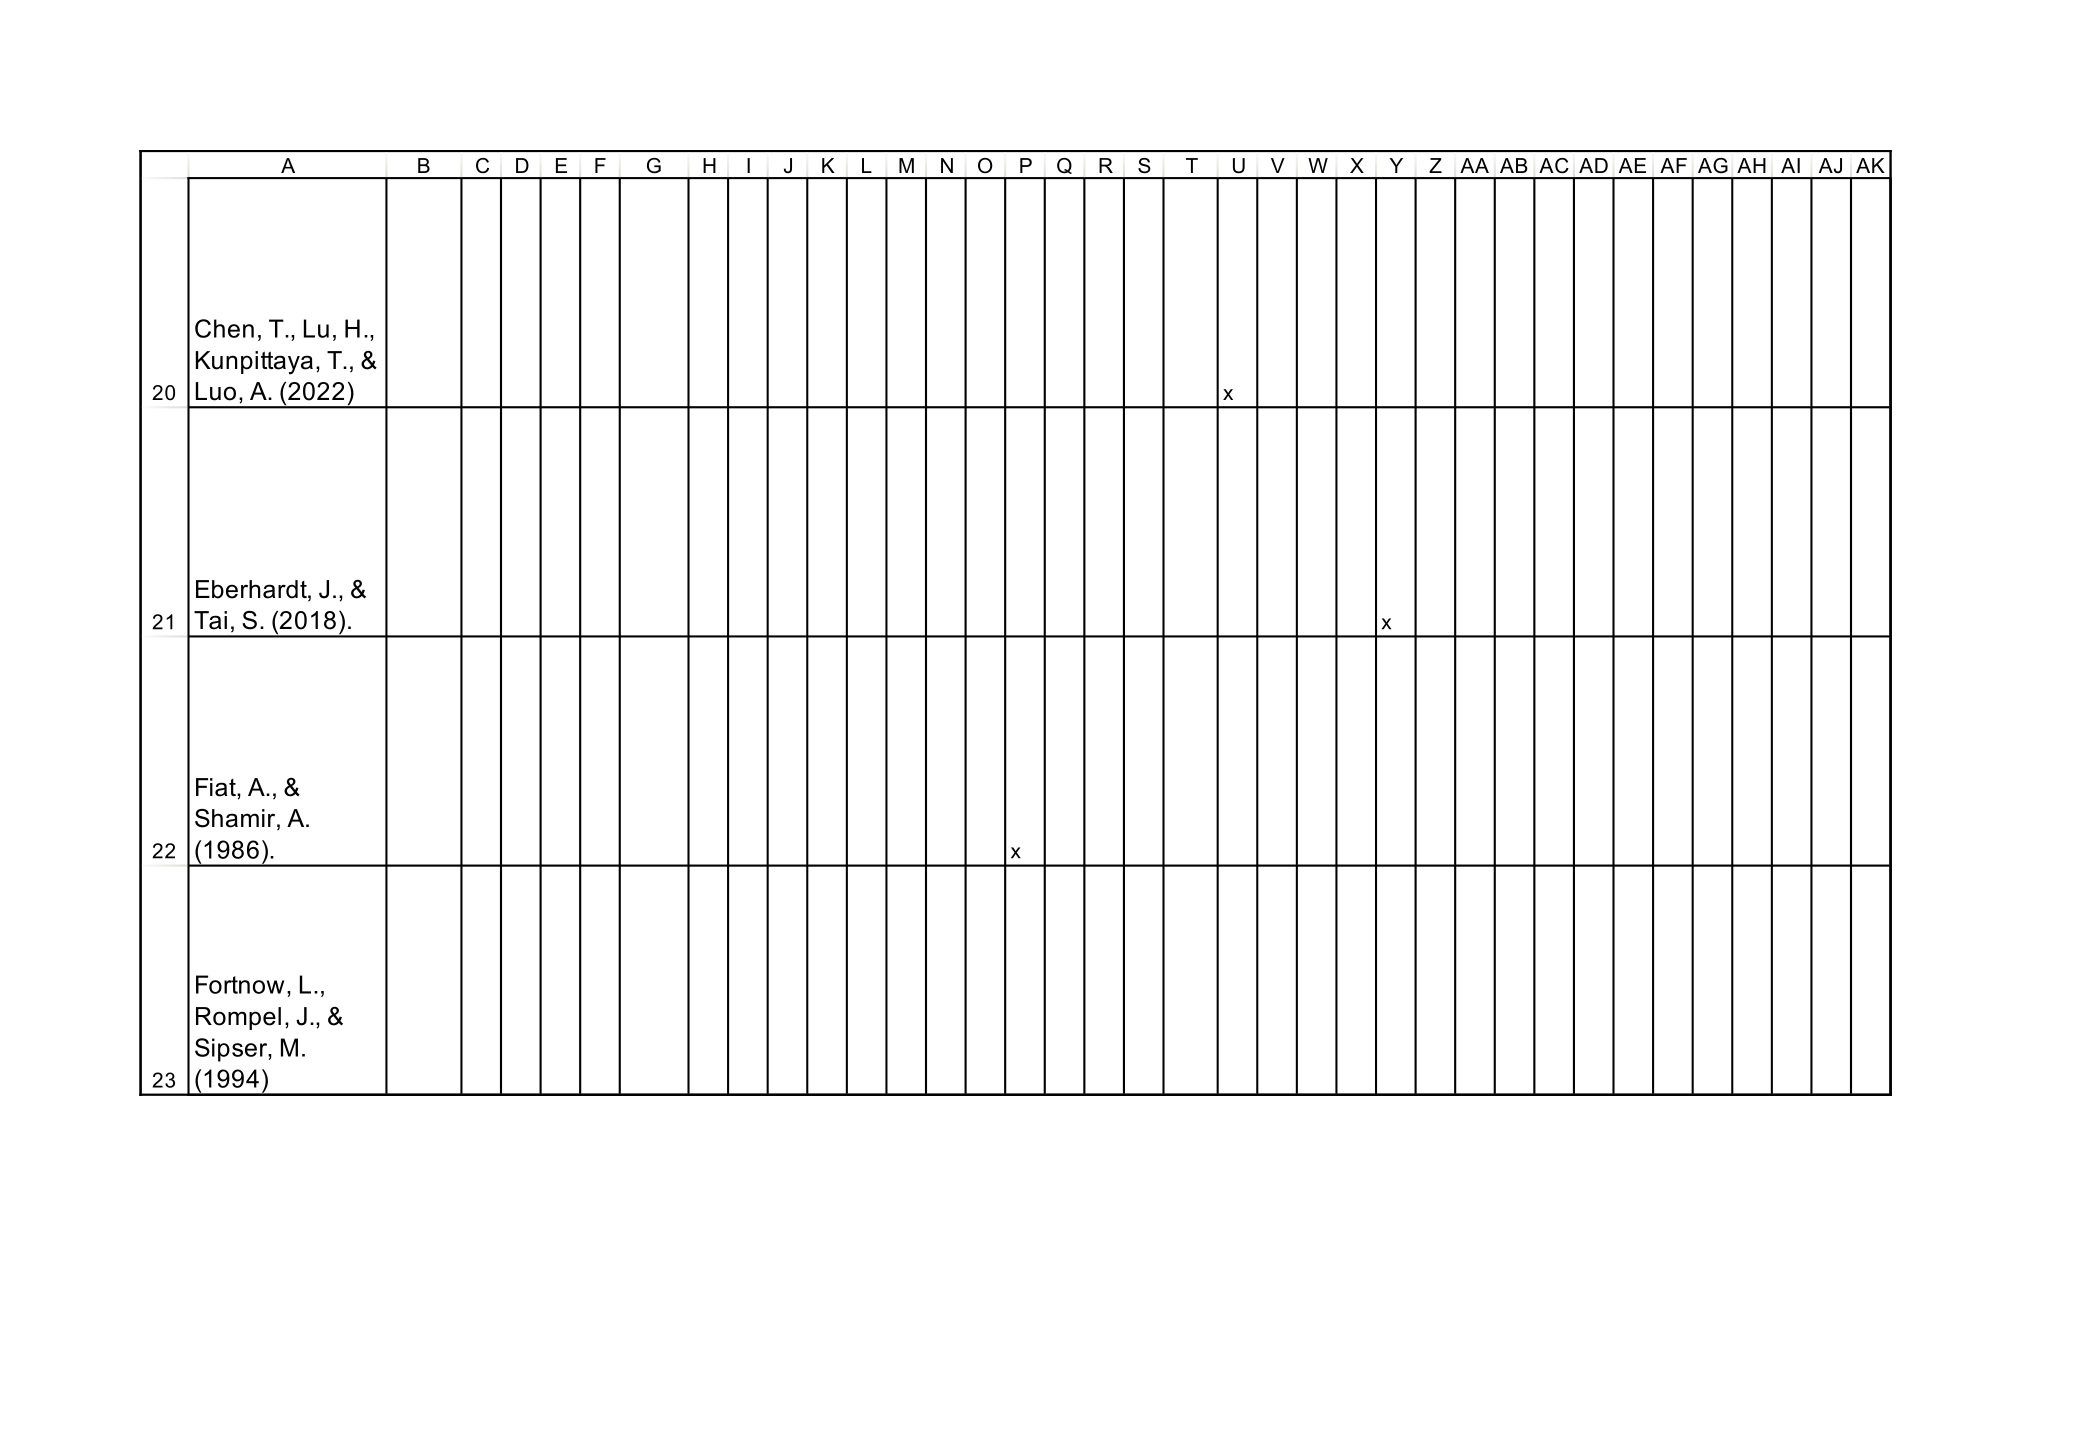
\includegraphics[width=.95\textwidth]{Pictures/concept_matrix/wos-06.png}
\end{figure}

\begin{figure}[H]
	\centering
		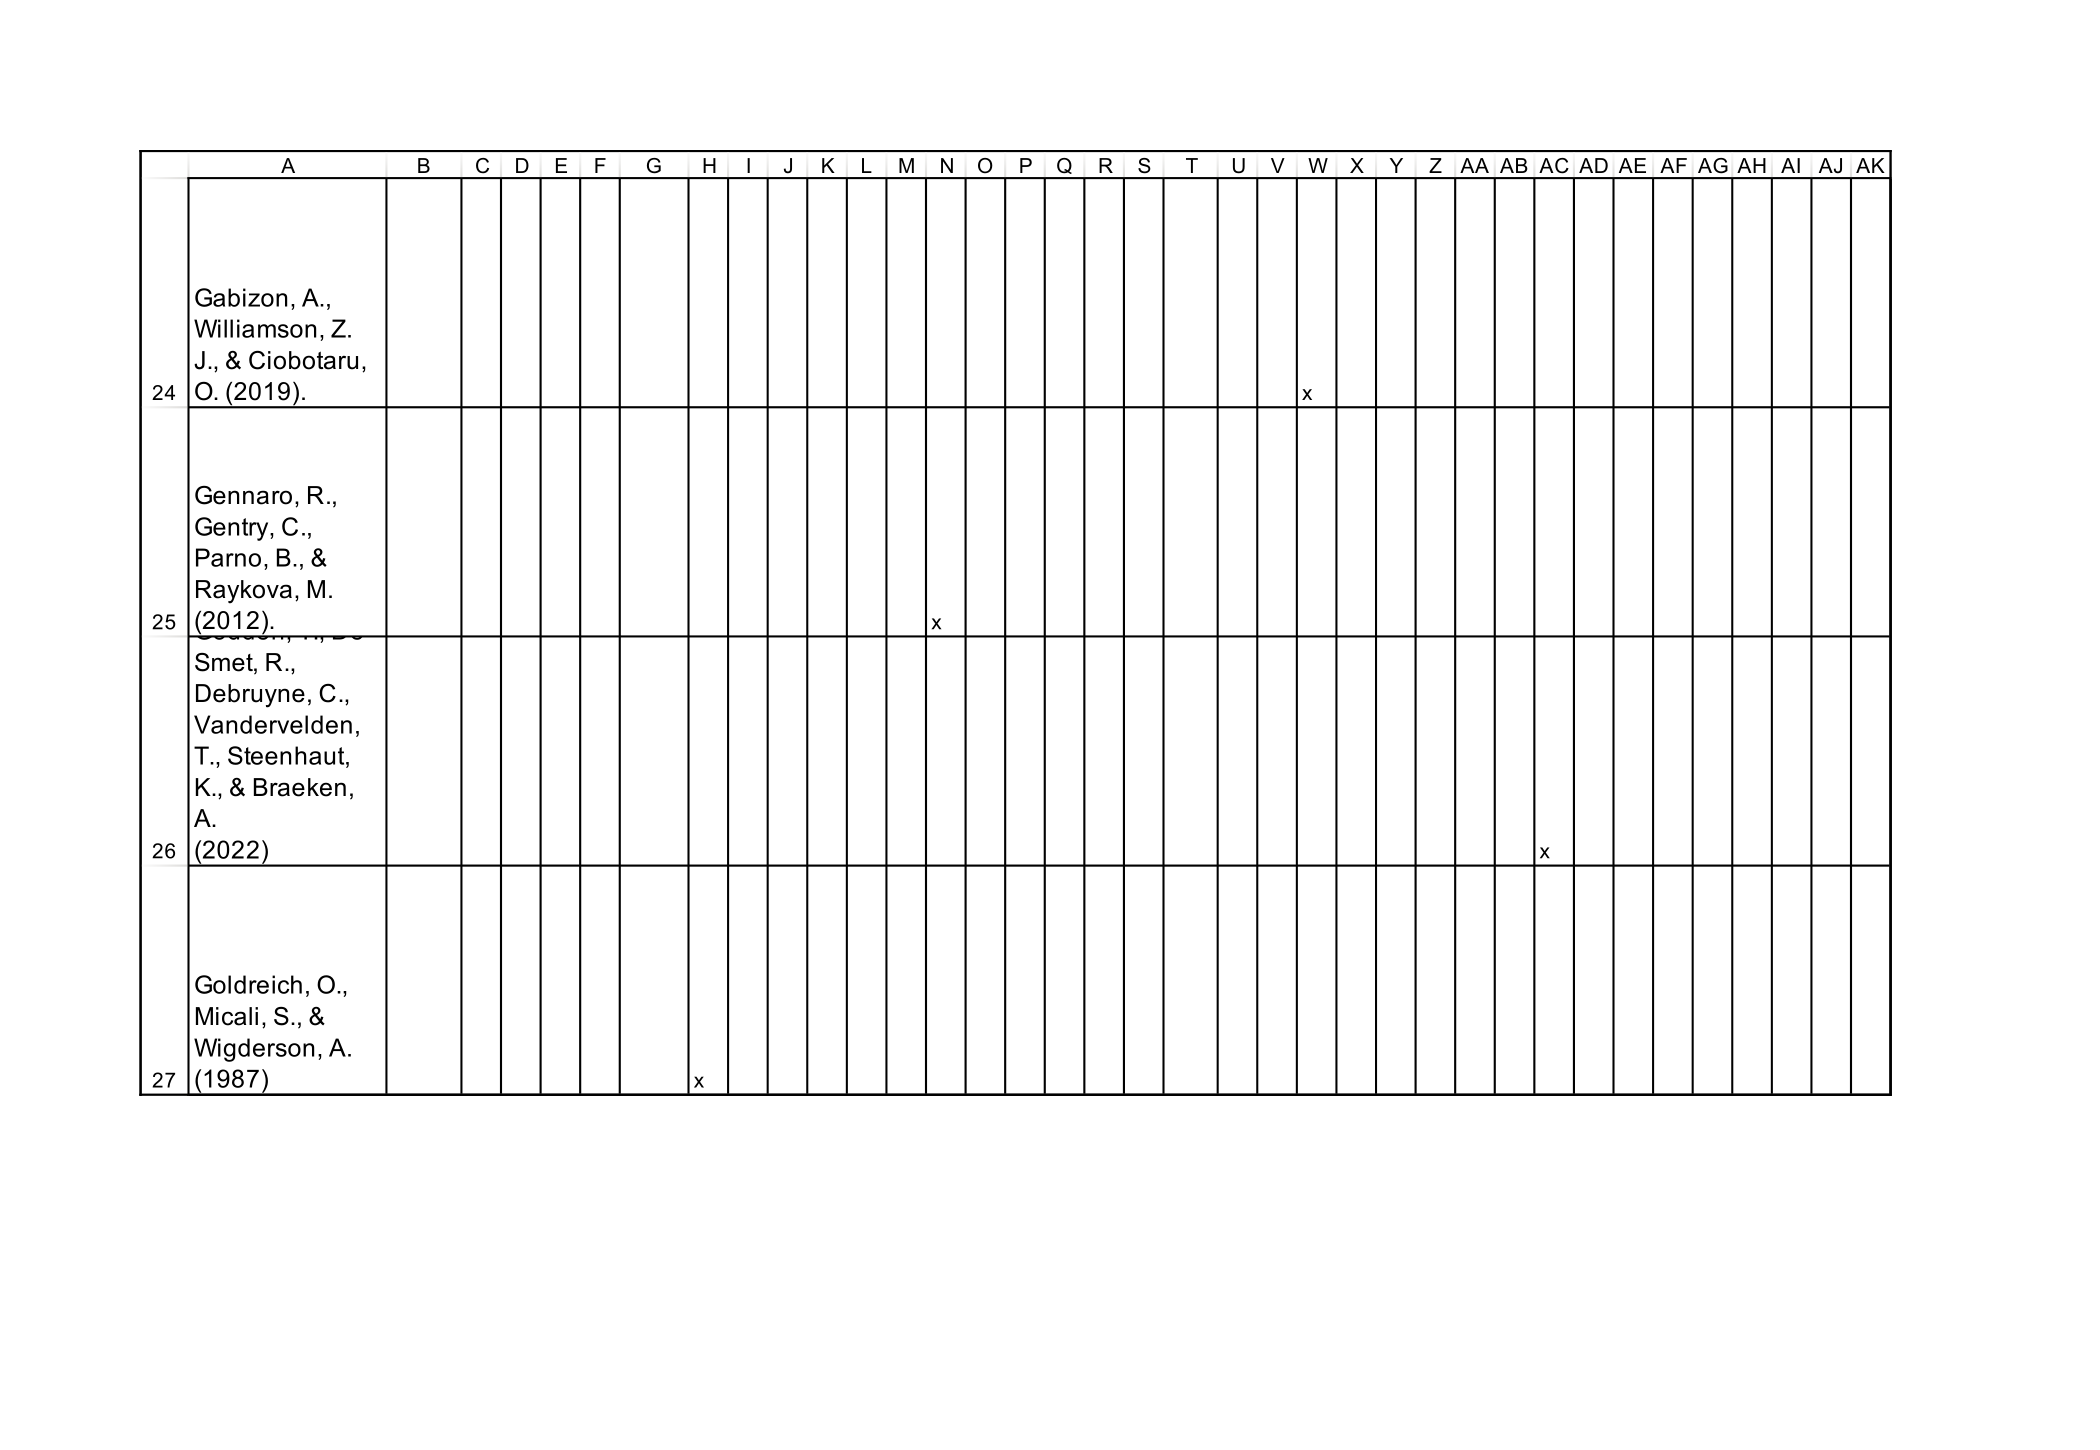
\includegraphics[width=.95\textwidth]{Pictures/concept_matrix/wos-07.png}
\end{figure}

\begin{figure}[H]
	\centering
		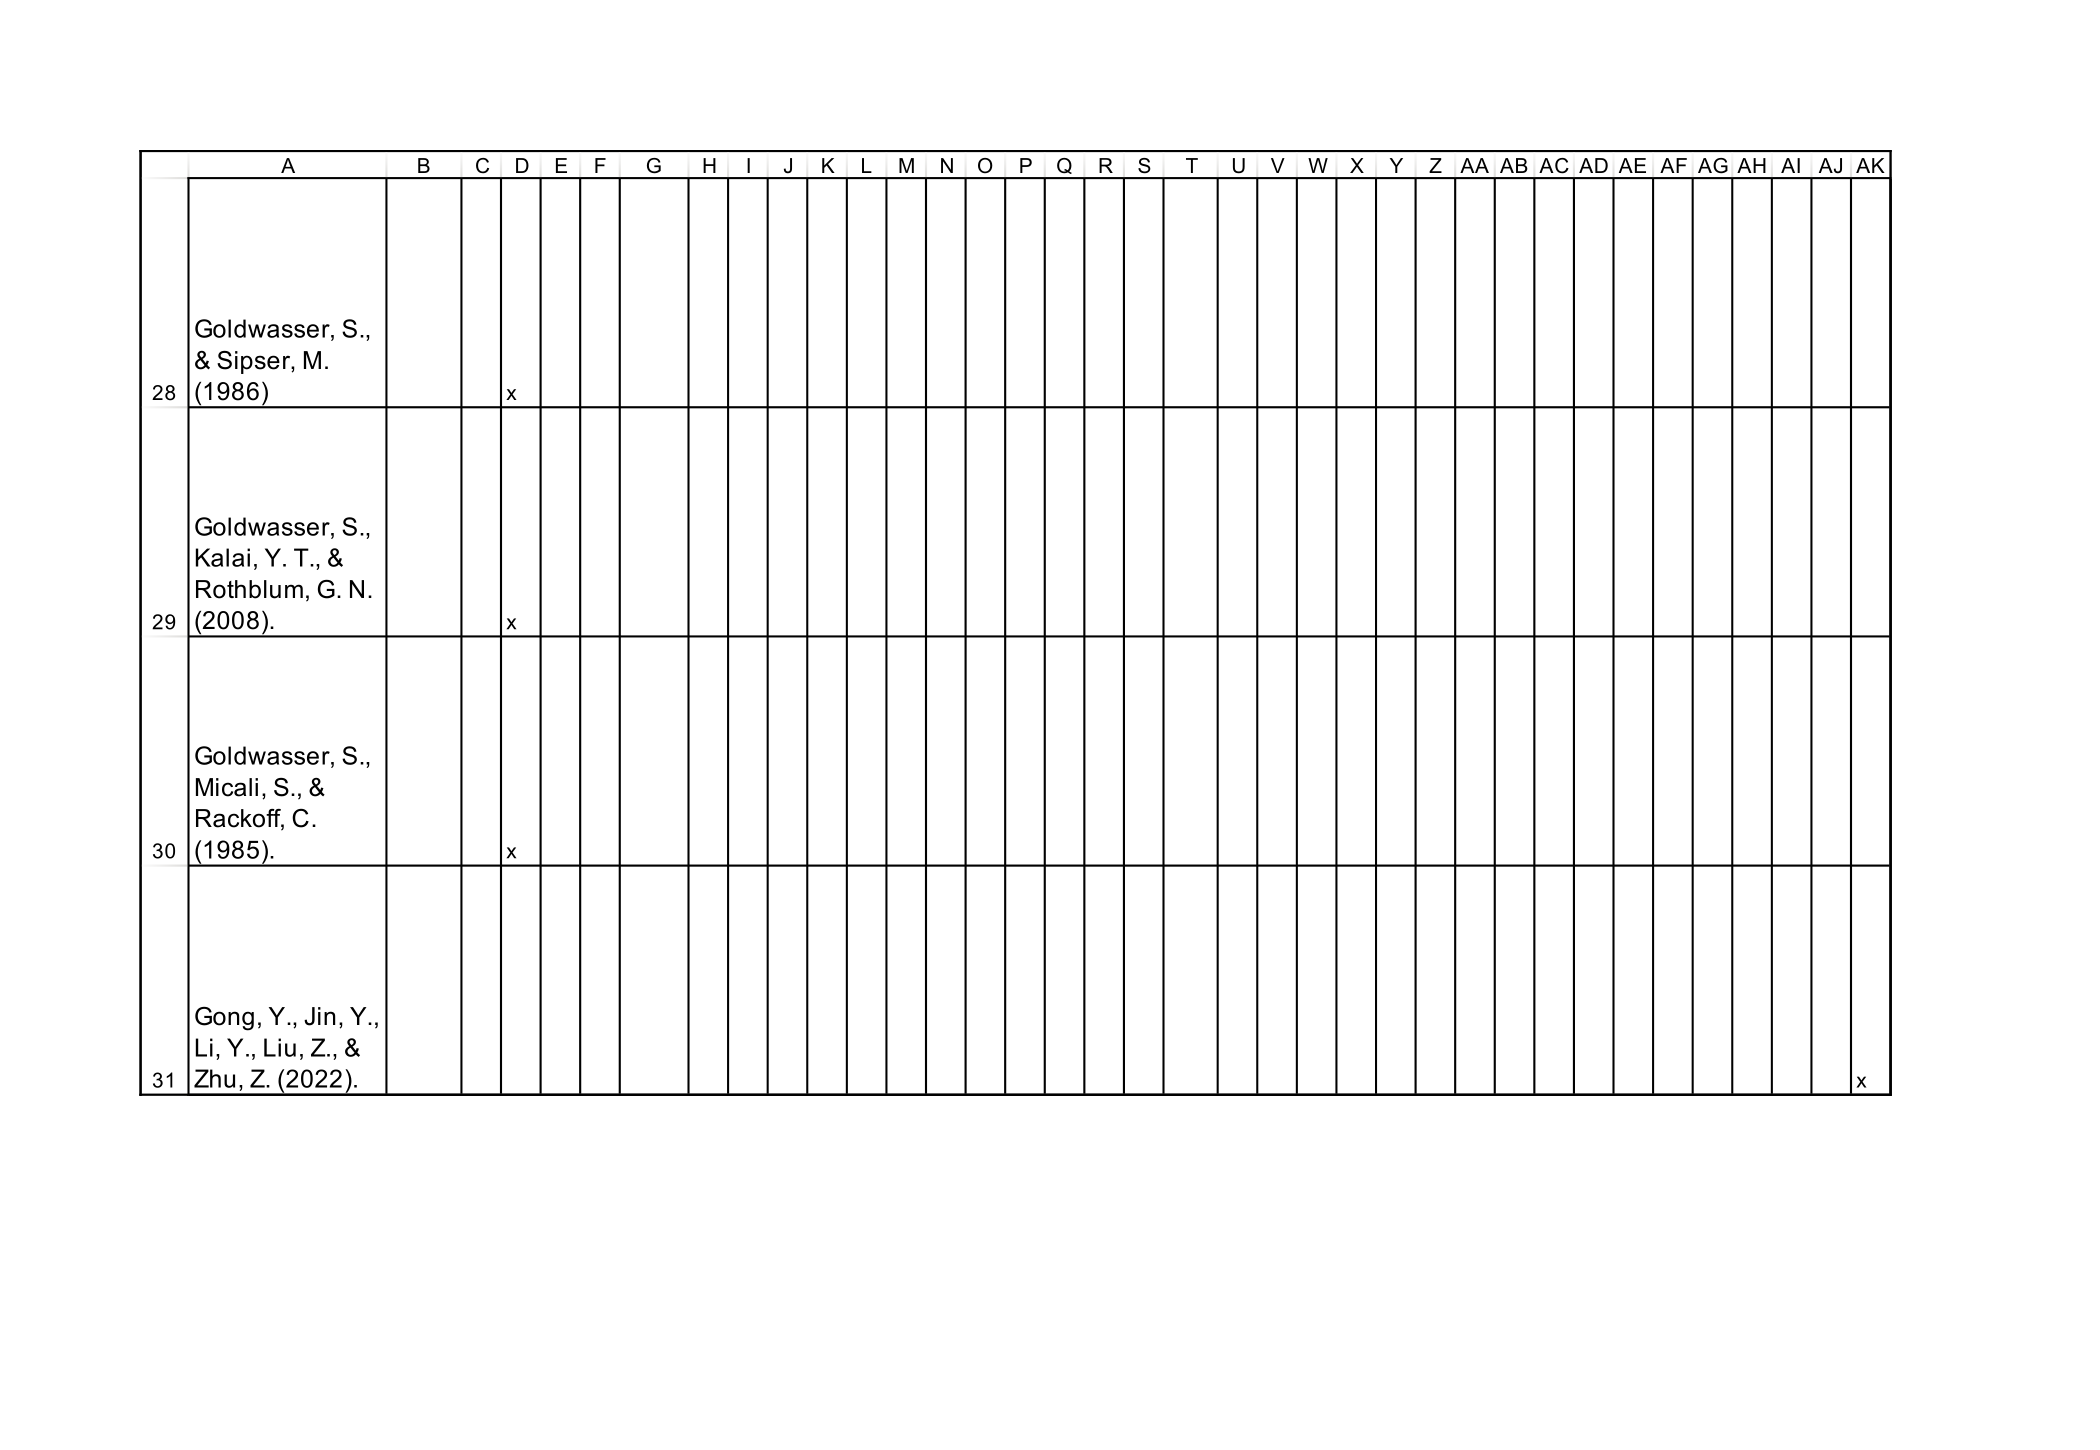
\includegraphics[width=.95\textwidth]{Pictures/concept_matrix/wos-08.png}
\end{figure}

\begin{figure}[H]
	\centering
		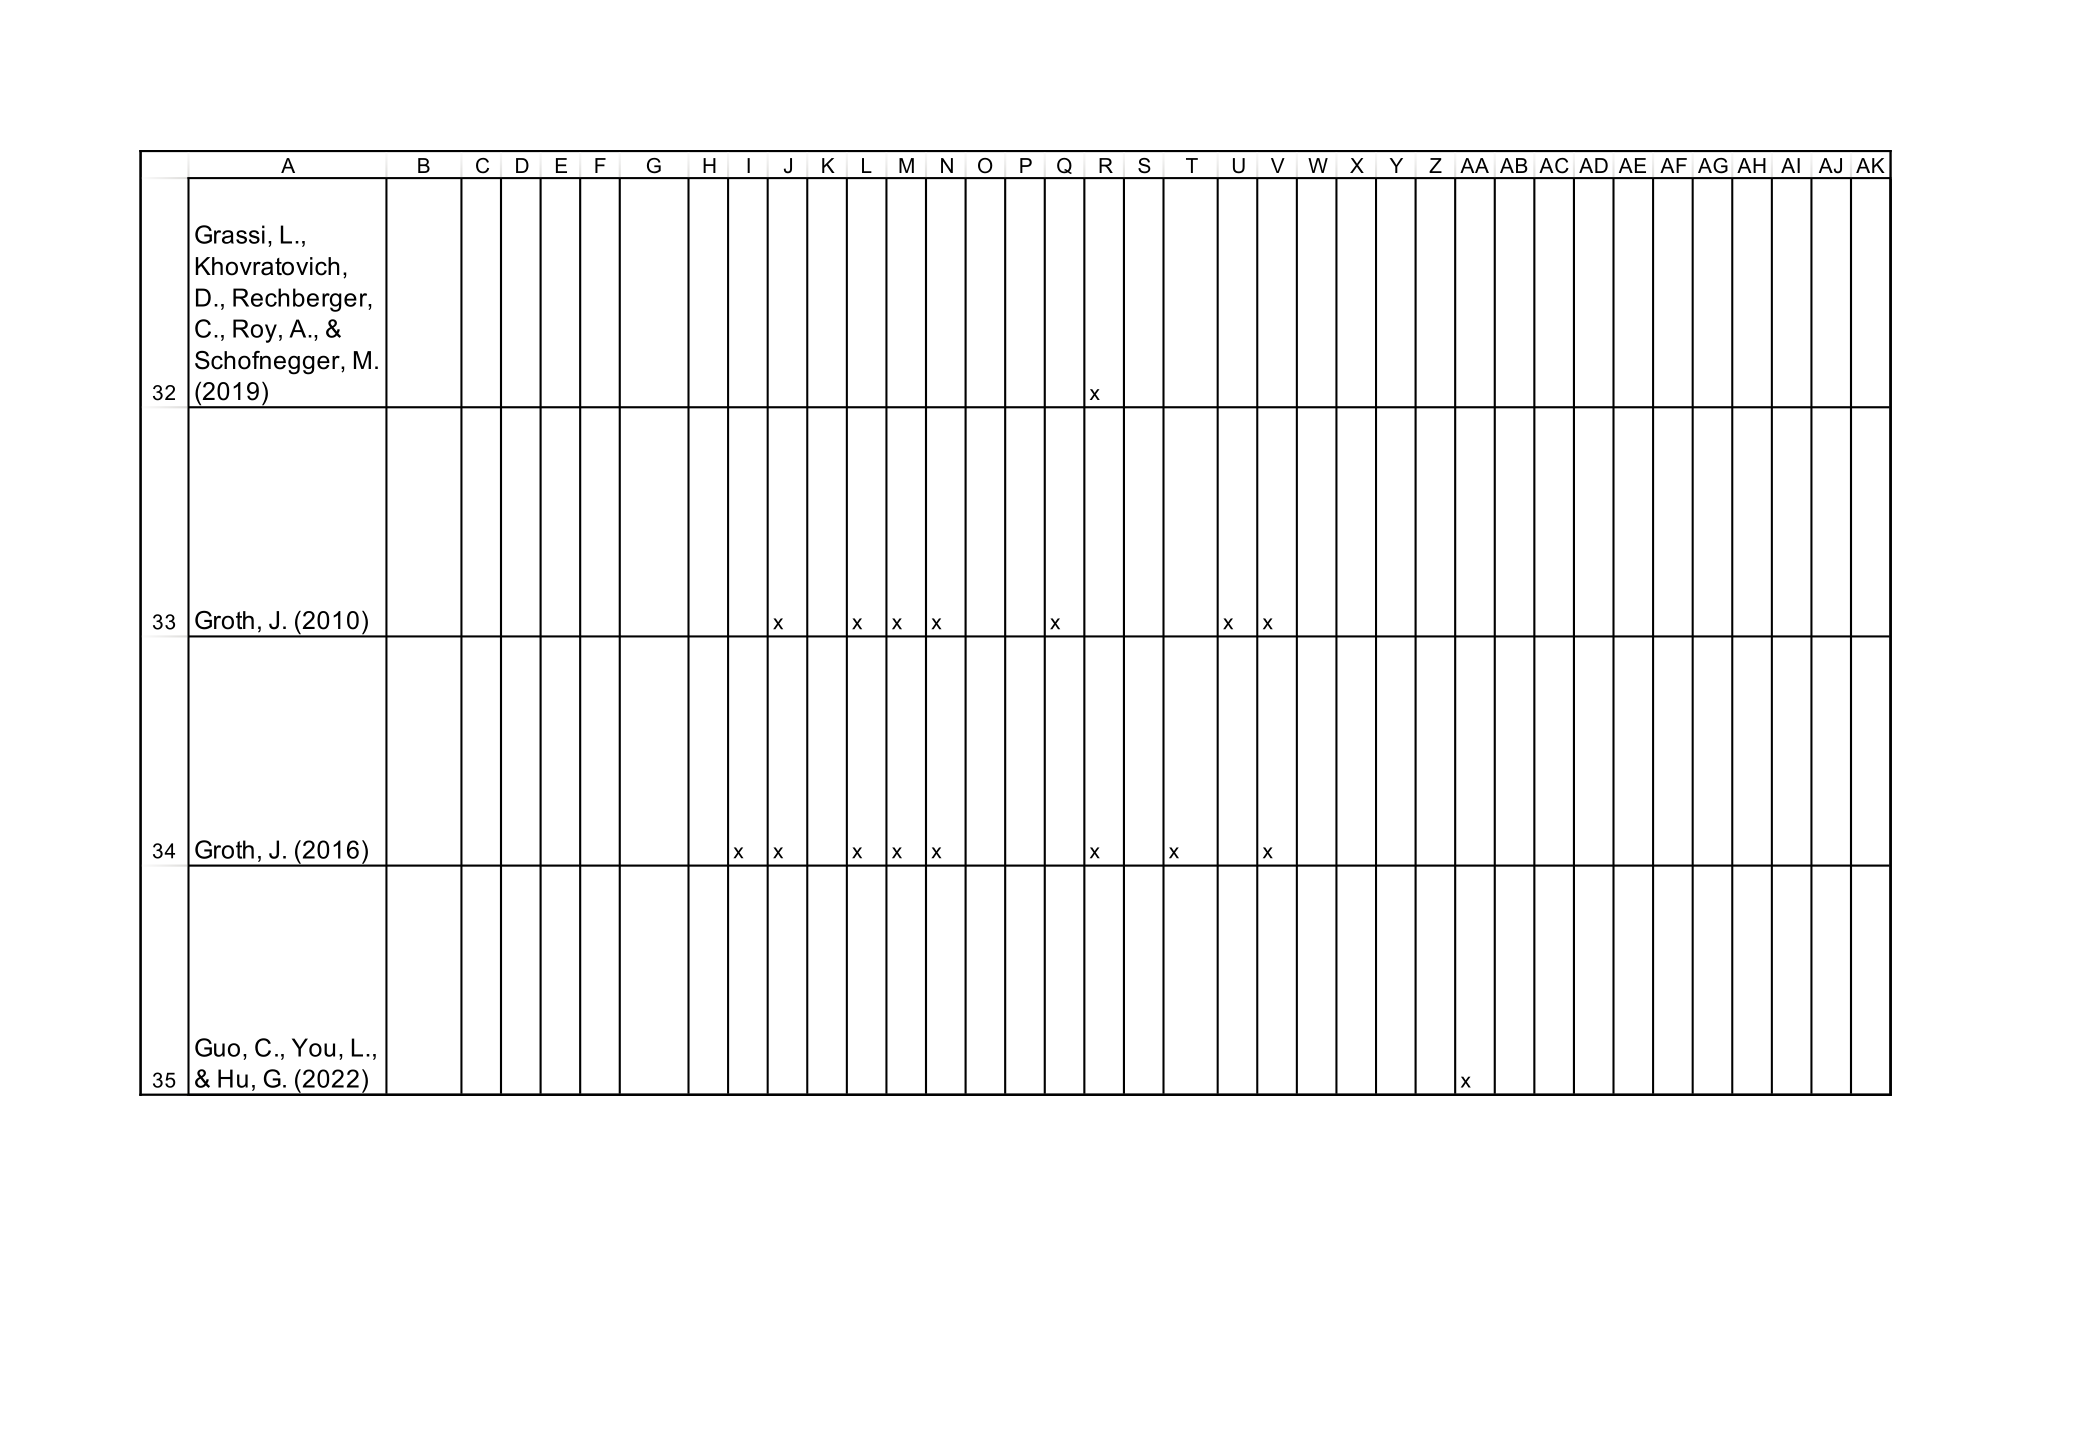
\includegraphics[width=.95\textwidth]{Pictures/concept_matrix/wos-09.png}
\end{figure}

\begin{figure}[H]
	\centering
		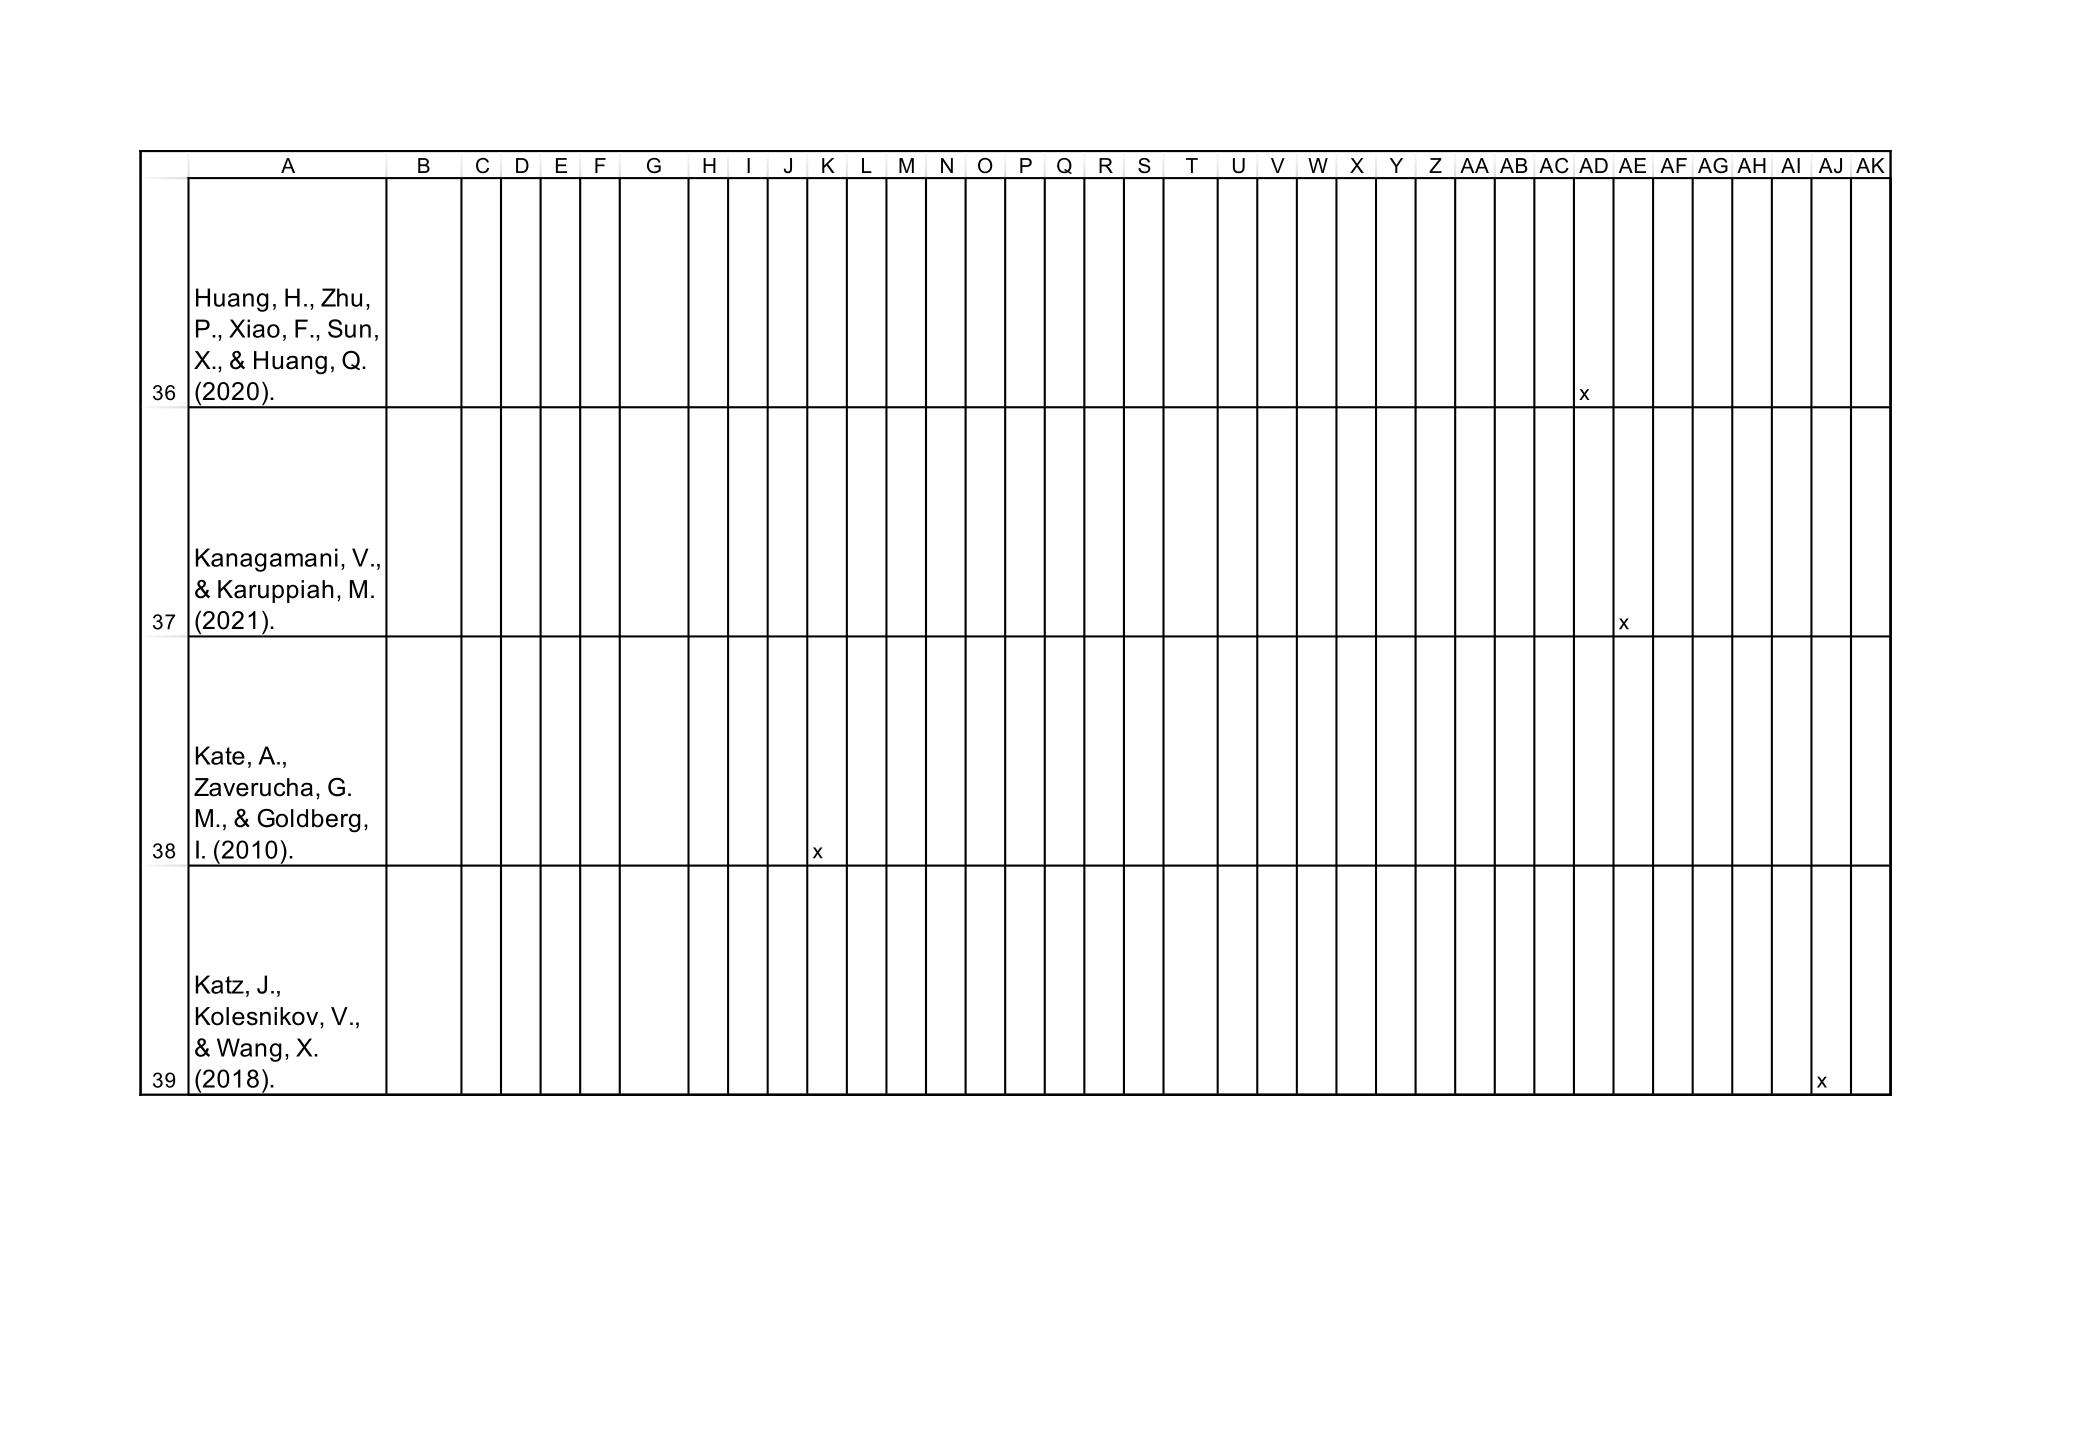
\includegraphics[width=.95\textwidth]{Pictures/concept_matrix/wos-10.png}
\end{figure}

\begin{figure}[H]
	\centering
		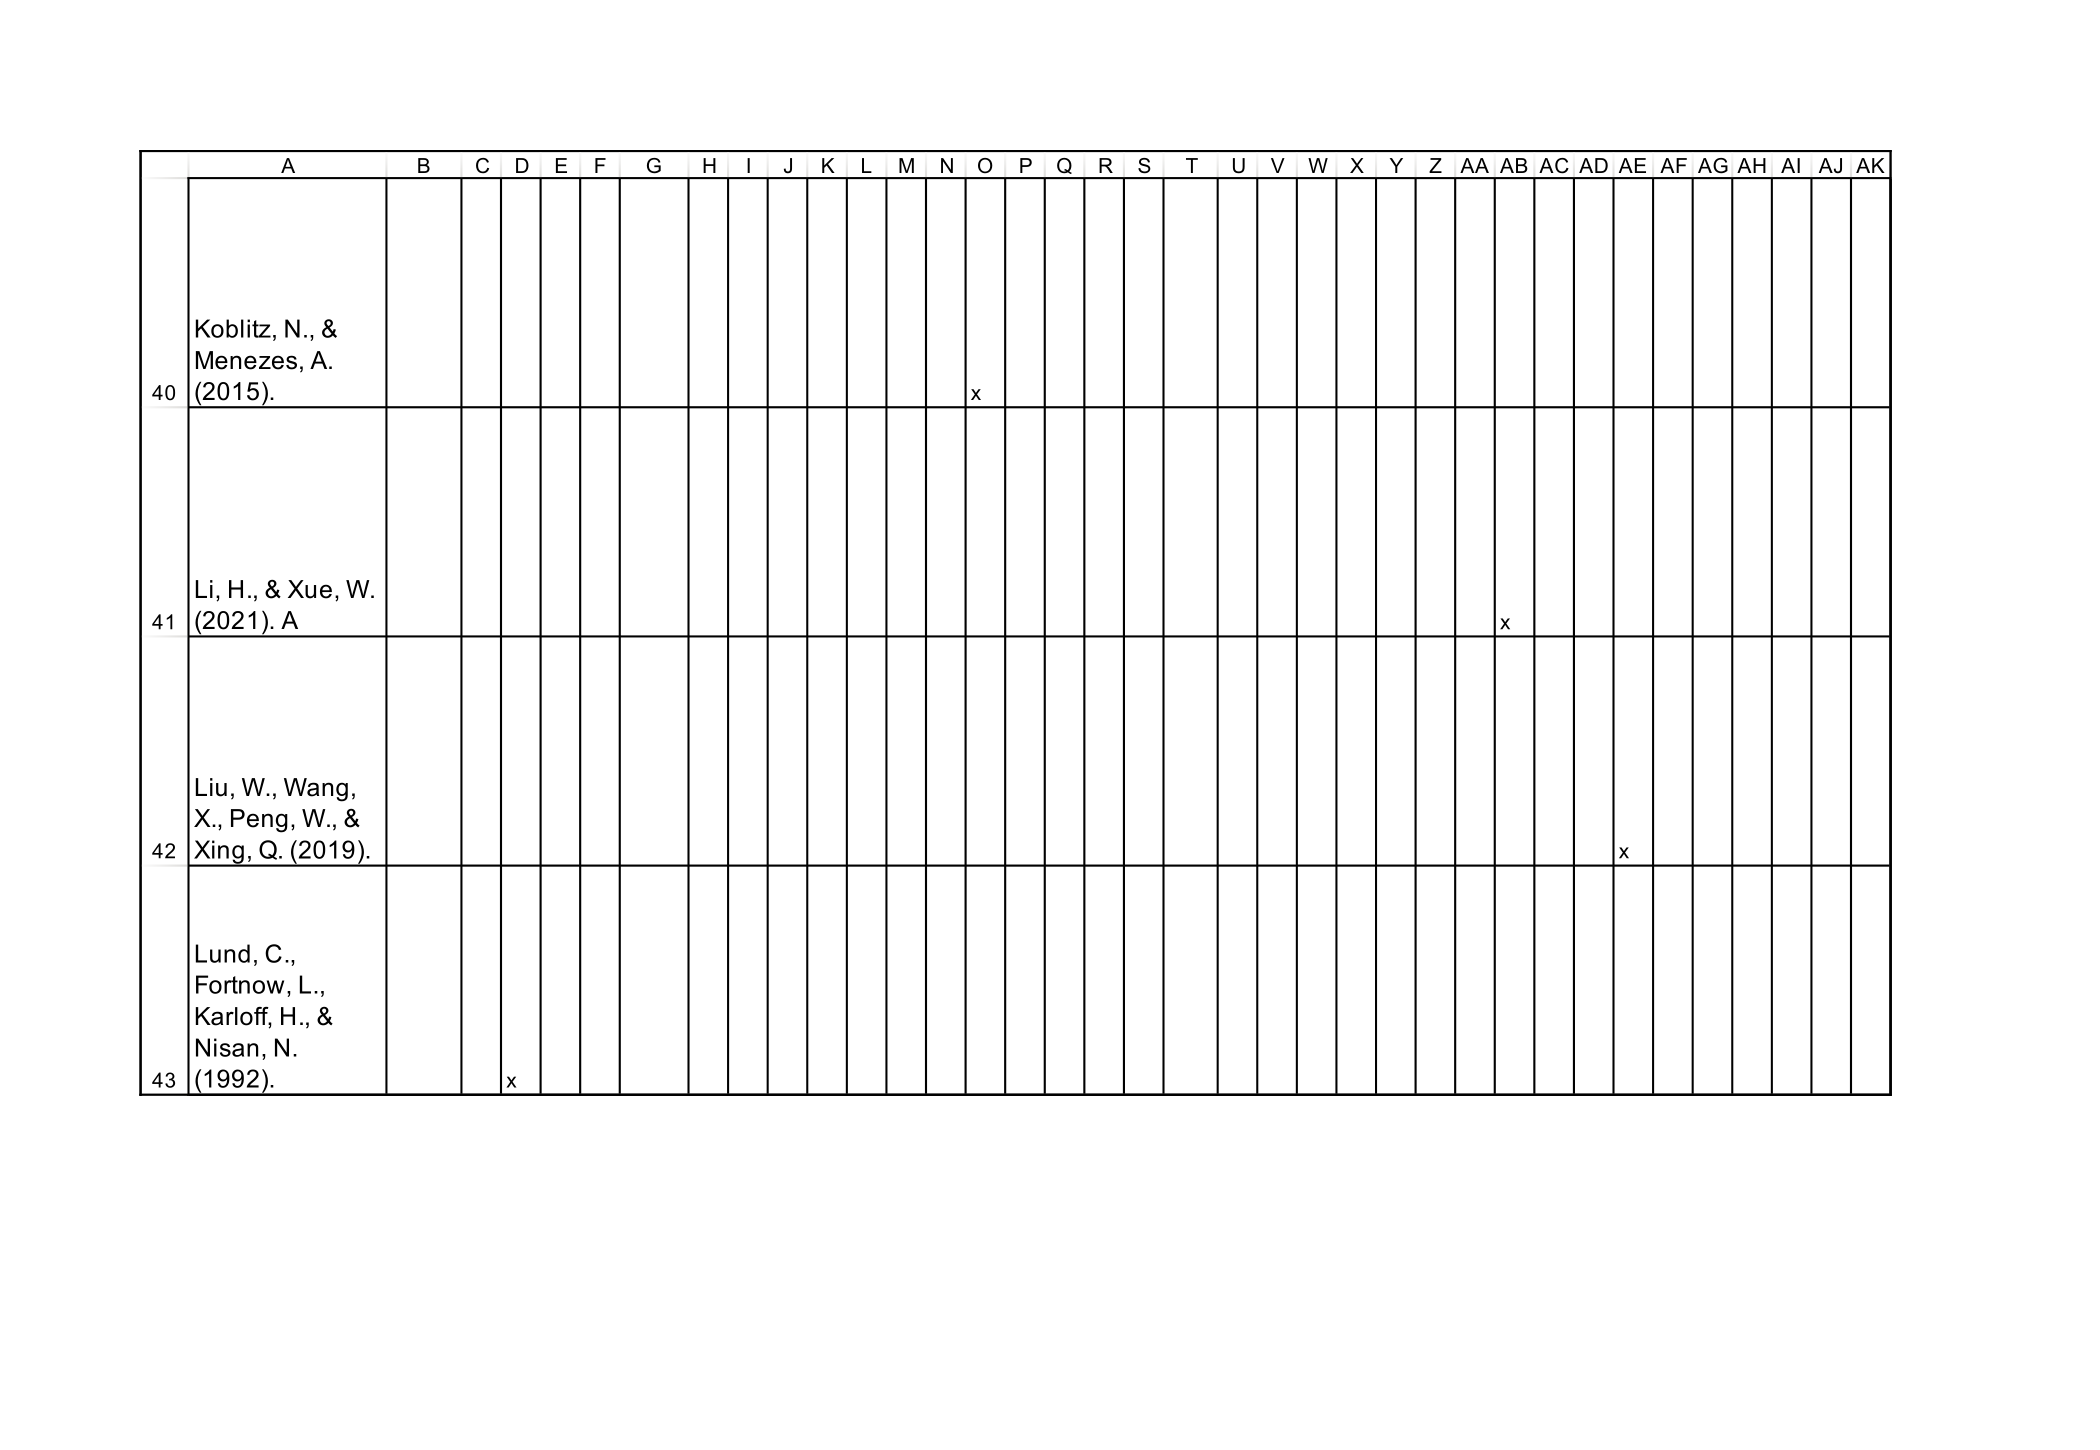
\includegraphics[width=.95\textwidth]{Pictures/concept_matrix/wos-11.png}
\end{figure}

\begin{figure}[H]
	\centering
		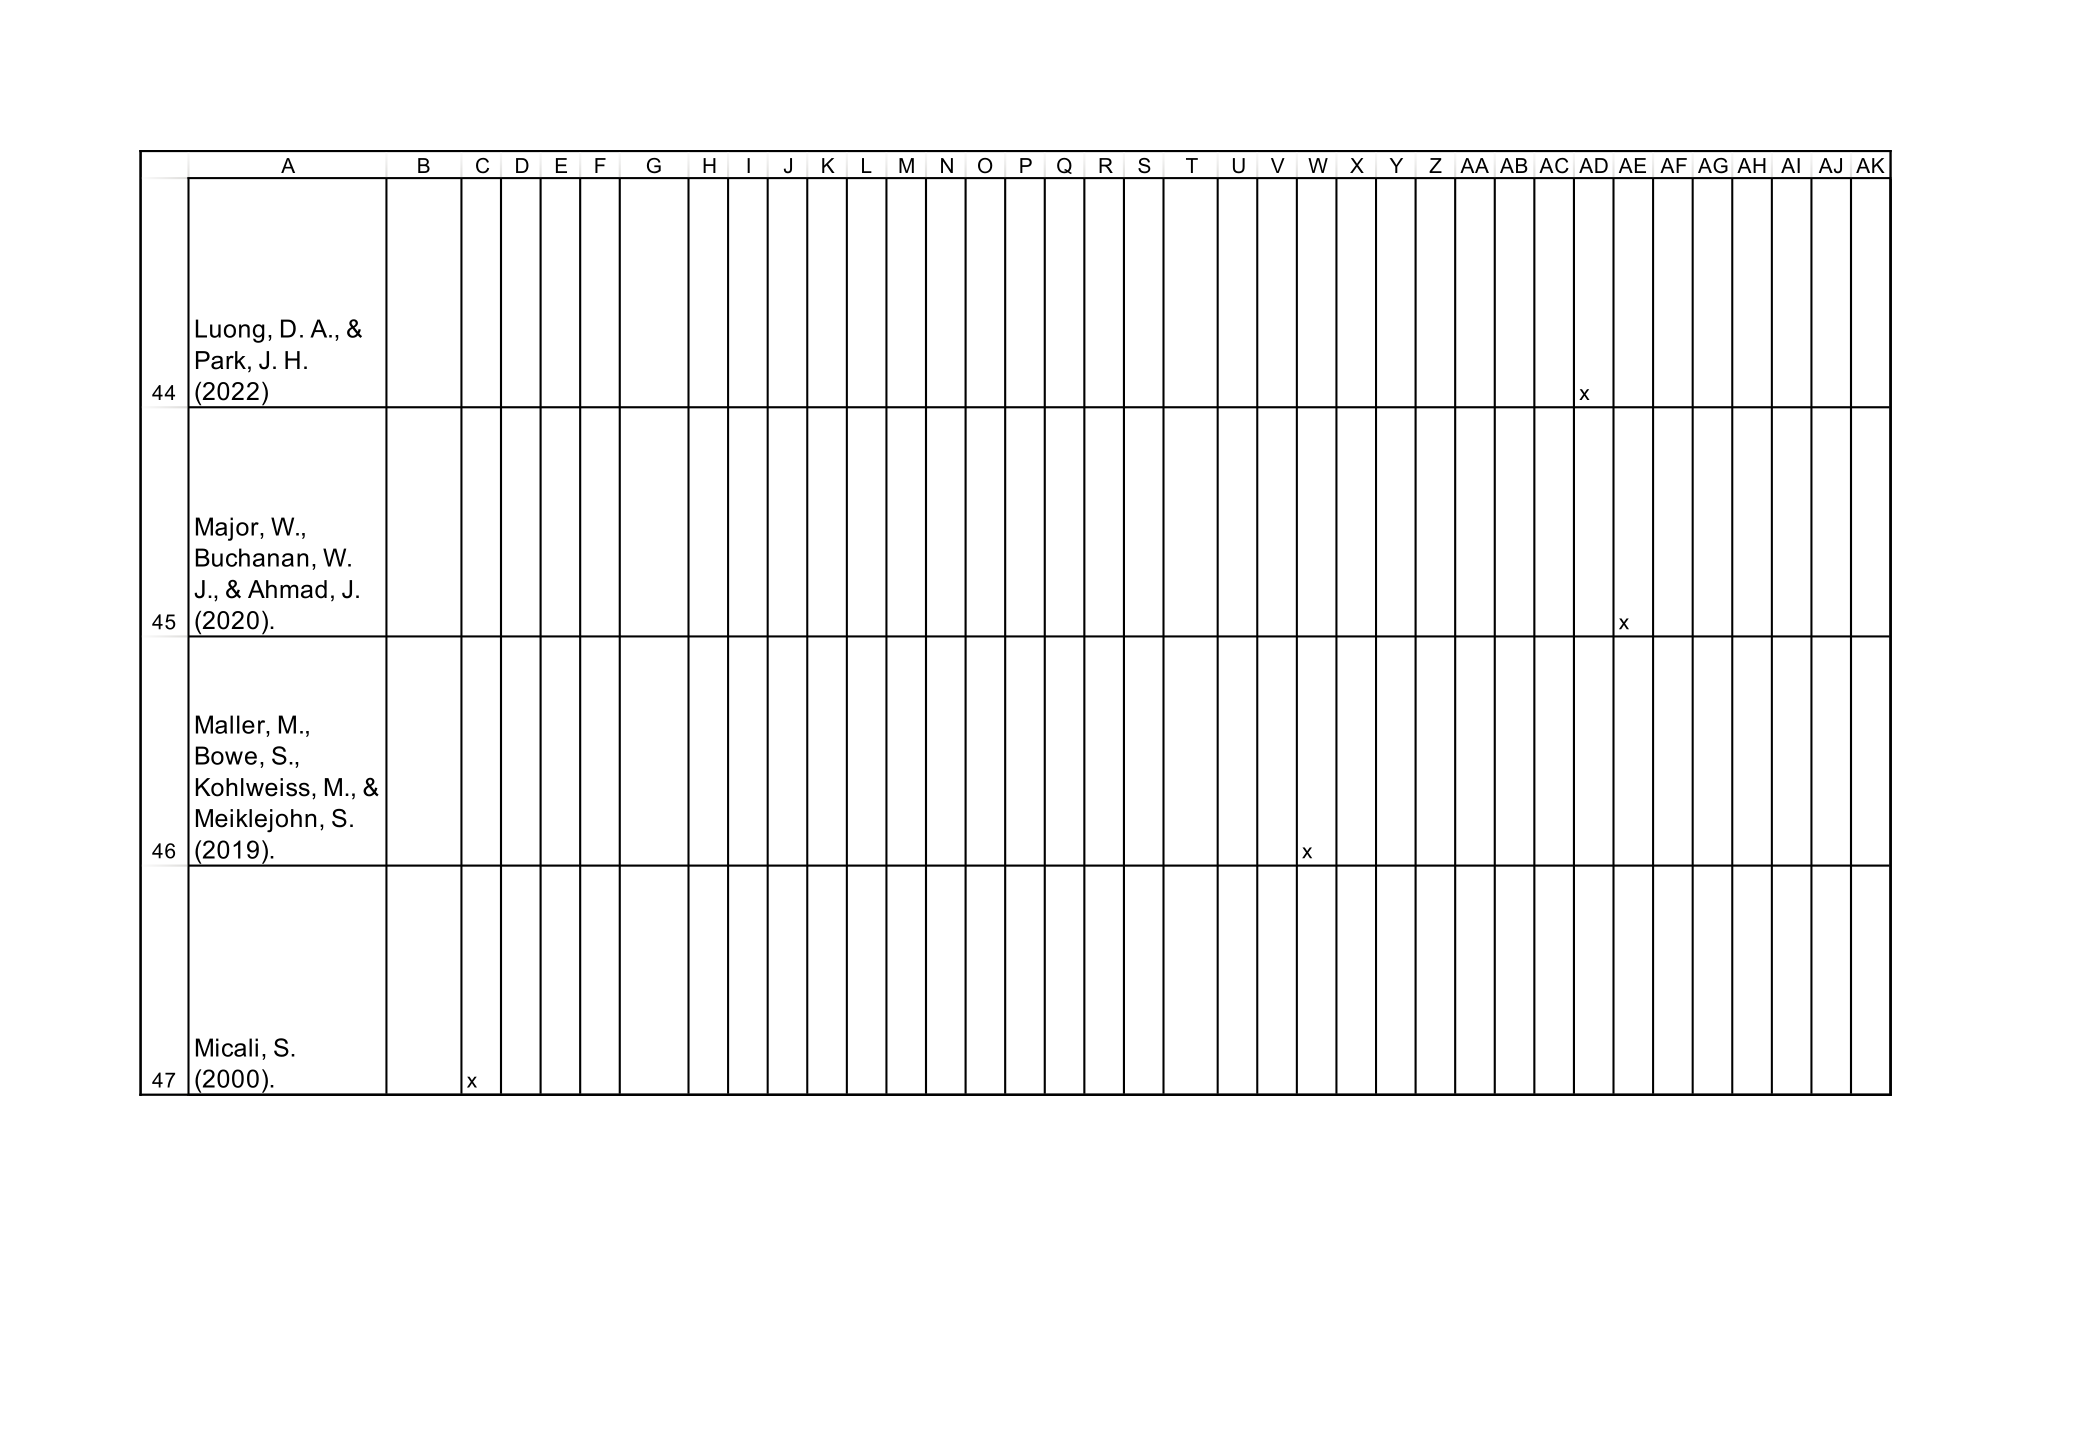
\includegraphics[width=.95\textwidth]{Pictures/concept_matrix/wos-12.png}
\end{figure}

\begin{figure}[H]
	\centering
		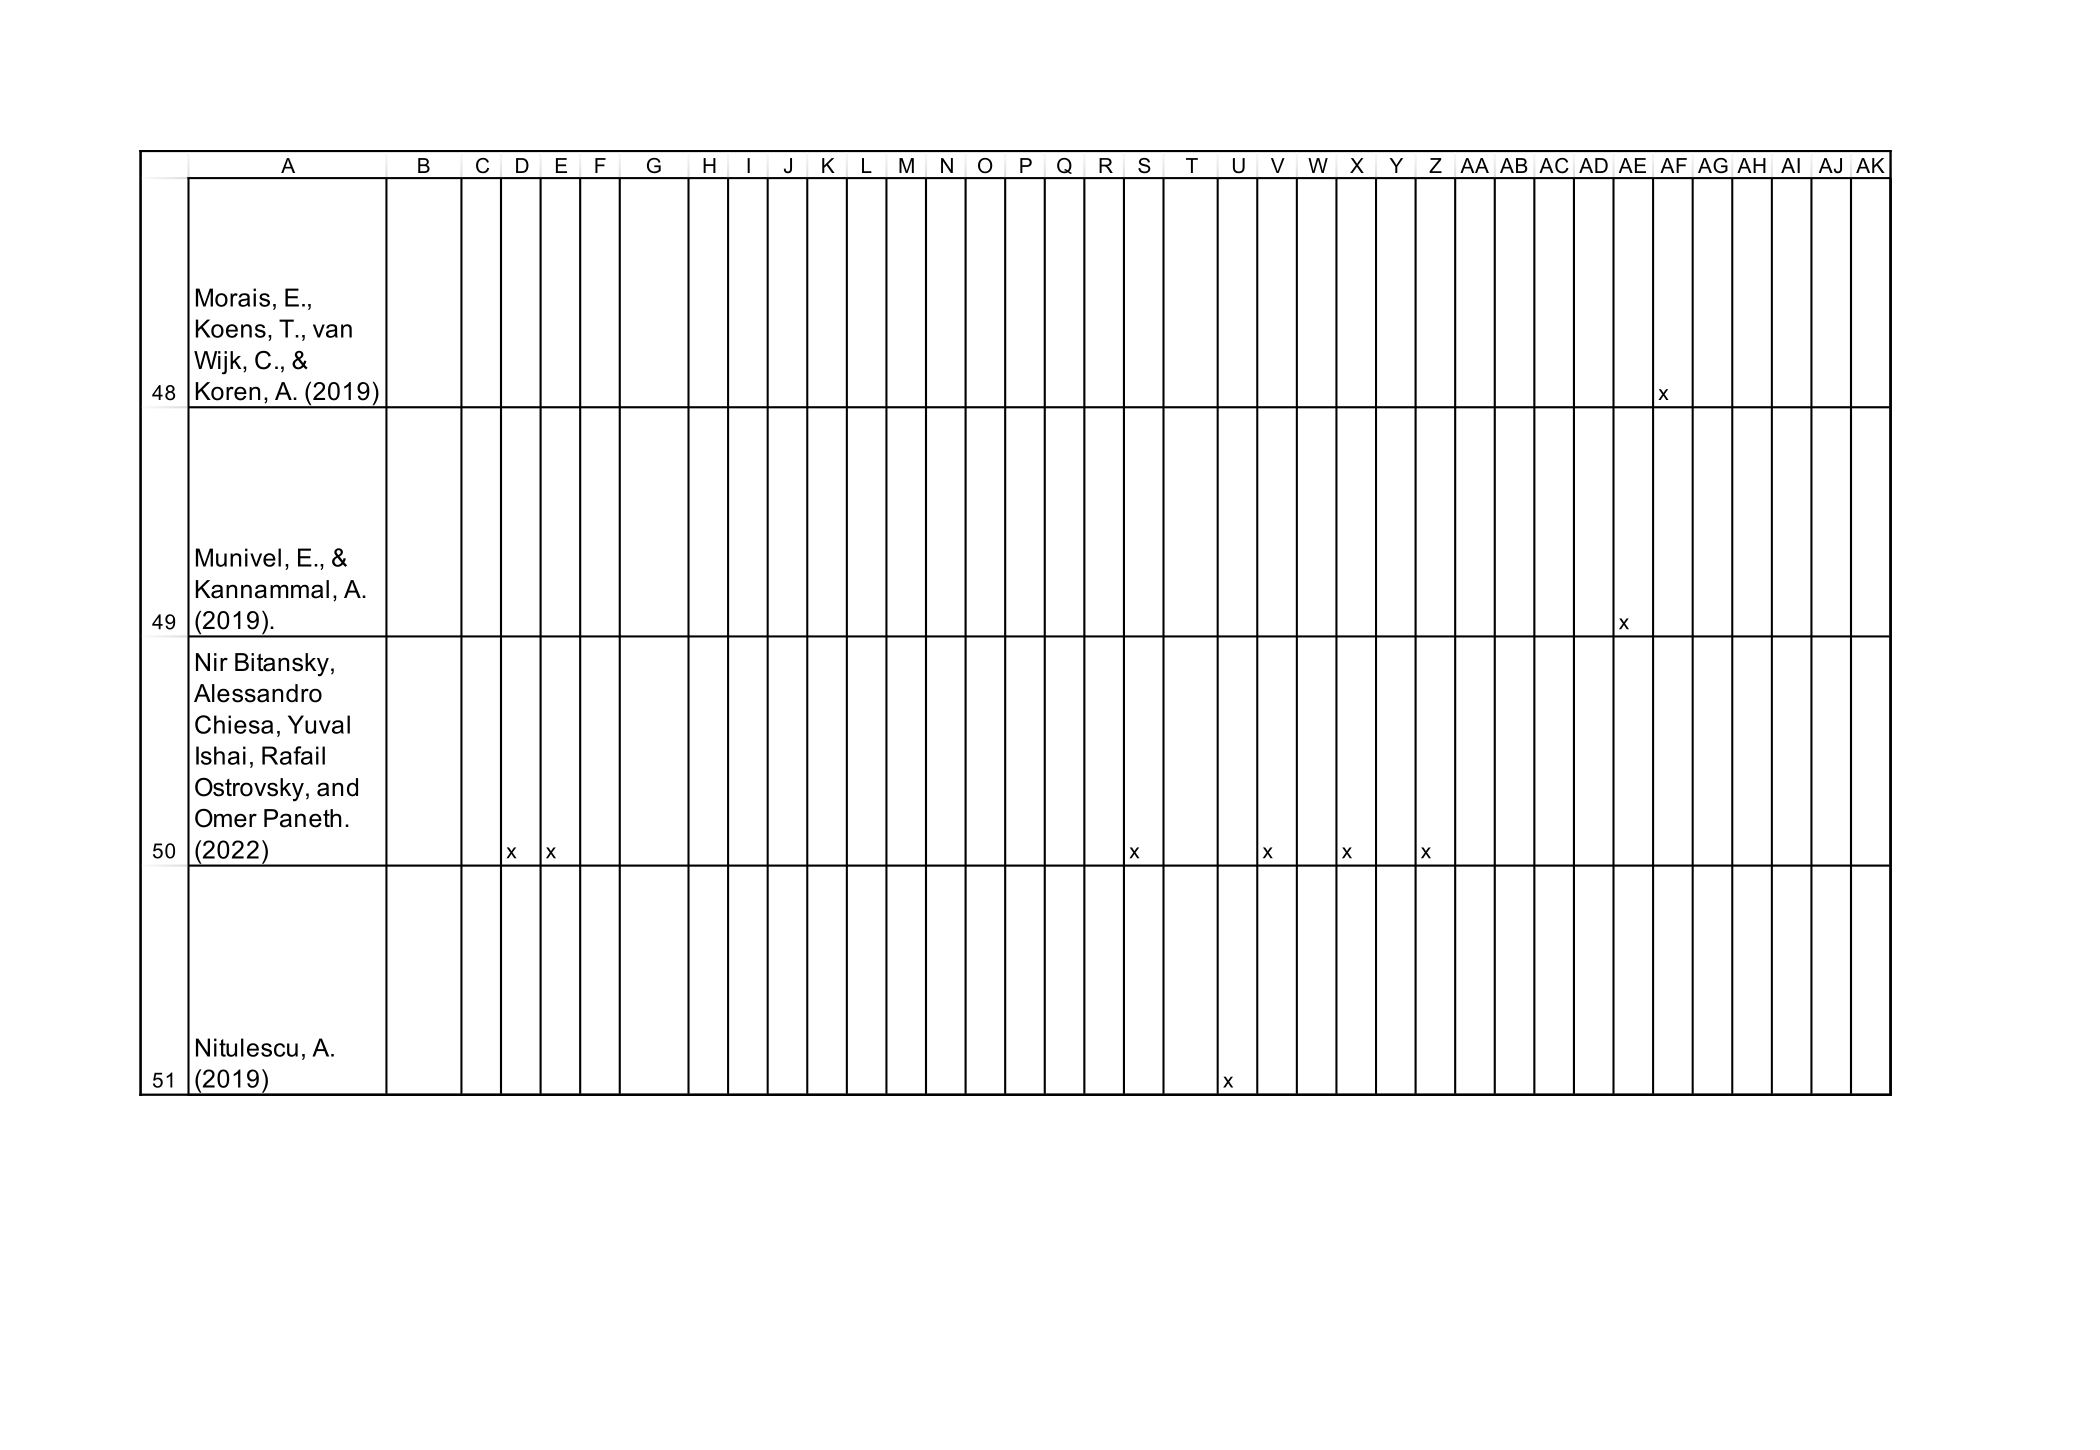
\includegraphics[width=.95\textwidth]{Pictures/concept_matrix/wos-13.png}
\end{figure}

\begin{figure}[H]
	\centering
		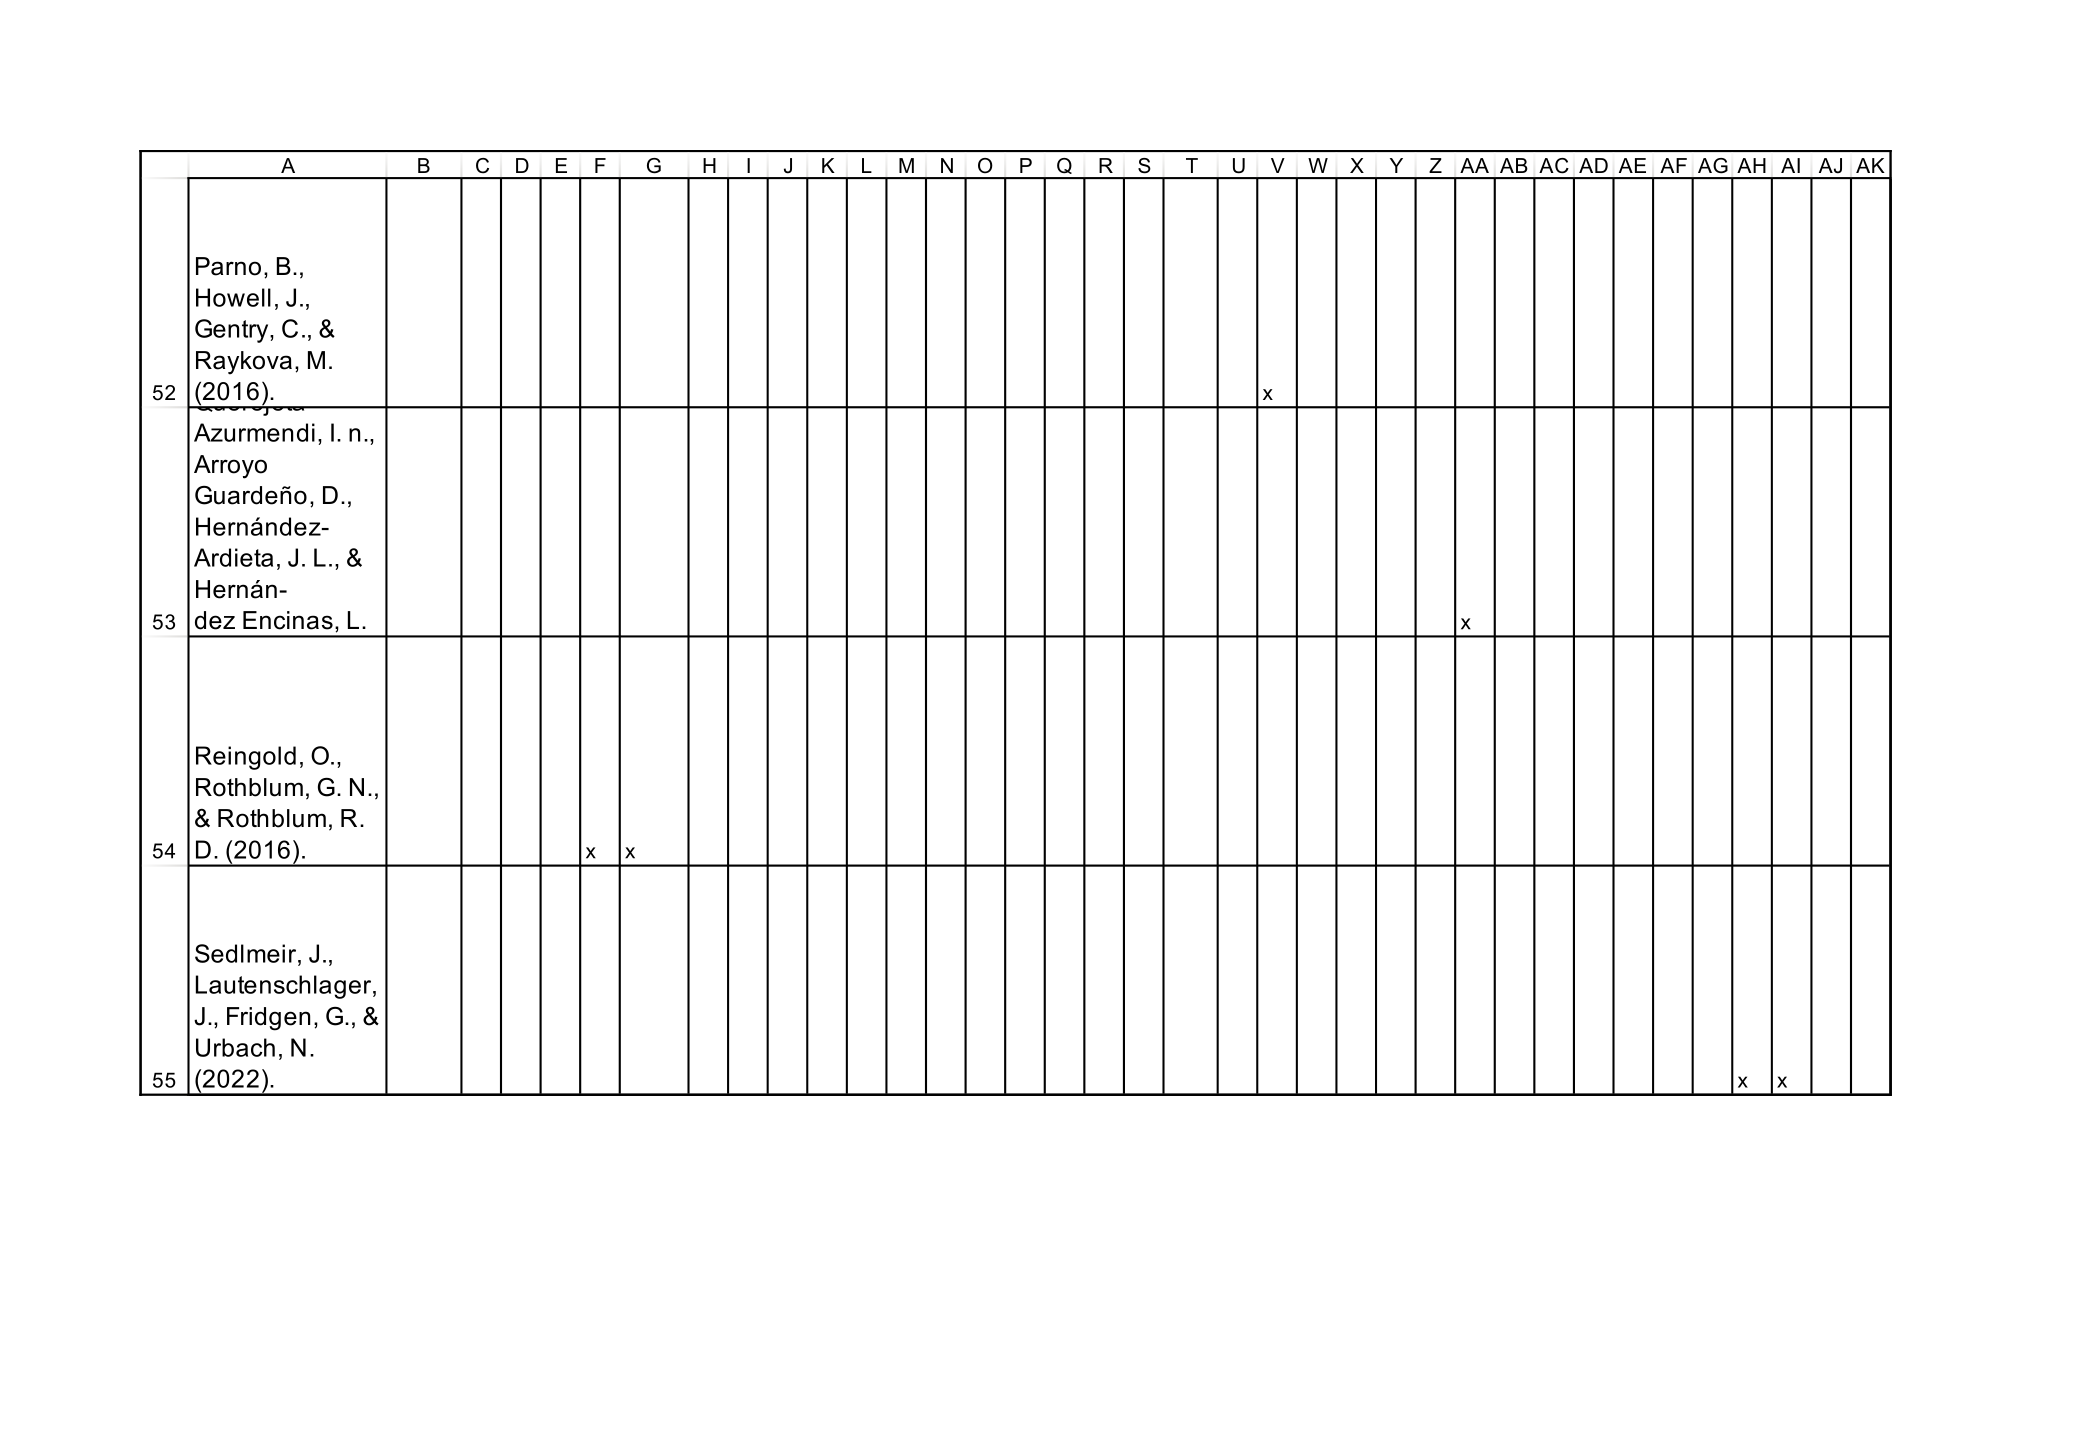
\includegraphics[width=.95\textwidth]{Pictures/concept_matrix/wos-14.png}
\end{figure}

\begin{figure}[H]
	\centering
		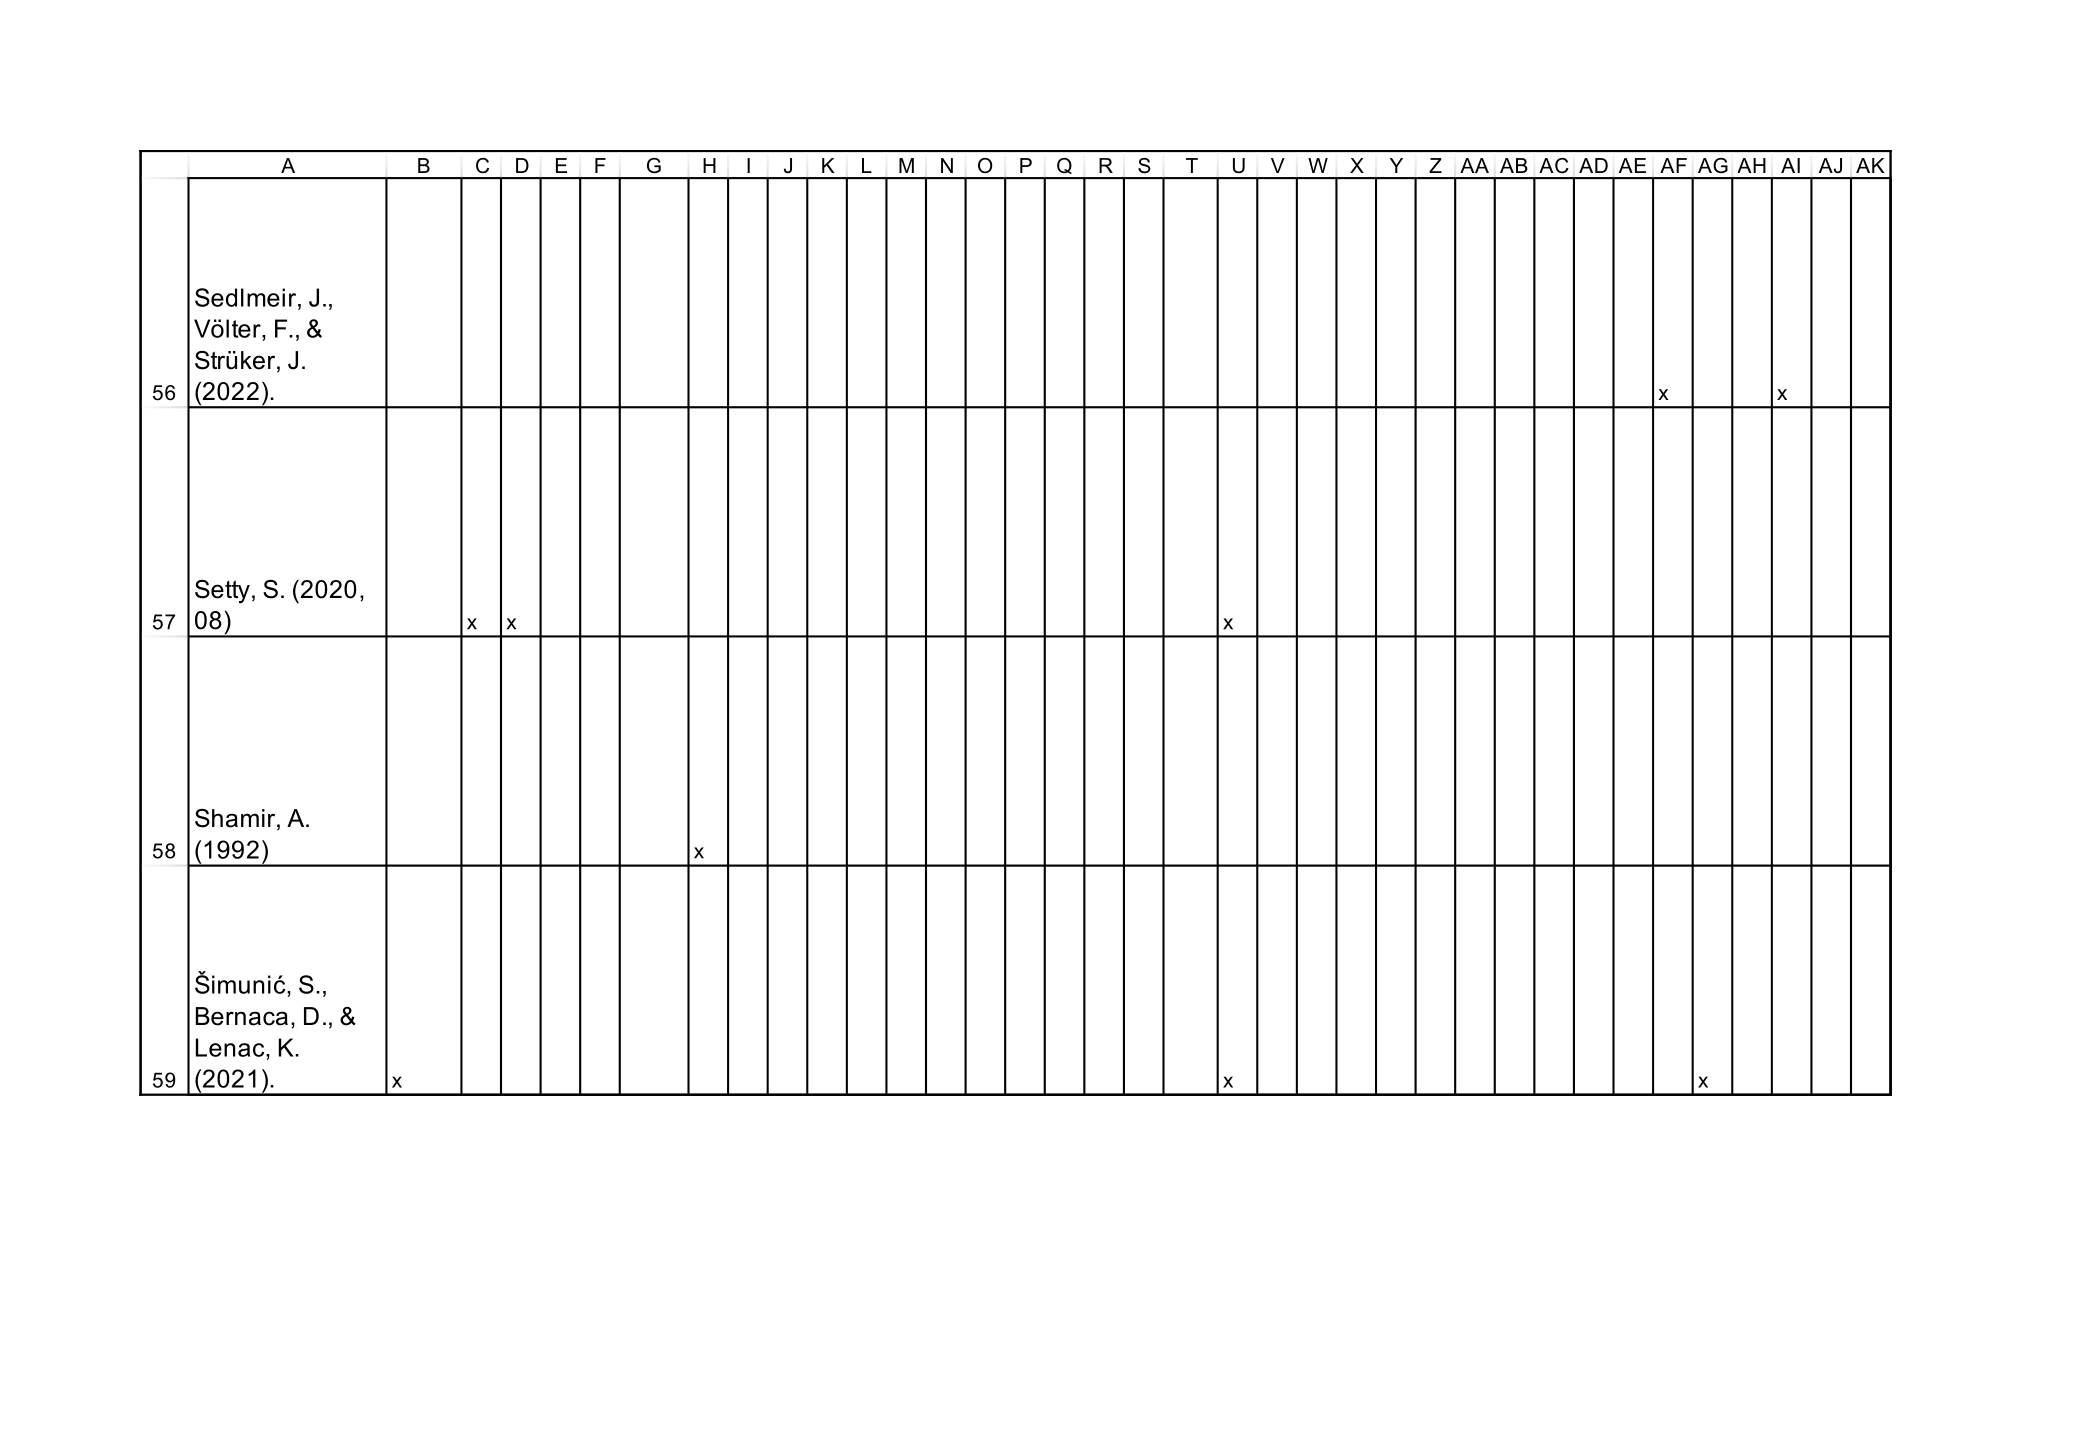
\includegraphics[width=.95\textwidth]{Pictures/concept_matrix/wos-15.png}
\end{figure}

\begin{figure}[H]
	\centering
		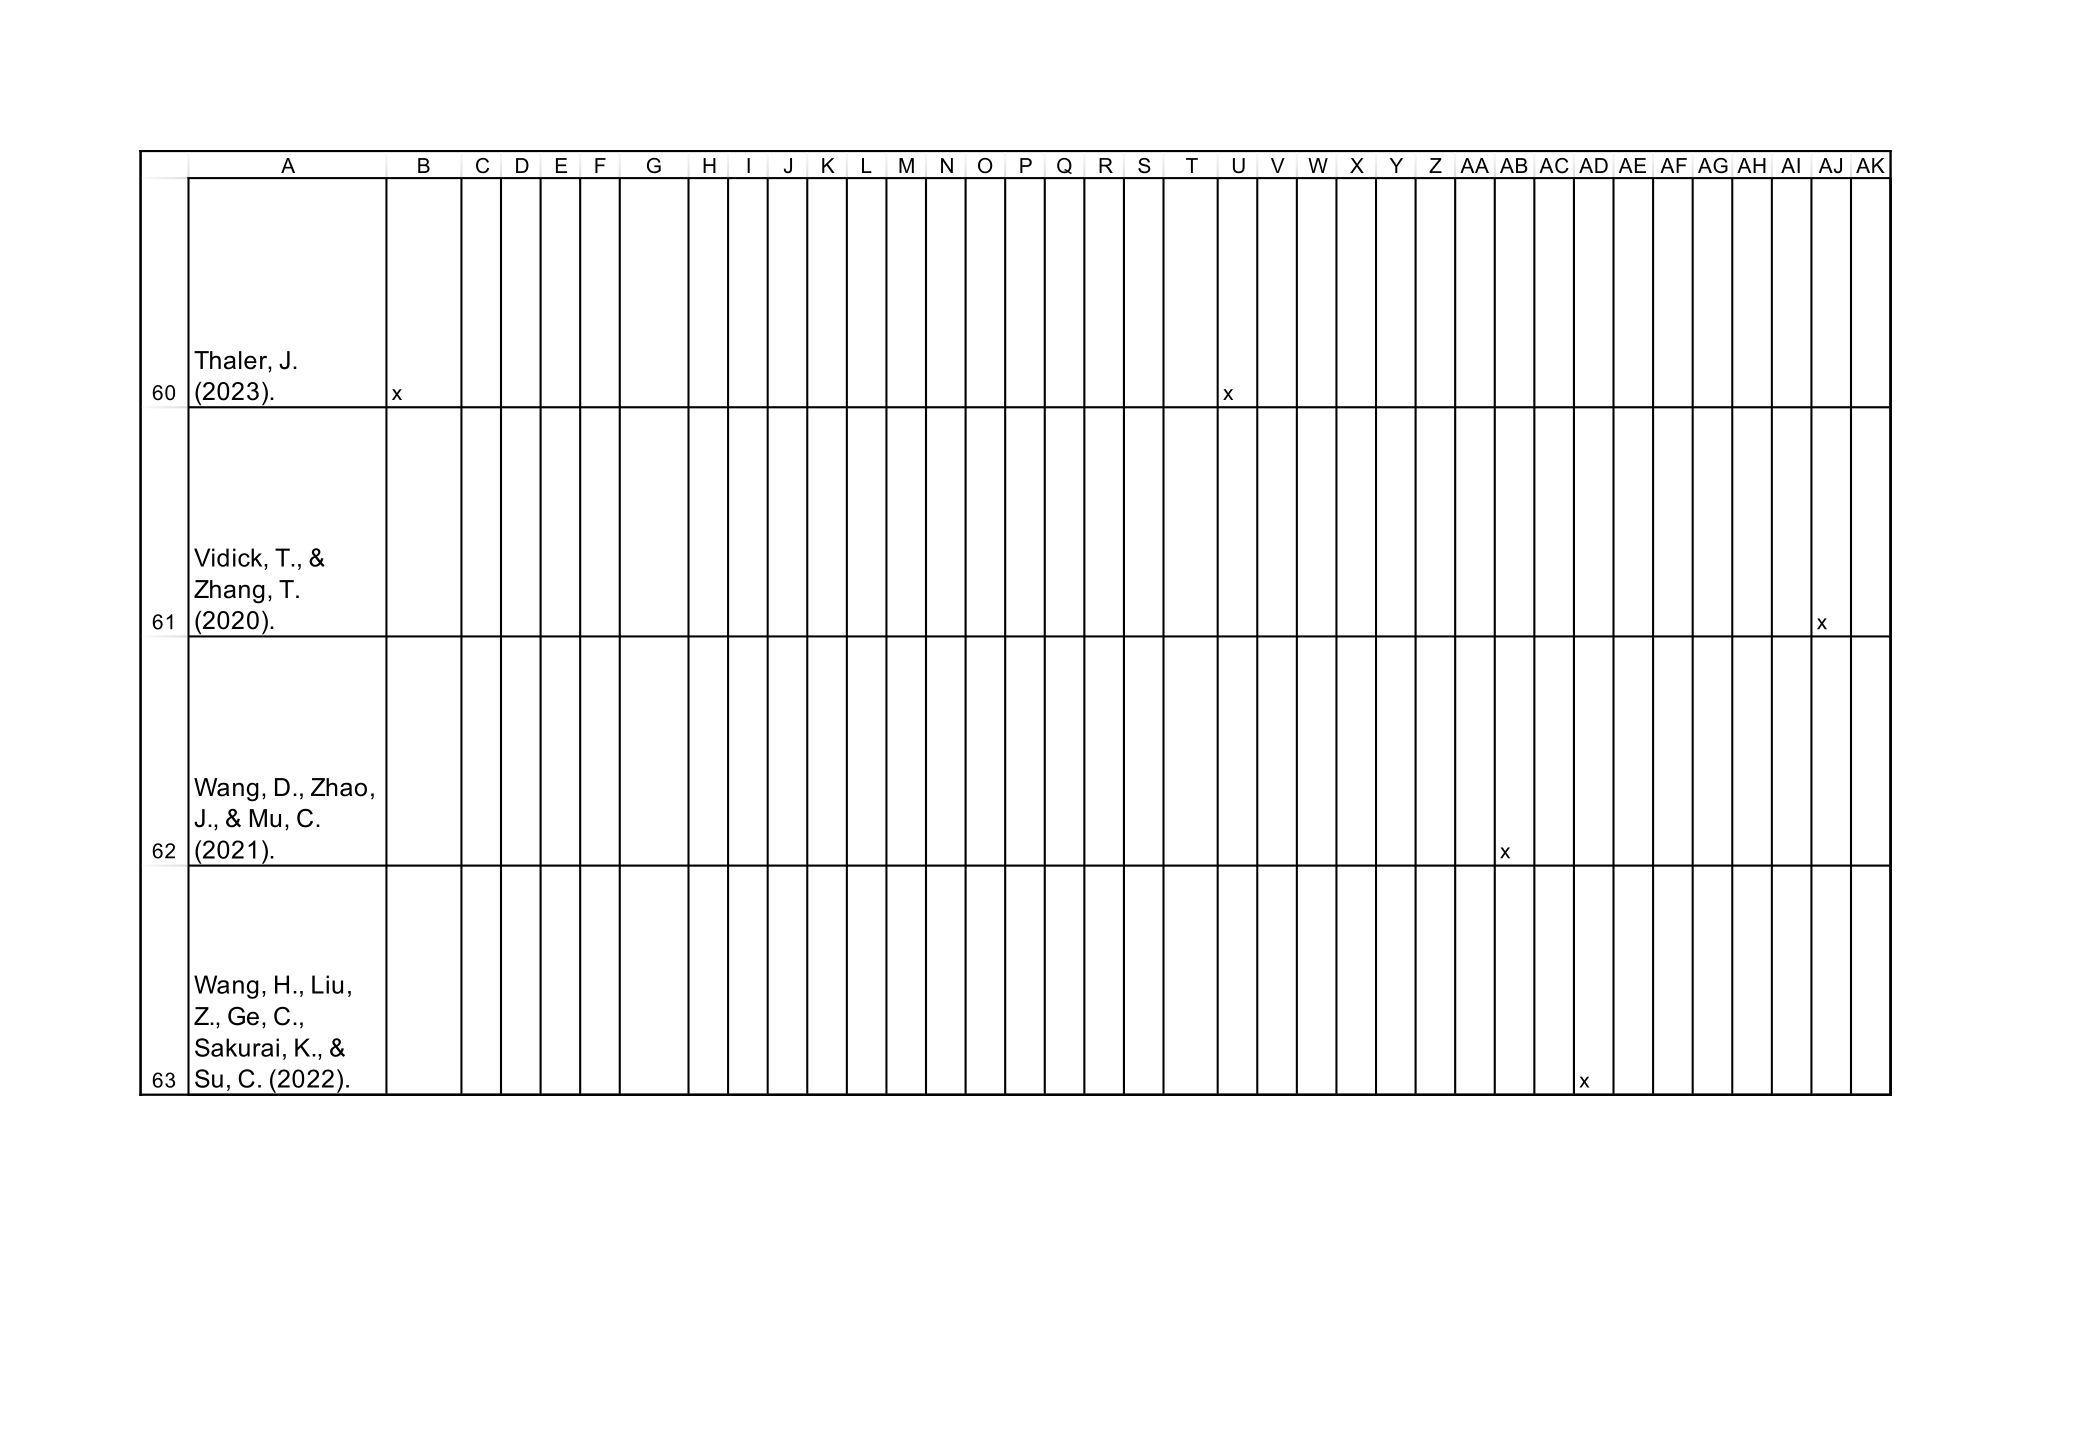
\includegraphics[width=.95\textwidth]{Pictures/concept_matrix/wos-16.png}
\end{figure}

\begin{figure}[H]
	\centering
		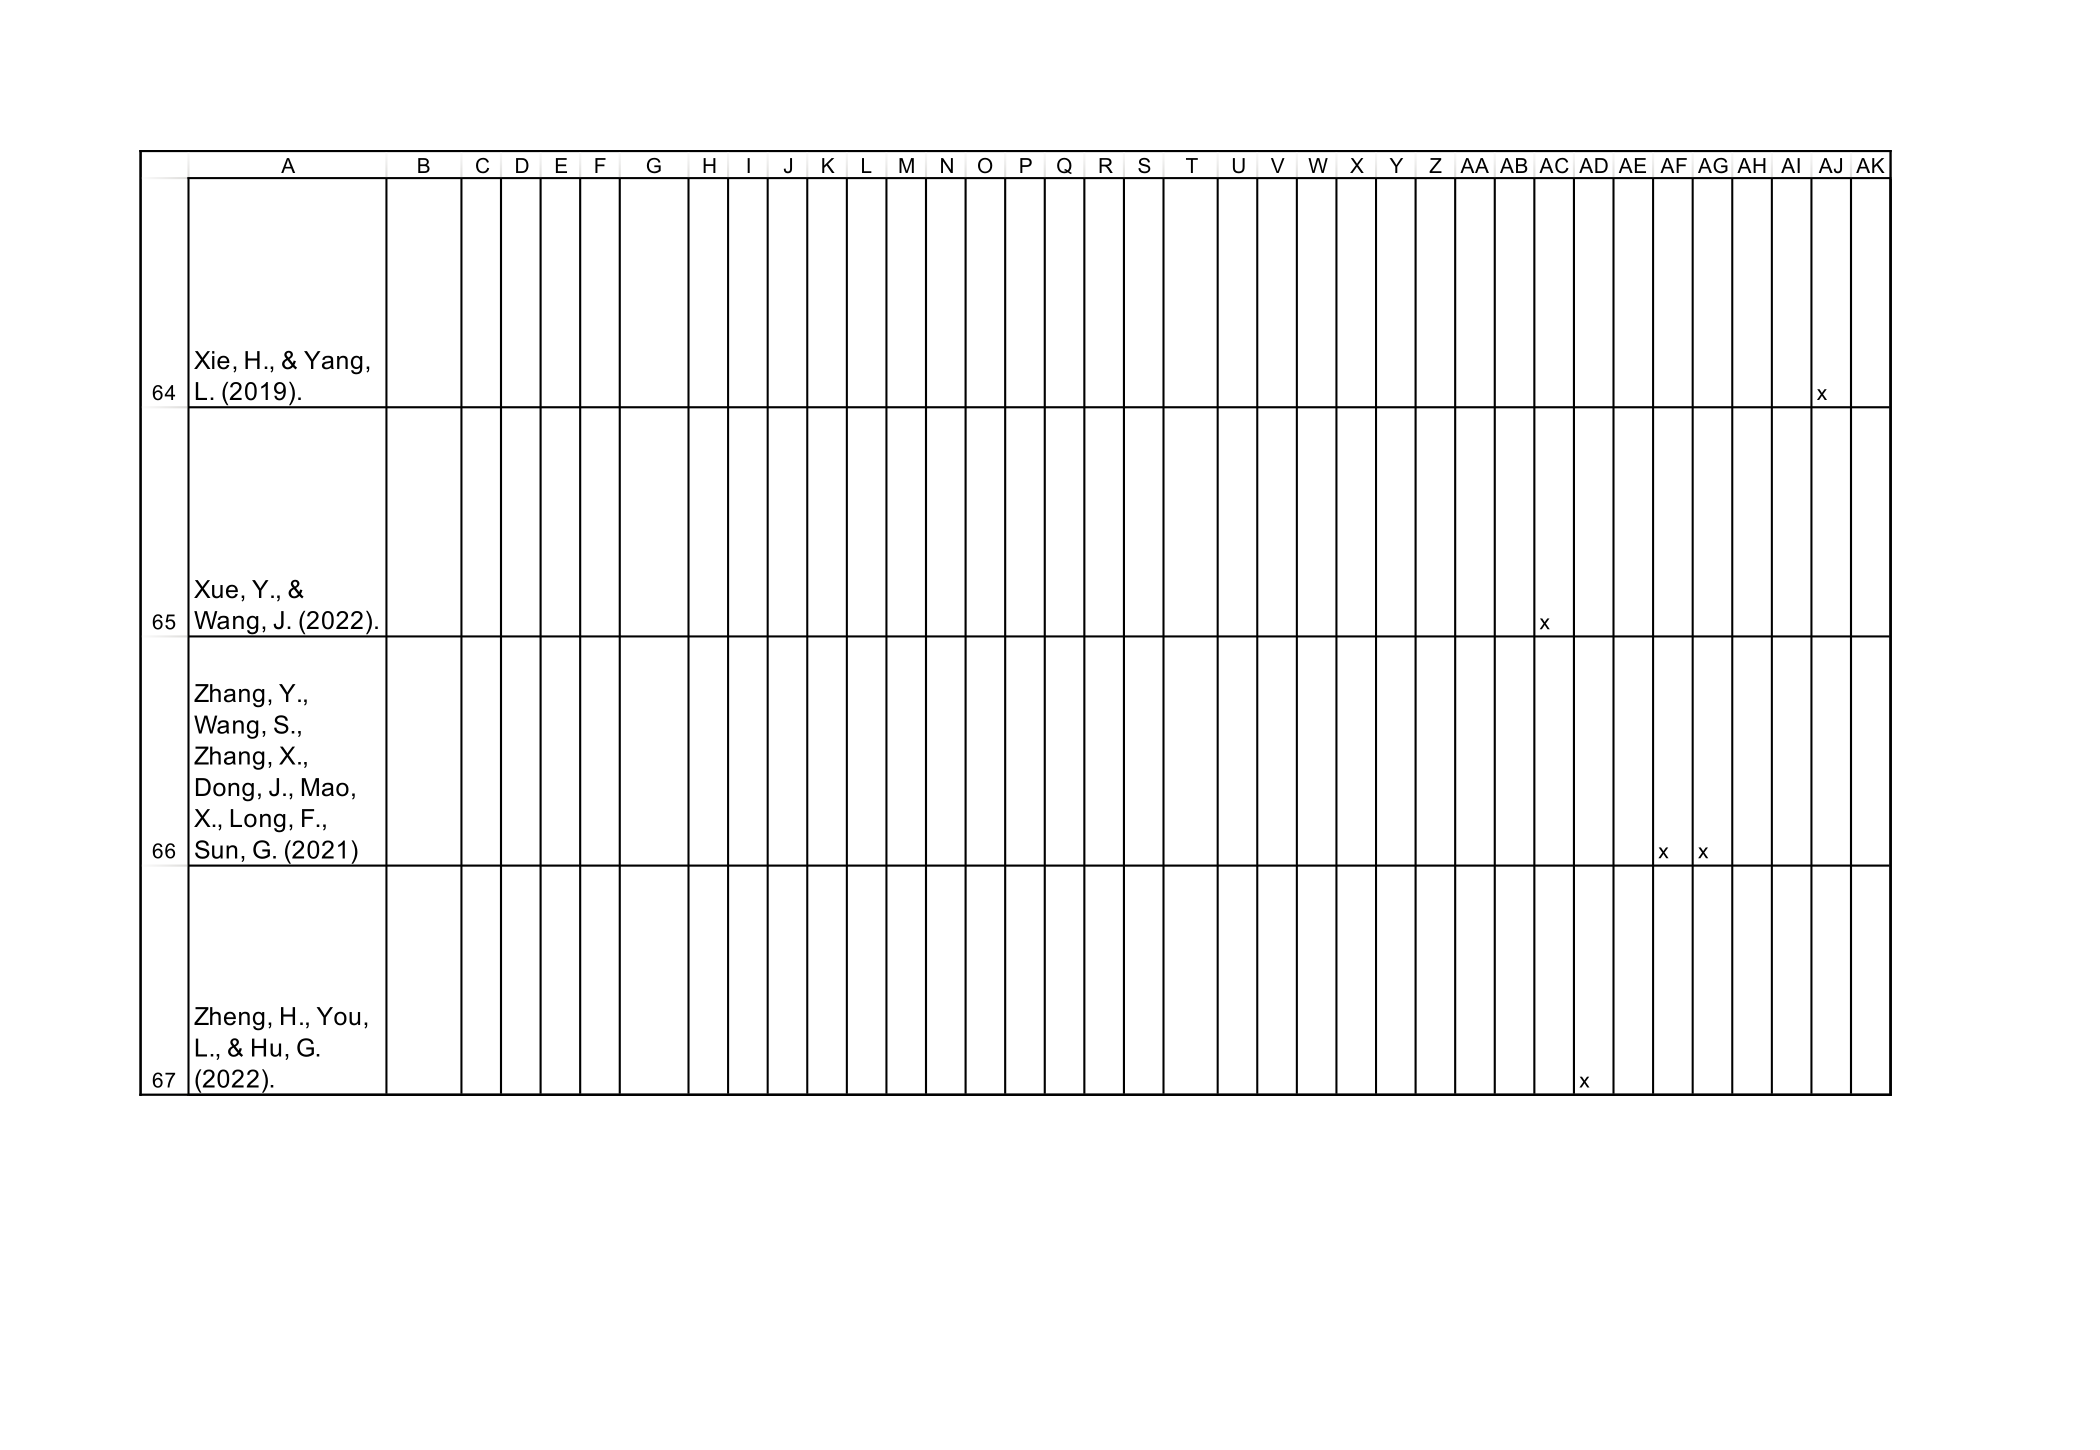
\includegraphics[width=.95\textwidth]{Pictures/concept_matrix/wos-17.png}
\end{figure}

\begin{figure}[H]
	\centering
		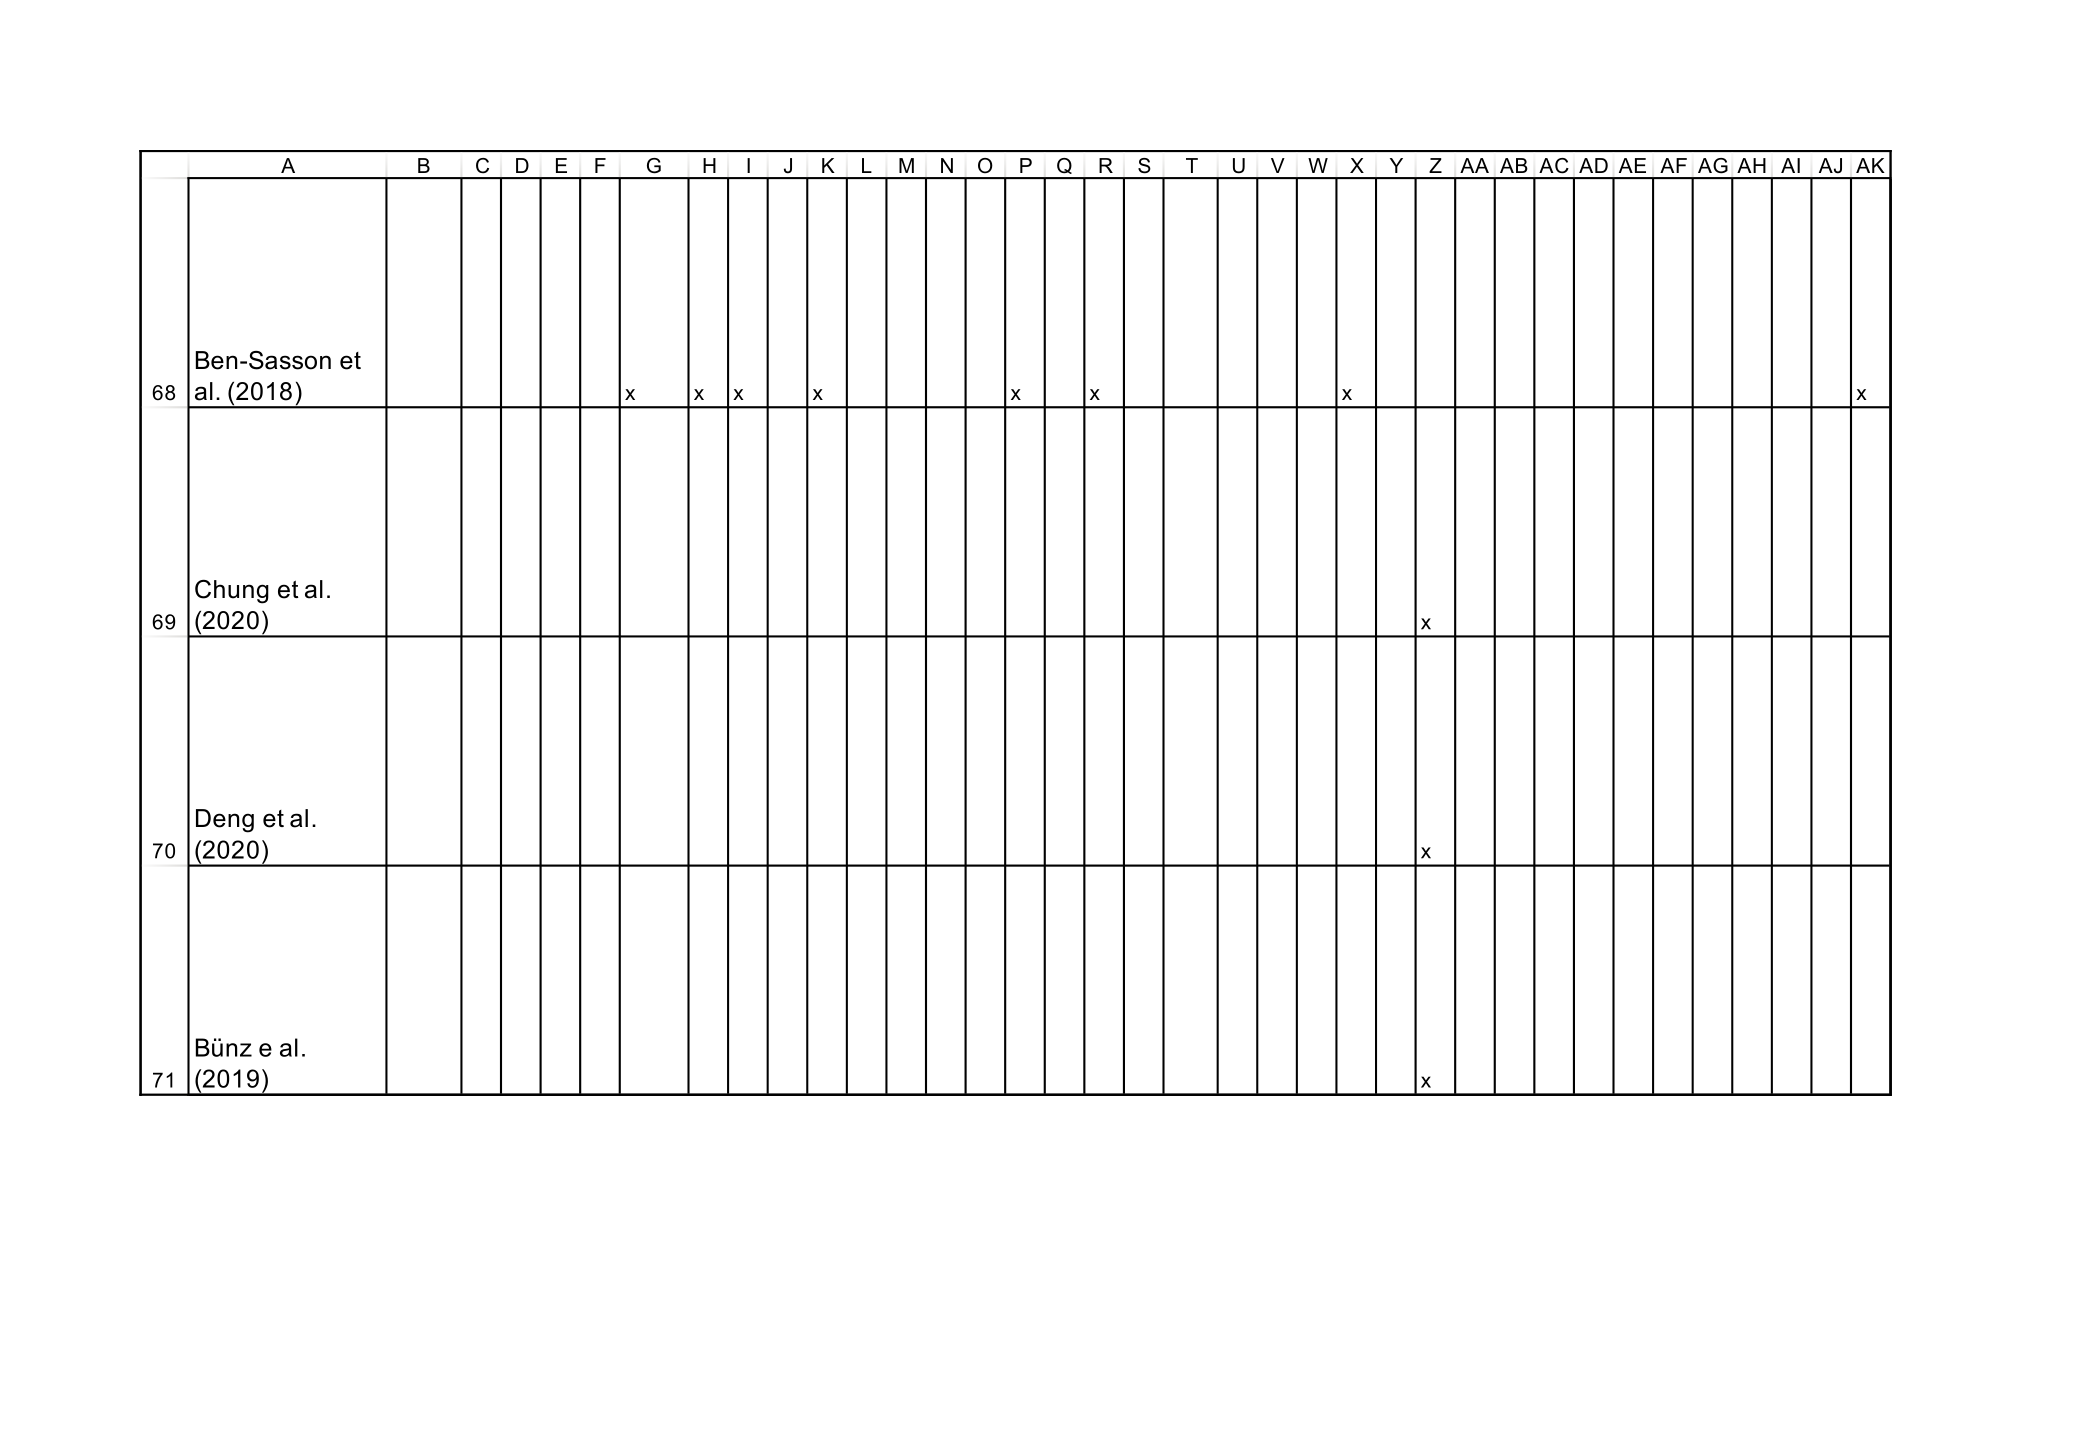
\includegraphics[width=.95\textwidth]{Pictures/concept_matrix/wos-18.png}
\end{figure}
\newpage
\subsection*{zk-DApp for MRO Attestations (Additional Screenshots)} \label{Appendix B}

\begin{figure}[H]
	\centering
		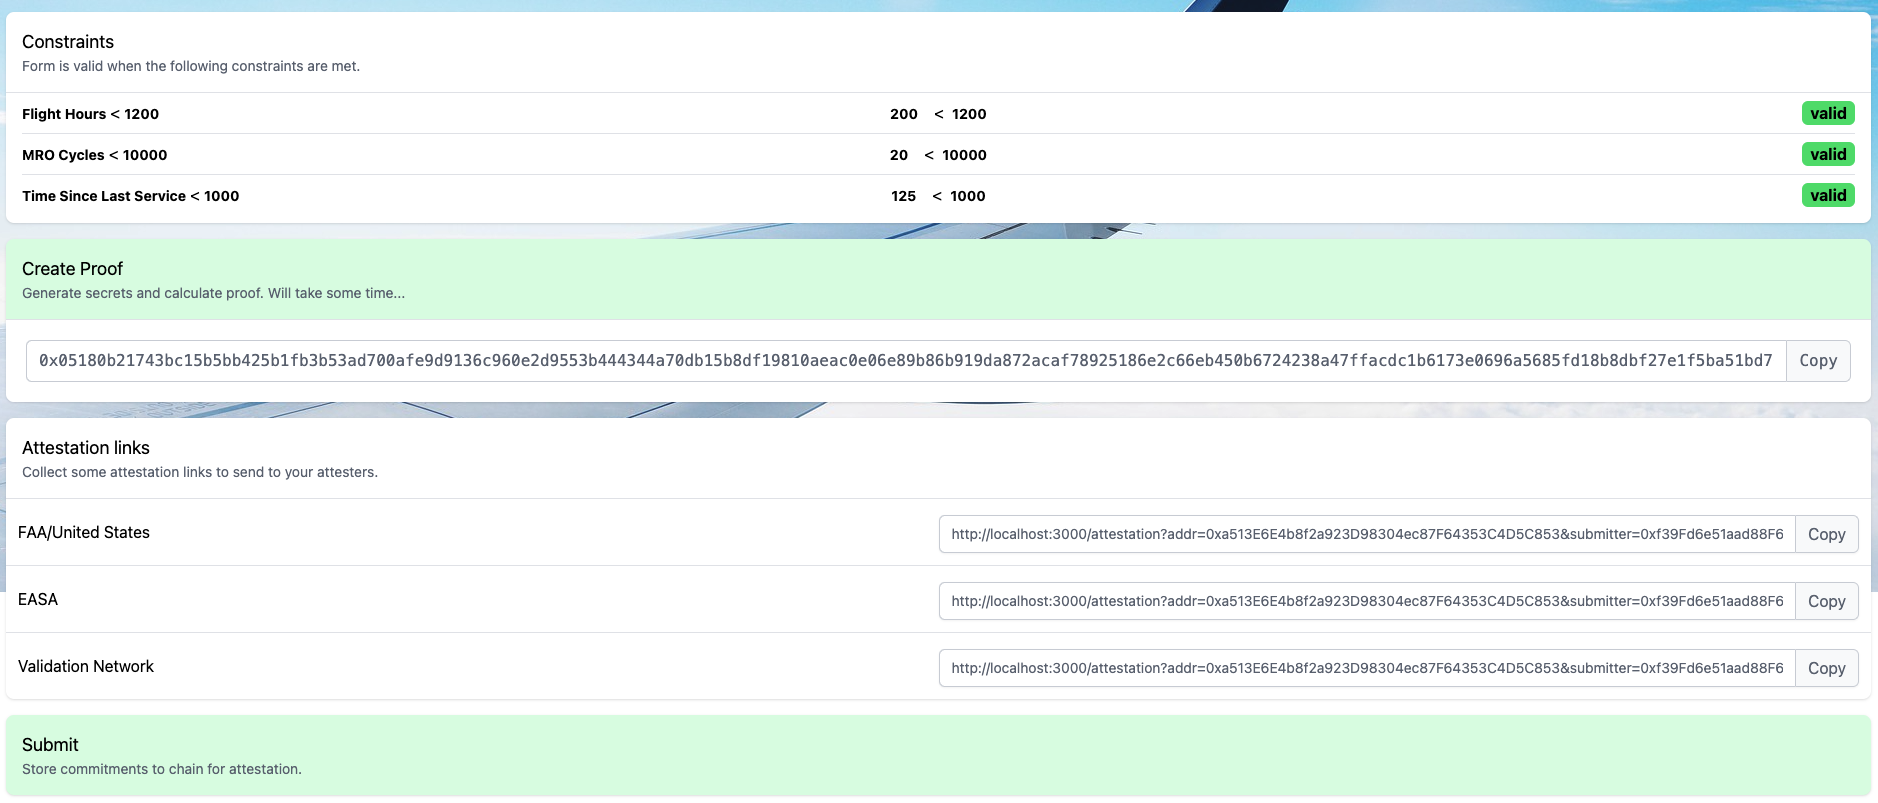
\includegraphics[width=1.0\textwidth]{Pictures/form_proof_const.png}
\end{figure}

\begin{figure}[H]
	\centering
		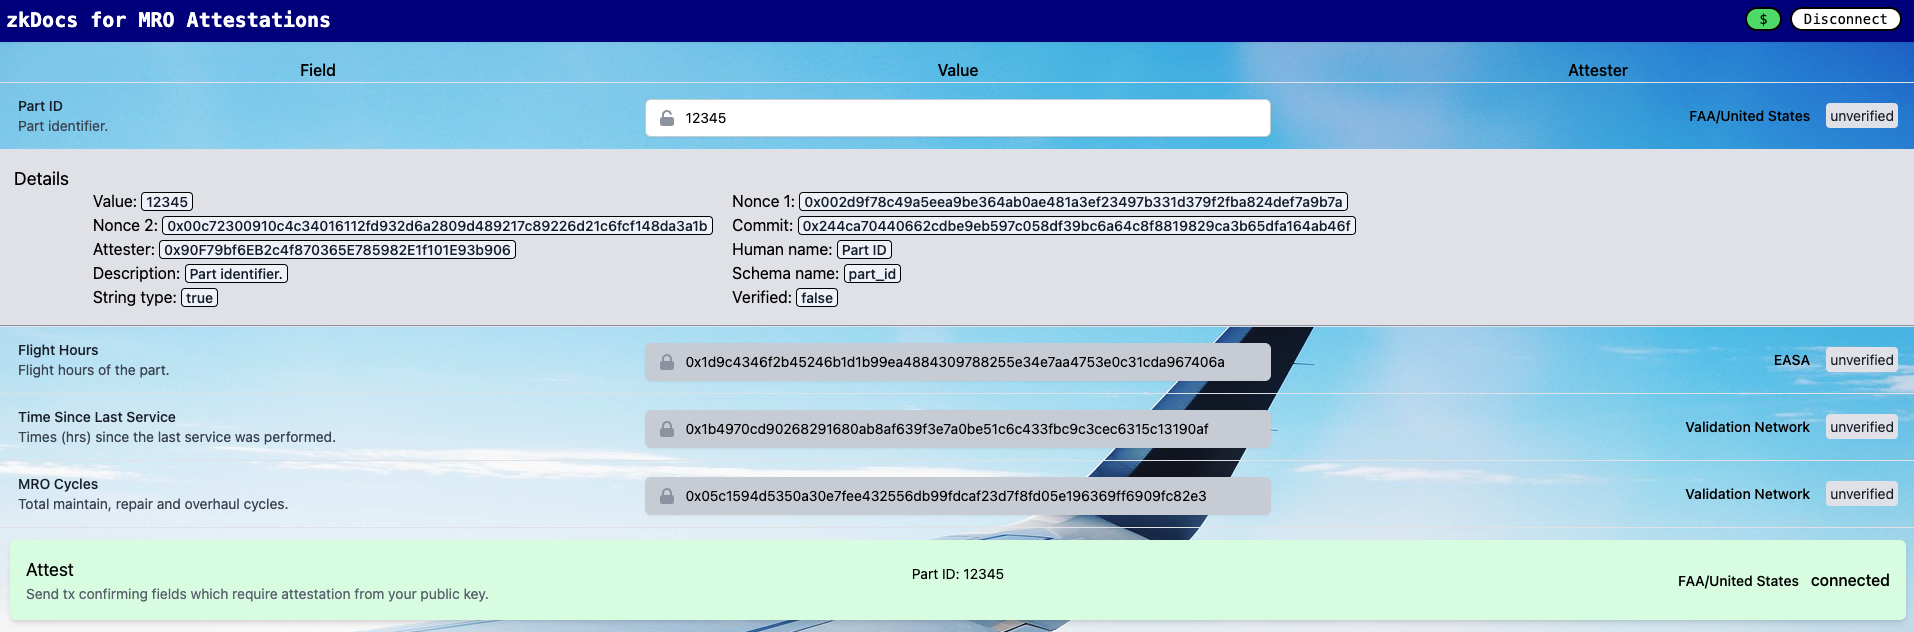
\includegraphics[width=1.0\textwidth]{Pictures/faa_attest_page.png}
\end{figure}           % Appendix
\clearpage{\pagestyle{empty}\cleardoublepage}
\newpage
\thispagestyle{empty}

\begin{large}

\vspace*{2cm}

\noindent
I declare that I have authored this thesis independently, that I have not used other than the declared
sources / resources, and that I have explicitly marked all material which has been quoted either
literally or by content from the used sources. 

\vspace{2cm}

\noindent
Berlin, 12 June 2023
\vspace{3cm}

\hspace*{\fill}
\begin{tabular}{l}  %% if you want centered alignment use 'c' instead of 'l'
Signature \\[1ex]
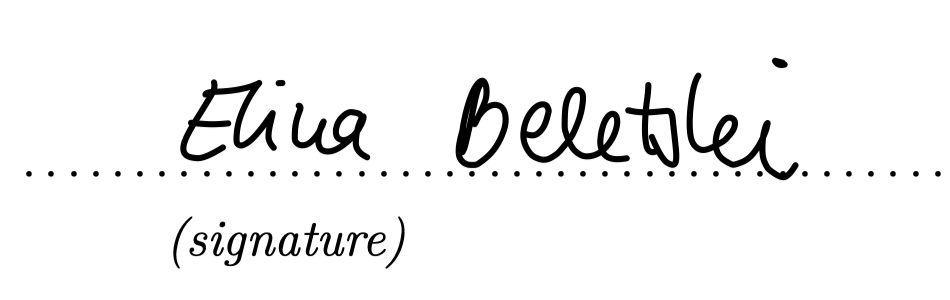
\includegraphics[scale=0.5]{Pictures/signature.png}
\end{tabular}
\end{large}
 % Eidesstattliche Erklärung (nicht bei Seminararb.)

\end{document}